\chapter{Oseen 方程}\label{chap:oseen}

\begin{note}[动机]\label{note:oseen-motivation}
Oseen 方程(Oseen equations)是一类线性方程,在许多求解 Navier--Stokes 方程的数值方法中充当辅助问题.\index{Oseen 方程}对 Navier--Stokes 方程作隐式时间离散后,每个离散时刻都需要求解一个非线性问题;稳态 Navier--Stokes 方程同样是非线性的.在这两种情形下,若用所谓的 Picard 方法(不动点迭代)求解非线性问题,每次迭代都会得到一个 Oseen 问题,见第\hyperref[sec:steady-ns-picard]{6.3 节}.对 Navier--Stokes 方程采用半隐式时间离散,则会在每个离散时刻直接得到 Oseen 问题,见笔记\hyperref[note:oseen-semi-implicit]{7.61}.因此,许多 Navier--Stokes 方程模拟方法都需要求解 Oseen 问题.此外,Oseen 方程理论中的一些结论也用于 Navier--Stokes 方程分析,例如定理\hyperref[thm:steady-ns-uniqueness]{6.20}中稳态 Navier--Stokes 方程弱解唯一性的证明.由此可见,研究 Oseen 问题的分析和数值分析具有基础性意义.

与 Stokes 方程相比,Oseen 方程多了对流项和反应项(reactive term);这两项都可能占主导.因此,除了 inf-sup 条件,还必须处理笔记\hyperref[note:dimensionless-difficulties]{2.19}提到的第三个困难.
\end{note}

\section{连续方程}\label{sec:oseen-continuous-equations}

\begin{note}[Oseen 方程]\label{note:oseen-equations}
Oseen 方程是线性稳态方程.与 Stokes 方程\hyperref[eq:stokes-strong]{(4.1)}相比,其动量方程包含对流项(convective term,即速度的一阶导数),还可能包含所谓的反应项(速度的零阶导数).Oseen 方程写作
\begin{equation}\label{eq:oseen-strong}
\begin{aligned}
  -\nu\Delta\bm{u}+(\bm{b}\cdot\nabla)\bm{u}
     +c\bm{u}+\nabla p&=\bm{f} &&\text{于 }\Omega,\\
  \nabla\cdot\bm{u}&=0 &&\text{于 }\Omega,
\end{aligned}
\end{equation}
其中 $\nu>0$,$\bm{b}$ 是给定的对流场,且须在某种意义下无散,详见笔记\hyperref[note:oseen-skew-symmetry]{5.6};对几乎所有 $\bm{x}\in\Omega$,有 $c(\bm{x})\ge c_0\ge0$;并且 $\bm{f}\in H^{-1}(\Omega)^d$.为应用第\hyperref[sec:abstract-saddle-point]{3.1 节}的抽象理论并开展有限元误差分析,本章为简化讨论,给 Oseen 方程配以齐次 Dirichlet 边界条件 $\bm{u}=\bm{0}$ 于 $\Gamma=\partial\Omega$.
\end{note}

\begin{note}[方程(5.1)中的系数]\label{note:oseen-coefficients}
\begin{itemize}
  \item 若按物理量纲理解式\hyperref[eq:oseen-strong]{(5.1)}中的函数,则动量方程各项的单位都是 $\mathrm{m}/\mathrm{s}^2$.因此,函数 $c$ 的单位必须是 $1/\mathrm{s}$;也就是说,若 $c(t,\bm{x})>0$,则 $c^{-1}(t,\bm{x})$ 表示一个时间尺度.下文还会讨论这一点.
  \item 令 $\bm{b}\in L^\infty(\Omega)^d$.本章始终假设动量方程已作缩放,使下列两种情形之一成立:
  \begin{itemize}
    \item $\|\bm{b}\|_{L^\infty(\Omega)}\sim1$,若 $\nu\le\|\bm{b}\|_{L^\infty(\Omega)}$;
    \item $\nu\sim1$,若 $\|\bm{b}\|_{L^\infty(\Omega)}\le\nu$.
  \end{itemize}
  第一种情形更有实际意义.
  \item 式\hyperref[eq:oseen-strong]{(5.1)}中的其他系数有以下几种值得关注的情形:
  \begin{itemize}
    \item $\nu$ 取中等大小,且 $c=0$.若通过固定点迭代求解稳态 Navier--Stokes 方程,这一情形就会出现,见笔记\hyperref[note:steady-ns-picard-iteration]{6.41}.从应用角度看,稳态 Navier--Stokes 方程的极限 $\nu\to0$ 并不重要,因为当 $\nu$ 很小、Reynolds 数很大时,预期会出现含时解.严格来说,对稳态 Navier--Stokes 方程作有限元离散时,本章对 Oseen 问题系数所作的假设通常并不满足,参见笔记\hyperref[note:steady-ns-picard-iteration]{6.41}.
    \item $\nu$ 可取任意大小,且 $c=\mathcal{O}((\Delta t)^{-1})$.当 $\nu$ 较小时,预期会出现含时解;当 $\nu$ 极小时,甚至会出现湍流解.在含时问题中,$c\bm{u}$ 这一项来自隐式或半隐式时间离散,此时 $c=\mathcal{O}((\Delta t)^{-1})$,其中 $\Delta t$ 是时间步长,参见式\hyperref[eq:general-theta-picard]{(7.85)}.因此,时间步长较小时,$c\bm{u}$ 可能成为式(5.1)中的主导项.总的来说,对较宽范围的 $\nu$ 和 $c$,这一情形都有意义.
  \end{itemize}
  \item 在出现 Oseen 问题的数值方法中,$\bm{b}$ 是计算得到的速度场,通常就是当前已有的有限元解.一般而言,$V_{\mathrm{div}}^h\not\subset V_{\mathrm{div}}$,所以这一速度场通常并非弱无散.若采用满足 inf-sup 条件的有限元空间对,且代数鞍点问题得到精确求解,则该速度场是离散无散的.不过,实际计算往往也不会精确求解代数问题,因此 $\bm{b}$ 通常只能近似满足离散无散条件.
\end{itemize}
\end{note}




\begin{note}[Oseen 方程的弱形式]\label{note:oseen-weak-form}
对齐次 Dirichlet 边界条件下的 Oseen 问题(5.1)作弱形式时,使用与 Stokes 问题相同的函数空间.令 $V=H_0^1(\Omega)^d$、$Q=L_0^2(\Omega)$.弱形式为:求 $(\bm{u},p)\in V\times Q$,使得
\begin{equation}\label{eq:oseen-weak}
\begin{aligned}
  \nu(\nabla\bm{u},\nabla\bm{v})
  +\bigl((\bm{b}\cdot\nabla)\bm{u}+c\bm{u},\bm{v}\bigr)
  -(\nabla\cdot\bm{v},p)
    &=\langle\bm{f},\bm{v}\rangle_{V',V}
      &&\forall\bm{v}\in V,\\
  -(\nabla\cdot\bm{u},q)&=0
      &&\forall q\in Q.
\end{aligned}
\end{equation}
为将\cref{eq:oseen-weak}纳入第\hyperref[sec:abstract-saddle-point]{3.1 节}的抽象框架,定义双线性型
\begin{equation}\label{eq:oseen-bilinear-forms}
\begin{aligned}
  a:V\times V\to\mathbb{R},\qquad
  a(\bm{u},\bm{v})
    &=\nu(\nabla\bm{u},\nabla\bm{v})
      +\bigl((\bm{b}\cdot\nabla)\bm{u}+c\bm{u},\bm{v}\bigr),\\
  b:V\times Q\to\mathbb{R},\qquad
  b(\bm{v},q)&=-(\nabla\cdot\bm{v},q).
\end{aligned}
\end{equation}
抽象问题\hyperref[eq:abstract-saddle-point-system]{(3.4)}第二个方程的右端为 $r=0$.
\end{note}

\begin{note}[使式(5.2)适定所需的 $\bm{b}$ 和 $c$ 的最低正则性]\label{note:oseen-minimal-regularity}
先考虑二维情形.由 Sobolev 嵌入\hyperref[eq:appendix-a-21]{(A.21)}可知,对任意 $q\in[1,\infty)$,都有 $\bm{u},\bm{v}\in L^q(\Omega)^d$.因此,只要 $\bm{b}\in L^{2+\varepsilon_0}(\Omega)^d$、$c\in L^{1+\varepsilon_1}(\Omega)$,其中 $\varepsilon_0,\varepsilon_1>0$,\cref{eq:oseen-weak}中的各项便都有定义.

在三维情形下,由 Sobolev 嵌入\hyperref[eq:appendix-a-22]{(A.22)}可知 $\bm{u},\bm{v}\in L^6(\Omega)^d$;因此需有 $\bm{b}\in L^3(\Omega)^d$、$c\in L^{3/2}(\Omega)$.

除正则性条件外,$\bm{b}$ 和 $c$ 还须满足笔记\hyperref[note:oseen-coefficients]{5.3}中给出的性质.
\end{note}

\begin{note}[对流项的斜对称性]\label{note:oseen-skew-symmetry}
分析中将用到对流项的关键性质:
\begin{equation}\label{eq:oseen-convection-skew}
  \bigl((\bm{b}\cdot\nabla)\bm{v},\bm{v}\bigr)=0
  \qquad\forall\bm{v}\in V.
\end{equation}
这一性质也称斜对称性.
\begin{itemize}
  \item 若 $\bm{b}$ 满足笔记\hyperref[note:oseen-minimal-regularity]{5.5}中的正则性条件,$\nabla\cdot\bm{b}\in L^2(\Omega)$,并且 $\nabla\cdot\bm{b}=0$ 几乎处处成立,则有\cref{eq:oseen-convection-skew}.事实上,分部积分并应用乘积求导法则可得
  \begin{equation}\label{eq:oseen-convection-integration-by-parts}
    \bigl((\bm{b}\cdot\nabla)\bm{v},\bm{v}\bigr)
    =-(\nabla\cdot\bm{b},\bm{v}^{\mathsf T}\bm{v})
      -\bigl((\bm{b}\cdot\nabla)\bm{v},\bm{v}\bigr).
  \end{equation}
  边界 $\Gamma$ 上的积分因 $\bm{v}=\bm{0}$ 而消失.又因 $\nabla\cdot\bm{b}=0$,便得到\cref{eq:oseen-convection-skew}.
  \item 若 $\bm{b}$ 和 $\nabla\cdot\bm{b}$ 满足与上一情形相同的正则性条件,$\bm{b}$ 弱无散,且
  \begin{equation}\label{eq:oseen-boundary-flux}
    \int_\Gamma(\bm{b}\cdot\bm{n})\,\mathrm{d}s=0,
  \end{equation}
  则\cref{eq:oseen-convection-skew}也成立.对任意 $\bm{v}\in V$,由 Sobolev 嵌入\hyperref[eq:appendix-a-21]{(A.21)}和\hyperref[eq:appendix-a-22]{(A.22)}可知 $\bm{v}\in L^4(\Omega)^d$,即
  \[
    \int_\Omega\|\bm{v}\|_2^4\,\mathrm{d}\bm{x}
      =\int_\Omega(\bm{v}^{\mathsf T}\bm{v})^2\,\mathrm{d}\bm{x}<\infty;
  \]
  因此 $\bm{v}^{\mathsf T}\bm{v}\in L^2(\Omega)$.于是存在常数 $C$,使得 $\bm{v}^{\mathsf T}\bm{v}+C\in Q$.由于 $\bm{b}$ 弱无散,
  \begin{equation}\label{eq:oseen-weak-divergence-identity}
  \begin{aligned}
    0&=(\nabla\cdot\bm{b},\bm{v}^{\mathsf T}\bm{v}+C)
      =(\nabla\cdot\bm{b},\bm{v}^{\mathsf T}\bm{v})
        +(\nabla\cdot\bm{b},C)\\
     &=(\nabla\cdot\bm{b},\bm{v}^{\mathsf T}\bm{v})
        -C\int_\Gamma\bm{b}\cdot\bm{n}\,\mathrm{d}s,
  \end{aligned}
  \end{equation}
  最后一步用了分部积分.结合边界通量条件\cref{eq:oseen-boundary-flux},由\cref{eq:oseen-convection-integration-by-parts}即可推出\cref{eq:oseen-convection-skew}.$\bm{b}\in V_{\mathrm{div}}$ 是这一情形的一个特例.
  \item 在与前两种情形相同的 $\bm{b}$ 条件下,沿用同样的论证还可得到
  \begin{equation}\label{eq:oseen-convection-skew-adjoint}
    \bigl((\bm{b}\cdot\nabla)\bm{v},\bm{w}\bigr)
      =-\bigl((\bm{b}\cdot\nabla)\bm{w},\bm{v}\bigr)
      \qquad\forall\bm{v},\bm{w}\in V.
  \end{equation}
\end{itemize}
\end{note}

\begin{theorem}[Oseen 方程弱解的存在唯一性]\label{thm:oseen-weak-existence-uniqueness}
设 $\Omega\subset\mathbb{R}^d$($d\in\{2,3\}$)是有界区域,边界 $\Gamma$ 为 Lipschitz 连续曲面,且 Oseen 问题数据满足笔记\hyperref[note:oseen-minimal-regularity]{5.5}和\hyperref[note:oseen-skew-symmetry]{5.6}中的条件.则问题\cref{eq:oseen-weak}存在唯一解 $(\bm{u},p)\in H_0^1(\Omega)^d\times L_0^2(\Omega)$.
\end{theorem}
\begin{proof}
只需验证双线性型 $a(\cdot,\cdot)$ 和 $b(\cdot,\cdot)$ 满足引理\hyperref[lem:sufficient-condition-ellipticity]{3.19}所列条件.

对双线性型 $b(\cdot,\cdot)$,情形与 Stokes 问题相同,见定理\hyperref[thm:stokes-4-6]{4.6}.因此,由定理\hyperref[thm:infsup-v-q]{3.46}可知 inf-sup 条件成立.

对双线性型 $a(\cdot,\cdot)$,需证明它在 $V_{\mathrm{div}}$ 上强制.由斜对称性\cref{eq:oseen-convection-skew}可得
\[
  a(\bm{v},\bm{v})
  =\nu(\nabla\bm{v},\nabla\bm{v})+(c\bm{v},\bm{v})
  \ge\nu\|\bm{v}\|_V^2,
\]
其中用到了 $c\ge0$.因此,$a(\cdot,\cdot)$ 甚至在整个 $V$ 上都强制.这样便验证了所需的强制性条件,应用引理\hyperref[lem:sufficient-condition-ellipticity]{3.19}即得定理结论.
\end{proof}

\begin{lemma}[解的稳定性]\label{lem:oseen-solution-stability}
在定理\hyperref[thm:oseen-weak-existence-uniqueness]{5.7}的条件下,Oseen 问题\cref{eq:oseen-weak}的解连续依赖于问题数据,并满足
\begin{equation}\label{eq:oseen-stability-velocity-hminus1}
  \frac{\nu}{2}\|\nabla\bm{u}\|_{L^2(\Omega)}^2
  +\|c^{1/2}\bm{u}\|_{L^2(\Omega)}^2
  \le\frac{1}{2\nu}\|\bm{f}\|_{H^{-1}(\Omega)}^2.
\end{equation}
若再有 $\bm{b},c\in L^\infty(\Omega)$,则
\begin{equation}\label{eq:oseen-stability-pressure-hminus1}
\begin{aligned}
  \|p\|_{L^2(\Omega)}\le\frac{1}{\beta_{\mathrm{is}}}\Bigl[&
    \|\bm{f}\|_{H^{-1}(\Omega)}\\
    &+\Bigl(\nu^{1/2}
      +C_{\mathrm{PF}}\frac{\|\bm{b}\|_{L^\infty(\Omega)}}{\nu^{1/2}}
      +C_{\mathrm{PF}}\|c\|_{L^\infty(\Omega)}^{1/2}\Bigr)\\
    &\qquad\times\Bigl(
      \nu^{1/2}\|\nabla\bm{u}\|_{L^2(\Omega)}
      +\|c^{1/2}\bm{u}\|_{L^2(\Omega)}\Bigr)\Bigr].
\end{aligned}
\end{equation}
若 $\bm{f}\in L^2(\Omega)^d$ 且 $c_0>0$,则还有稳定性估计
\begin{equation}\label{eq:oseen-stability-velocity-l2}
  \nu\|\nabla\bm{u}\|_{L^2(\Omega)}^2
  +\frac12\|c^{1/2}\bm{u}\|_{L^2(\Omega)}^2
  \le\frac{1}{2c_0}\|\bm{f}\|_{L^2(\Omega)}^2.
\end{equation}
若进一步有 $\bm{b},c\in L^\infty(\Omega)$,则
\begin{equation}\label{eq:oseen-stability-pressure-l2}
\begin{aligned}
  \|p\|_{L^2(\Omega)}\le\frac{1}{\beta_{\mathrm{is}}}\Bigl[&
    C_{\mathrm{PF}}\|\bm{f}\|_{L^2(\Omega)}\\
    &+\Bigl(\nu^{1/2}
      +\frac{\|\bm{b}\|_{L^\infty(\Omega)}}{c_0^{1/2}}
      +C_{\mathrm{PF}}\|c\|_{L^\infty(\Omega)}^{1/2}\Bigr)\\
    &\qquad\times\Bigl(
      \nu^{1/2}\|\nabla\bm{u}\|_{L^2(\Omega)}
      +\|c^{1/2}\bm{u}\|_{L^2(\Omega)}\Bigr)\Bigr].
\end{aligned}
\end{equation}
这里 $C_{\mathrm{PF}}$ 是 Poincaré--Friedrichs 不等式\hyperref[eq:appendix-a-12]{(A.12)}中的常数.
\end{lemma}
\begin{proof}
证明沿用引理\hyperref[lem:stokes-stability]{4.7}的思路.为突出稳定性界对问题系数的依赖,下面给出详细证明.

在\cref{eq:oseen-weak}中取 $\bm{u}\in V$ 为检验函数,应用斜对称性\cref{eq:oseen-convection-skew}、对偶配对估计和 Young 不等式\hyperref[eq:appendix-a-5]{(A.5)},得到
\[
\begin{aligned}
  \nu\|\nabla\bm{u}\|_{L^2(\Omega)}^2
    +\|c^{1/2}\bm{u}\|_{L^2(\Omega)}^2
  &\le\|\bm{f}\|_{H^{-1}(\Omega)}
      \|\nabla\bm{u}\|_{L^2(\Omega)}\\
  &\le\frac{1}{2\nu}\|\bm{f}\|_{H^{-1}(\Omega)}^2
      +\frac{\nu}{2}\|\nabla\bm{u}\|_{L^2(\Omega)}^2.
\end{aligned}
\]
这就给出估计\cref{eq:oseen-stability-velocity-hminus1}.

若 $\bm{f}\in L^2(\Omega)^d$ 且 $c(\bm{x})\ge c_0>0$,则可用 Cauchy--Schwarz 不等式\hyperref[eq:appendix-a-10]{(A.10)}估计速度项:
\[
\begin{aligned}
  \nu\|\nabla\bm{u}\|_{L^2(\Omega)}^2
    +\|c^{1/2}\bm{u}\|_{L^2(\Omega)}^2
  &\le\|\bm{f}\|_{L^2(\Omega)}\|\bm{u}\|_{L^2(\Omega)}\\
  &\le\|\bm{f}\|_{L^2(\Omega)}
      \left\|\left(\frac{c}{c_0}\right)^{1/2}\bm{u}\right\|_{L^2(\Omega)}\\
  &=\frac{1}{c_0^{1/2}}\|\bm{f}\|_{L^2(\Omega)}
      \|c^{1/2}\bm{u}\|_{L^2(\Omega)}\\
  &\le\frac{1}{2c_0}\|\bm{f}\|_{L^2(\Omega)}^2
      +\frac12\|c^{1/2}\bm{u}\|_{L^2(\Omega)}^2.
\end{aligned}
\]
于是得到估计\cref{eq:oseen-stability-velocity-l2}.

压力稳定性估计从 inf-sup 条件出发.代入\cref{eq:oseen-weak},应用斜对称关系\cref{eq:oseen-convection-skew-adjoint}、对偶配对估计、Cauchy--Schwarz 不等式及 Poincaré--Friedrichs 不等式,可得
\[
\begin{aligned}
  \|p\|_{L^2(\Omega)}
  &\le\frac{1}{\beta_{\mathrm{is}}}
    \sup_{\bm{v}\in V\setminus\{\bm{0}\}}
    \frac{-(\nabla\cdot\bm{v},p)}
         {\|\nabla\bm{v}\|_{L^2(\Omega)}}\\
  &=\frac{1}{\beta_{\mathrm{is}}}
    \sup_{\bm{v}\in V\setminus\{\bm{0}\}}
    \frac{\langle\bm{f},\bm{v}\rangle
      -\nu(\nabla\bm{u},\nabla\bm{v})
      +((\bm{b}\cdot\nabla)\bm{v},\bm{u})
      -(c\bm{u},\bm{v})}
         {\|\nabla\bm{v}\|_{L^2(\Omega)}}\\
  &\le\frac{1}{\beta_{\mathrm{is}}}\Bigl[
      \|\bm{f}\|_{H^{-1}(\Omega)}
      +\nu\|\nabla\bm{u}\|_{L^2(\Omega)}
      +C_{\mathrm{PF}}\|\bm{b}\|_{L^\infty(\Omega)}
         \|\nabla\bm{u}\|_{L^2(\Omega)}\\
  &\qquad\qquad
      +C_{\mathrm{PF}}\|c\|_{L^\infty(\Omega)}^{1/2}
         \|c^{1/2}\bm{u}\|_{L^2(\Omega)}\Bigr].
\end{aligned}
\]
为使用速度稳定性估计,先用 Poincaré--Friedrichs 不等式估计 $\|\bm{u}\|_{L^2(\Omega)}$,因为若 $c(\bm{x})$ 不具有一致正下界,就不能用 $\|c^{1/2}\bm{u}\|_{L^2(\Omega)}$ 控制 $\|\bm{u}\|_{L^2(\Omega)}$.再代入估计\cref{eq:oseen-stability-velocity-hminus1},即得\cref{eq:oseen-stability-pressure-hminus1}.

若 $\bm{f}\in L^2(\Omega)^d$ 且 $c(\bm{x})\ge c_0>0$,同理可得
\[
\begin{aligned}
  \|p\|_{L^2(\Omega)}\le\frac{1}{\beta_{\mathrm{is}}}\Bigl(&
      C_{\mathrm{PF}}\|\bm{f}\|_{L^2(\Omega)}
      +\nu\|\nabla\bm{u}\|_{L^2(\Omega)}\\
    &+\frac{\|\bm{b}\|_{L^\infty(\Omega)}}{c_0^{1/2}}
       \|c^{1/2}\bm{u}\|_{L^2(\Omega)}\\
    &+C_{\mathrm{PF}}\|c\|_{L^\infty(\Omega)}^{1/2}
       \|c^{1/2}\bm{u}\|_{L^2(\Omega)}\Bigr),
\end{aligned}
\]
将速度估计\cref{eq:oseen-stability-velocity-l2}代入,便得到\cref{eq:oseen-stability-pressure-l2}.
\end{proof}

\begin{note}[稳定性估计的讨论]\label{note:oseen-stability-discussion}
对带固定点迭代的稳态 Navier--Stokes 方程线性化而言,$c=0$,因此估计\cref{eq:oseen-stability-velocity-hminus1,eq:oseen-stability-pressure-hminus1}值得关注.特别要考察稳定性界对黏度 $\nu$ 的依赖.可以看到,$\|\nabla\bm{u}\|_{L^2(\Omega)}$ 和 $\|p\|_{L^2(\Omega)}$ 的界按 $\mathcal{O}(\nu^{-1})$ 缩放.即便在右端项正则性允许时,用 $\|\bm{f}\|_{L^2(\Omega)}$ 替代 $\|\bm{f}\|_{H^{-1}(\Omega)}$,也不会改变稳定性界对 $\nu$ 的依赖.因此,$\nu$ 较小时,问题会失去稳定性.不过,应用中通常不太关心 $\nu\to0$ 的极限,见笔记\hyperref[note:oseen-coefficients]{5.3}.

对含时 Navier--Stokes 方程的数值格式,应用中常有 $\bm{f}\in L^2(\Omega)^d$;此时估计\cref{eq:oseen-stability-velocity-l2,eq:oseen-stability-pressure-l2}适用于 $c=c_0=\mathcal{O}((\Delta t)^{-1})$.速度梯度稳定性界按 $\mathcal{O}((\Delta t/\nu)^{1/2})$ 缩放,速度 $L^2(\Omega)$ 界按 $\mathcal{O}(\Delta t)$ 缩放,而压力界按
\[
\begin{aligned}
  &\mathcal{O}\!\left(
     \begin{aligned}
       1&+\bigl(\nu^{1/2}+(\Delta t)^{1/2}+(\Delta t)^{-1/2}\bigr)\\
        &\quad\times\bigl(\nu^{1/2}(\Delta t/\nu)^{1/2}
             +(\Delta t)^{-1/2}\Delta t\bigr)
     \end{aligned}
   \right)\\
  &\qquad=\mathcal{O}\!\left(1+(\nu\Delta t)^{1/2}+\Delta t\right).
\end{aligned}
\]
缩放.若时间步长足够小,即 $\Delta t\le\nu\le1$,则 $\|\nabla\bm{u}\|_{L^2(\Omega)}$ 的稳定性界为 $\mathcal{O}(1)$;时间步长较小时,另外两个稳定性界也较小.
\end{note}

\section{Galerkin 有限元方法}\label{sec:oseen-galerkin-fem}

\begin{note}[目标]\label{note:oseen-fem-goals}
除有限元问题解的存在性、唯一性和稳定性外,本节还将重点讨论有限元误差估计.推导这类估计的目标和基本思路见笔记\hyperref[note:stokes-error-analysis-goal]{4.15}.对于 Oseen 问题,有限元误差估计中的常数尤其依赖方程系数;推导估计时必须追踪这种依赖.\index{Galerkin 有限元方法}\index{有限元误差估计}
\end{note}

\begin{note}[协调且满足 inf-sup 条件的有限元空间对的 Galerkin 有限元方法]\label{note:oseen-fem-conforming-infsup}
设 $V^h\subset V$、$Q^h\subset Q$ 是满足 inf-sup 条件的有限元空间.对问题\hyperref[eq:oseen-weak]{(5.2)}应用 Galerkin 有限元方法,即求 $(\bm{u}^h,p^h)\in V^h\times Q^h$,使得
\begin{equation}\label{eq:oseen-galerkin-fem}
\begin{aligned}
  a(\bm{u}^h,\bm{v}^h)+b(\bm{v}^h,p^h)
    &=\langle\bm{f},\bm{v}^h\rangle_{V',V}
      &&\forall\bm{v}^h\in V^h,\\
  b(\bm{u}^h,q^h)&=0
      &&\forall q^h\in Q^h,
\end{aligned}
\end{equation}
其中双线性型由\hyperref[eq:oseen-bilinear-forms]{式(5.3)}定义.\index{有限元空间!协调}
\end{note}

\begin{corollary}[有限元问题的唯一可解性]\label{cor:oseen-fem-unique-solvability}
设定理\hyperref[thm:oseen-weak-existence-uniqueness]{5.7}的条件成立,$\Omega$ 的边界为多面体边界,并且 $V^h$、$Q^h$ 是协调且满足 inf-sup 条件的有限元空间.则有限元问题\cref{eq:oseen-galerkin-fem}存在唯一解.
\end{corollary}
\begin{proof}
由引理\hyperref[lem:sufficient-condition-ellipticity]{3.19}可得该结论:结合定理\hyperref[thm:oseen-weak-existence-uniqueness]{5.7}证明中给出的 $a(\cdot,\cdot)$ 在 $V^h$ 上的强制性,以及离散 inf-sup 条件即可.
\end{proof}

\begin{lemma}[有限元解的稳定性]\label{lem:oseen-fem-stability}
设 $V^h\times Q^h$ 是满足 inf-sup 条件的有限元空间,且 $(\bm{u}^h,p^h)$ 是问题\cref{eq:oseen-galerkin-fem}的解,则
\begin{equation}\label{eq:oseen-fem-stability-velocity-hminus1}
  \frac{\nu}{2}\|\nabla\bm{u}^h\|_{L^2(\Omega)}^2
  +\|c^{1/2}\bm{u}^h\|_{L^2(\Omega)}^2
  \le\frac{1}{2\nu}\|\bm{f}\|_{H^{-1}(\Omega)}^2.
\end{equation}
若再有 $\bm{b},c\in L^\infty(\Omega)$,则
\[
\begin{aligned}
  \|p^h\|_{L^2(\Omega)}
  \le\frac{1}{\beta_{\mathrm{is}}^h}\Bigl[&
    \|\bm{f}\|_{H^{-1}(\Omega)}\\
    &+\Bigl(\nu^{1/2}
      +C_{\mathrm{PF}}\frac{\|\bm{b}\|_{L^\infty(\Omega)}}{\nu^{1/2}}
      +C_{\mathrm{PF}}\|c\|_{L^\infty(\Omega)}^{1/2}\Bigr)\\
    &\qquad\times\Bigl(
      \nu^{1/2}\|\nabla\bm{u}^h\|_{L^2(\Omega)}
      +\|c^{1/2}\bm{u}^h\|_{L^2(\Omega)}\Bigr)\Bigr].
\end{aligned}
\]
若 $\bm{f}\in L^2(\Omega)^d$ 且 $c(\bm{x})\ge c_0>0$,还成立以下稳定性估计:
\[
  \nu\|\nabla\bm{u}^h\|_{L^2(\Omega)}^2
  +\frac12\|c^{1/2}\bm{u}^h\|_{L^2(\Omega)}^2
  \le\frac{1}{2c_0}\|\bm{f}\|_{L^2(\Omega)}^2.
\]
若进一步有 $\bm{b},c\in L^\infty(\Omega)$,则
\[
\begin{aligned}
  \|p^h\|_{L^2(\Omega)}
  \le\frac{1}{\beta_{\mathrm{is}}^h}\Bigl[&
    C_{\mathrm{PF}}\|\bm{f}\|_{L^2(\Omega)}\\
    &+\Bigl(\nu^{1/2}
      +\frac{\|\bm{b}\|_{L^\infty(\Omega)}}{c_0^{1/2}}
      +C_{\mathrm{PF}}\|c\|_{L^\infty(\Omega)}^{1/2}\Bigr)\\
    &\qquad\times\Bigl(
      \nu^{1/2}\|\nabla\bm{u}^h\|_{L^2(\Omega)}
      +\|c^{1/2}\bm{u}^h\|_{L^2(\Omega)}\Bigr)\Bigr].
\end{aligned}
\]
这里的常数 $C_{\mathrm{PF}}$ 来自 Poincaré--Friedrichs 不等式\hyperref[eq:appendix-a-12]{(A.12)}.
\end{lemma}
\begin{proof}
证明与引理\hyperref[lem:oseen-solution-stability]{5.8}完全相同.
\end{proof}

\begin{theorem}[速度的有限元误差估计]\label{thm:oseen-fem-velocity-error}
设 $\Omega\subset\mathbb{R}^d$($d\in\{2,3\}$)是有界区域,边界为多面体且 Lipschitz 连续.设 $(\bm{u},p)\in V\times Q$ 是 Oseen 问题\hyperref[eq:oseen-weak]{(5.2)}的唯一解,问题数据满足笔记\hyperref[note:oseen-minimal-regularity]{5.5}和\hyperref[note:oseen-skew-symmetry]{5.6}中的条件,并且 $\bm{b},c\in L^\infty(\Omega)$.取用于离散问题\hyperref[eq:oseen-weak]{(5.2)}的协调且满足 inf-sup 条件的有限元空间 $V^h\times Q^h$,并以 $\bm{u}^h\in V_{\mathrm{div}}^h$ 表示速度解.则有误差估计
\begin{equation}\label{eq:oseen-fem-velocity-error}
\begin{gathered}
  \nu^{1/2}\|\nabla(\bm{u}-\bm{u}^h)\|_{L^2(\Omega)}
    +\|c^{1/2}(\bm{u}-\bm{u}^h)\|_{L^2(\Omega)}\\
  \le C\Biggl[
    \begin{aligned}
      &C_{\mathrm{Os}}\inf_{\bm{v}^h\in V^h}
         \|\nabla(\bm{u}-\bm{v}^h)\|_{L^2(\Omega)}\\
      &+\frac{1}{\nu^{1/2}}\inf_{q^h\in Q^h}
         \|p-q^h\|_{L^2(\Omega)}
    \end{aligned}
    \Biggr]
\end{gathered}
\end{equation}
其中
\begin{equation}\label{eq:oseen-fem-error-constant}
  \begin{aligned}
    C_{\mathrm{Os}}
      &=\nu^{1/2}+\|c\|_{L^\infty(\Omega)}^{1/2}\\
      &\quad+\|\bm{b}\|_{L^\infty(\Omega)}
       \min\left\{\nu^{-1/2},c_0^{-1/2}\right\},
  \end{aligned}
\end{equation}
而常数 $C$ 与 Oseen 问题的系数无关.
\end{theorem}
\begin{proof}
误差估计的主要证明思路与 Stokes 问题相应估计的证明相同,见定理\hyperref[thm:stokes-error-velocity-h1]{4.21}.Oseen 问题还多出若干需要估计的项,而且必须考察误差界对方程系数的依赖.

由线性鞍点问题的抽象理论(笔记\hyperref[note:reduction-single-equation]{3.11})可知,离散速度可通过求解以下问题得到:求 $\bm{u}^h\in V_{\mathrm{div}}^h$,使得
\begin{equation}\label{eq:oseen-fem-velocity-problem}
\nu(\nabla\bm{u}^h,\nabla\bm{v}^h)
+\bigl((\bm{b}\cdot\nabla)\bm{u}^h+c\bm{u}^h,\bm{v}^h\bigr)
  =\langle\bm{f},\bm{v}^h\rangle_{V',V}
  \qquad\forall\bm{v}^h\in V_{\mathrm{div}}^h.
\end{equation}
在连续方程\hyperref[eq:oseen-weak]{(5.2)}中取 $V_{\mathrm{div}}^h\subset V$ 中的函数作检验函数,再减去\cref{eq:oseen-fem-velocity-problem},得到误差方程
\begin{equation}\label{eq:oseen-fem-error-equation}
\begin{aligned}
  &\nu\bigl(\nabla(\bm{u}-\bm{u}^h),\nabla\bm{v}^h\bigr)\\
  &\quad+\bigl((\bm{b}\cdot\nabla)(\bm{u}-\bm{u}^h)
       +c(\bm{u}-\bm{u}^h),\bm{v}^h\bigr)\\
  &\quad-(\nabla\cdot\bm{v}^h,p-q^h)=0,\\
  &\hspace{2cm}\forall\bm{v}^h\in V_{\mathrm{div}}^h,\quad
       \forall q^h\in Q^h .
\end{aligned}
\end{equation}
将误差分解为 $V_{\mathrm{div}}^h$ 中的最佳逼近误差,以及离散解与该最佳逼近之差:
\[
  \bm{u}-\bm{u}^h
  =(\bm{u}-I^h\bm{u})-(\bm{u}^h-I^h\bm{u})
   =\symbf{\eta}-\symbf{\phi}^h,
  \qquad I^h\bm{u}\in V_{\mathrm{div}}^h.
\]
在\cref{eq:oseen-fem-error-equation}中取 $\symbf{\phi}^h\in V_{\mathrm{div}}^h$ 为检验函数,整理各项并利用斜对称关系\cref{eq:oseen-convection-skew},得到
\begin{equation}\label{eq:oseen-fem-error-energy-identity}
\begin{aligned}
  &\nu\|\nabla\symbf{\phi}^h\|_{L^2(\Omega)}^2
    +\|c^{1/2}\symbf{\phi}^h\|_{L^2(\Omega)}^2\\
  ={}&\nu(\nabla\symbf{\eta},\nabla\symbf{\phi}^h)\\
   &+\bigl((\bm{b}\cdot\nabla)\symbf{\eta}
        +c\symbf{\eta},\symbf{\phi}^h\bigr)\\
   &-(\nabla\cdot\symbf{\phi}^h,p-q^h).
\end{aligned}
\end{equation}

由 Cauchy--Schwarz 不等式\hyperref[eq:appendix-a-10]{(A.10)}和 Young 不等式\hyperref[eq:appendix-a-5]{(A.5)},\cref{eq:oseen-fem-error-energy-identity}右端第一项满足
\[
\nu\left|(\nabla\symbf{\eta},\nabla\symbf{\phi}^h)\right|
  \le \nu\|\nabla\symbf{\eta}\|_{L^2(\Omega)}^2
       +\frac{\nu}{4}\|\nabla\symbf{\phi}^h\|_{L^2(\Omega)}^2.
\]
利用估计\hyperref[eq:divergence-gradient-bound-h1]{(3.41)},压力项满足
\[
\left|(\nabla\cdot\symbf{\phi}^h,p-q^h)\right|
  \le\frac{2}{\nu}\|p-q^h\|_{L^2(\Omega)}^2
       +\frac{\nu}{8}\|\nabla\symbf{\phi}^h\|_{L^2(\Omega)}^2,
\]
其中还用到了\hyperref[eq:appendix-a-10]{(A.10)}.反应项同理可估计为
\[
\begin{aligned}
\left|\bigl(c\symbf{\eta},\symbf{\phi}^h\bigr)\right|
  &\le \|c\|_{L^\infty(\Omega)}^{1/2}
       \|\symbf{\eta}\|_{L^2(\Omega)}
       \|c^{1/2}\symbf{\phi}^h\|_{L^2(\Omega)}\\
  &\le \|c\|_{L^\infty(\Omega)}
       \|\symbf{\eta}\|_{L^2(\Omega)}^2
       +\frac14\|c^{1/2}\symbf{\phi}^h\|_{L^2(\Omega)}^2.
\end{aligned}
\]
对流项利用斜对称关系\cref{eq:oseen-convection-skew-adjoint},有
\[
\begin{aligned}
\left|\bigl((\bm{b}\cdot\nabla)\symbf{\eta},
      \symbf{\phi}^h\bigr)\right|
  &=\left|-\bigl((\bm{b}\cdot\nabla)\symbf{\phi}^h,
       \symbf{\eta}\bigr)\right|\\
  &\le \|\bm{b}\|_{L^\infty(\Omega)}
       \|\nabla\symbf{\phi}^h\|_{L^2(\Omega)}
       \|\symbf{\eta}\|_{L^2(\Omega)}\\
  &\le \frac{2}{\nu}\|\bm{b}\|_{L^\infty(\Omega)}^2
        \|\symbf{\eta}\|_{L^2(\Omega)}^2
        +\frac{\nu}{8}\|\nabla\symbf{\phi}^h\|_{L^2(\Omega)}^2.
\end{aligned}
\]
当 $c_0>0$ 时,也可采用下述估计:
\[
\begin{aligned}
\left|\bigl((\bm{b}\cdot\nabla)\symbf{\eta},
      \symbf{\phi}^h\bigr)\right|
  &\le \|\bm{b}\|_{L^\infty(\Omega)}
       \|c^{-1/2}\|_{L^\infty(\Omega)}
       \|\nabla\symbf{\eta}\|_{L^2(\Omega)}
       \|c^{1/2}\symbf{\phi}^h\|_{L^2(\Omega)}\\
  &\le \frac{\|\bm{b}\|_{L^\infty(\Omega)}^2}{c_0}
        \|\nabla\symbf{\eta}\|_{L^2(\Omega)}^2
        +\frac14\|c^{1/2}\symbf{\phi}^h\|_{L^2(\Omega)}^2.
\end{aligned}
\]
将上述各项估计代入\cref{eq:oseen-fem-error-energy-identity},得到
\begin{equation}\label{eq:oseen-fem-error-energy-bound}
\begin{aligned}
  \frac12\Bigl(&\nu\|\nabla\symbf{\phi}^h\|_{L^2(\Omega)}^2
        +\|c^{1/2}\symbf{\phi}^h\|_{L^2(\Omega)}^2\Bigr)\\
  \le{}&\nu\|\nabla\symbf{\eta}\|_{L^2(\Omega)}^2
       +\|c\|_{L^\infty(\Omega)}
          \|\symbf{\eta}\|_{L^2(\Omega)}^2\\
   &+\|\bm{b}\|_{L^\infty(\Omega)}^2
       \min\left\{
         \frac{2\|\symbf{\eta}\|_{L^2(\Omega)}^2}{\nu},
         \frac{\|\nabla\symbf{\eta}\|_{L^2(\Omega)}^2}{c_0}
       \right\}\\
       +\frac{2}{\nu}\|p-q^h\|_{L^2(\Omega)}^2 .
\end{aligned}
\end{equation}

由三角不等式、不等式\hyperref[eq:appendix-a-4]{(A.4)}及 Poincaré--Friedrichs 不等式\hyperref[eq:appendix-a-12]{(A.12)},有
\[
\begin{aligned}
  &\nu^{1/2}\|\nabla(\bm{u}-\bm{u}^h)\|_{L^2(\Omega)}
       +\|c^{1/2}(\bm{u}-\bm{u}^h)\|_{L^2(\Omega)}\\
  &\le \nu^{1/2}\|\nabla\symbf{\phi}^h\|_{L^2(\Omega)}
       +\|c^{1/2}\symbf{\phi}^h\|_{L^2(\Omega)}
       +\nu^{1/2}\|\nabla\symbf{\eta}\|_{L^2(\Omega)}
       +\|c^{1/2}\symbf{\eta}\|_{L^2(\Omega)}\\
  &\le \sqrt{2}\Bigl(
       \nu\|\nabla\symbf{\phi}^h\|_{L^2(\Omega)}^2
       +\|c^{1/2}\symbf{\phi}^h\|_{L^2(\Omega)}^2
       \Bigr)^{1/2}\\
   &\quad+\nu^{1/2}\|\nabla\symbf{\eta}\|_{L^2(\Omega)}
        +\|c\|_{L^\infty(\Omega)}^{1/2}
           \|\symbf{\eta}\|_{L^2(\Omega)}\\
  &\le \sqrt{2}\Bigl(
       \nu\|\nabla\symbf{\phi}^h\|_{L^2(\Omega)}^2
       +\|c^{1/2}\symbf{\phi}^h\|_{L^2(\Omega)}^2
        \Bigr)^{1/2}\\
   &\quad+\Bigl(\nu^{1/2}
           +C_{\mathrm{PF}}\|c\|_{L^\infty(\Omega)}^{1/2}\Bigr)
           \|\nabla\symbf{\eta}\|_{L^2(\Omega)} .
\end{aligned}
\]
将\cref{eq:oseen-fem-error-energy-bound}代入,再次使用\hyperref[eq:appendix-a-4]{(A.4)}和 Poincaré--Friedrichs 不等式;在可行时应用\hyperref[eq:best-approximation-preserving-interpolant]{(3.71)},否则应用\hyperref[eq:best-approximation-vdiv-bound]{(3.65)},即得\cref{eq:oseen-fem-velocity-error}.
\end{proof}

\begin{theorem}[压力 $L^2(\Omega)$ 范数的有限元误差估计]\label{thm:oseen-fem-pressure-error}
设定理\hyperref[thm:oseen-fem-velocity-error]{5.14}的条件成立,则压力误差满足
\begin{equation}\label{eq:oseen-fem-pressure-error}
\begin{aligned}
  \|p-p^h\|_{L^2(\Omega)}
  \le C\Biggl[&
      \frac{C_{\mathrm{Os}}^2}{\beta_{\mathrm{is}}^h}
      \inf_{\bm{v}^h\in V^h}\\
    &\qquad\times\|\nabla(\bm{u}-\bm{v}^h)\|_{L^2(\Omega)}\\
    &+\left(1+\frac{1}{\beta_{\mathrm{is}}^h}
       +\frac{C_{\mathrm{Os}}}{\beta_{\mathrm{is}}^h\nu^{1/2}}\right)\times\\
    &\qquad\inf_{q^h\in Q^h}\|p-q^h\|_{L^2(\Omega)}
      \Biggr],
\end{aligned}
\end{equation}
其中 $C_{\mathrm{Os}}$ 由\cref{eq:oseen-fem-error-constant}定义,常数 $C$ 与 Oseen 方程的系数无关.
\end{theorem}
\begin{proof}
\cref{eq:oseen-fem-pressure-error}的证明思路与定理\hyperref[thm:stokes-error-pressure-l2]{4.25}相同.

由离散 inf-sup 条件\hyperref[eq:discrete-infsup-condition]{(3.51)}、离散 Oseen 方程\cref{eq:oseen-galerkin-fem}及连续 Oseen 方程\cref{eq:oseen-weak},按定理\hyperref[thm:stokes-error-pressure-l2]{4.25}证明中的同样方法,对任意 $q^h\in Q^h$ 有
\begin{equation}\label{eq:oseen-fem-pressure-error-intermediate}
  \|p^h-q^h\|_{L^2(\Omega)}
  \le\frac{1}{\beta_{\mathrm{is}}^h}
     \sup_{\bm{v}^h\in V^h\setminus\{\bm{0}\}}
     \frac{a(\bm{u}-\bm{u}^h,\bm{v}^h)
       +b(\bm{v}^h,p-q^h)}
          {\|\nabla\bm{v}^h\|_{L^2(\Omega)}}.
\end{equation}
在此处使用\hyperref[eq:oseen-bilinear-forms]{式(5.3)}中的双线性型定义,逐项估计.由 Cauchy--Schwarz 不等式\hyperref[eq:appendix-a-10]{(A.10)}、估计\hyperref[eq:divergence-gradient-bound-h1]{(3.41)}及 Poincaré--Friedrichs 不等式\hyperref[eq:appendix-a-12]{(A.12)},可得
\[
\begin{aligned}
\left|\nu\bigl(\nabla(\bm{u}-\bm{u}^h),\nabla\bm{v}^h\bigr)\right|
  &\le\nu\|\nabla(\bm{u}-\bm{u}^h)\|_{L^2(\Omega)}
       \|\nabla\bm{v}^h\|_{L^2(\Omega)},\\
\left|(\nabla\cdot\bm{v}^h,p-q^h)\right|
  &\le\|p-q^h\|_{L^2(\Omega)}
       \|\nabla\bm{v}^h\|_{L^2(\Omega)},\\
\left|\bigl(c(\bm{u}-\bm{u}^h),\bm{v}^h\bigr)\right|
  &\le C_{\mathrm{PF}}\|c\|_{L^\infty(\Omega)}^{1/2}
       \|c^{1/2}(\bm{u}-\bm{u}^h)\|_{L^2(\Omega)}
       \|\nabla\bm{v}^h\|_{L^2(\Omega)}.
\end{aligned}
\]
对流项可用相同工具估计为
\[
\left|\bigl((\bm{b}\cdot\nabla)(\bm{u}-\bm{u}^h),
       \bm{v}^h\bigr)\right|
  \le C_{\mathrm{PF}}\|\bm{b}\|_{L^\infty(\Omega)}
       \|\nabla(\bm{u}-\bm{u}^h)\|_{L^2(\Omega)}
       \|\nabla\bm{v}^h\|_{L^2(\Omega)},
\]
也可以先对第一项分部积分,再使用\cref{eq:oseen-convection-skew-adjoint},得到
\[
\left|\bigl((\bm{b}\cdot\nabla)(\bm{u}-\bm{u}^h),
       \bm{v}^h\bigr)\right|
  \le\frac{\|\bm{b}\|_{L^\infty(\Omega)}}{c_0^{1/2}}
       \|c^{1/2}(\bm{u}-\bm{u}^h)\|_{L^2(\Omega)}
       \|\nabla\bm{v}^h\|_{L^2(\Omega)}.
\]
将这些估计代入\cref{eq:oseen-fem-pressure-error-intermediate},对任意 $q^h\in Q^h$ 得到
\[
\begin{aligned}
  \|p^h-q^h\|_{L^2(\Omega)}
   \le{}&\frac{C C_{\mathrm{Os}}\nu^{1/2}}{\beta_{\mathrm{is}}^h}
       \|\nabla(\bm{u}-\bm{u}^h)\|_{L^2(\Omega)}\\
   &+\frac{C C_{\mathrm{Os}}}{\beta_{\mathrm{is}}^h}
       \|c^{1/2}(\bm{u}-\bm{u}^h)\|_{L^2(\Omega)}\\
   &+\frac{C}{\beta_{\mathrm{is}}^h}\|p-q^h\|_{L^2(\Omega)}.
\end{aligned}
\]
最后应用三角不等式,并代入速度误差估计\cref{eq:oseen-fem-velocity-error},即完成证明.
\end{proof}

\begin{corollary}[协调有限元空间对的误差估计]\label{cor:oseen-fem-conforming-error-estimates}
设 $\Omega\subset\mathbb{R}^d$($d\in\{2,3\}$)是有界区域,边界为多面体且 Lipschitz 连续,并由正则、准一致的剖分族 $\{\mathcal{T}^h\}$ 分解.设 $(\bm{u},p)$ 是 Oseen 方程的解,且
\[
  \bm{u}\in H^{k+1}(\Omega)^d\cap V,\qquad
  p\in H^k(\Omega)\cap Q.
\]
则下列满足 inf-sup 条件的有限元空间对:
\begin{itemize}
  \item $P_k^{\mathrm{bubble}}/P_k$,$k=1$(MINI 元);
  \item $P_k/P_{k-1}$、$Q_k/Q_{k-1}$,$k\ge2$(Taylor--Hood 元);
  \item $P_2^{\mathrm{bubble}}/P_1^{\mathrm{disc}}$、
        $P_3^{\mathrm{bubble}}/P_2^{\mathrm{disc}}$、
        $P_2^{\mathrm{BR}}/P_1^{\mathrm{disc}}$、
        $Q_k/P_{k-1}^{\mathrm{disc}}$($k\ge2$);
\end{itemize}
满足以下误差估计:
\begin{equation}\label{eq:oseen-fem-conforming-velocity-error}
  \|\nabla(\bm{u}-\bm{u}^h)\|_{L^2(\Omega)}
  \le\frac{C}{\nu^{1/2}}h^k
     \left(C_{\mathrm{Os}}\|\bm{u}\|_{H^{k+1}(\Omega)}
       +\frac{1}{\nu^{1/2}}\|p\|_{H^k(\Omega)}\right),
\end{equation}
其中常数 $C$ 取决于离散 inf-sup 常数 $\beta_{\mathrm{is}}^h$ 的倒数,或局部 inf-sup 常数的倒数;参见笔记\hyperref[note:stokes-error-infsup-dependency]{4.29}.此外,
\begin{equation}\label{eq:oseen-fem-conforming-pressure-error}
  \begin{aligned}
    \|p-p^h\|_{L^2(\Omega)}
      &\le Ch^k\Bigl(
          C_{\mathrm{Os}}^2\|\bm{u}\|_{H^{k+1}(\Omega)}\\
      &\quad+\left(1+\frac{C_{\mathrm{Os}}}{\nu^{1/2}}\right)
          \|p\|_{H^k(\Omega)}\Bigr),
  \end{aligned}
\end{equation}
其中常数 $C$ 取决于离散 inf-sup 常数的倒数.
\end{corollary}
\begin{proof}
分别将已知的有限元插值误差估计(参见定理\hyperref[thm:appendix-c-13]{C.13})代入最佳逼近误差估计\cref{eq:oseen-fem-velocity-error,eq:oseen-fem-pressure-error},即可得到上述结果.\cref{eq:oseen-fem-conforming-velocity-error}中常数的依赖关系,来自定理\hyperref[thm:oseen-fem-velocity-error]{5.14}证明最后一步对\hyperref[eq:best-approximation-preserving-interpolant]{(3.71)}或\hyperref[eq:best-approximation-vdiv-bound]{(3.65)}的应用.
\end{proof}

\begin{note}[误差界对问题系数的依赖]\label{note:oseen-fem-error-coefficient-dependence}
本讨论特别关注笔记\hyperref[note:oseen-coefficients]{5.3}中介绍的两种重要情形;这里不考虑解的 Sobolev 范数 $\|\bm{u}\|_{H^{k+1}(\Omega)}$、$\|p\|_{H^k(\Omega)}$ 本身对问题系数的依赖.我们只在值得关注的情形 $\nu\le1$ 下讨论误差估计对方程系数的依赖.\index{误差估计!系数依赖}
\begin{itemize}
  \item 先考虑 $c=c_0=0$ 的情形.这出现在用不动点迭代求解稳态 Navier--Stokes 方程时,见笔记\hyperref[note:steady-ns-picard-iteration]{6.41}.此时 $C_{\mathrm{Os}}=\mathcal{O}(\nu^{-1/2})$,见\cref{fig:oseen-fem-error-constant}.因此,估计\cref{eq:oseen-fem-conforming-velocity-error,eq:oseen-fem-conforming-pressure-error}中的常数均按 $\mathcal{O}(\nu^{-1})$ 缩放,误差界在 $\nu\to0$ 时发散.正如笔记\hyperref[note:oseen-coefficients]{5.3}所述,应用中通常并不关心 $\nu\to0$ 的情形.不过,$\nu$ 仍可能很小,此时\cref{eq:oseen-fem-conforming-velocity-error,eq:oseen-fem-conforming-pressure-error}中的常数可能很大.
  \item 另一种重要情形是 $c=c_0=\mathcal{O}((\Delta t)^{-1})$.这一情形出现在含时 Navier--Stokes 方程的数值方法中,因此 $\nu$ 很小的情形也值得关注.
  \begin{itemize}
    \item 若时间步长足够小,即 $\Delta t\le\nu^{-1}$ 且 $\Delta t\le(\Delta t)^{-1}$,则 $C_{\mathrm{Os}}=\mathcal{O}((\Delta t)^{-1/2})$.此时,估计\cref{eq:oseen-fem-conforming-velocity-error}中的常数按 $\mathcal{O}(\nu^{-1/2}(\Delta t)^{-1/2})+\mathcal{O}(\nu^{-1})$ 缩放;估计\cref{eq:oseen-fem-conforming-pressure-error}中的常数按 $\mathcal{O}((\Delta t)^{-1})+\mathcal{O}(\nu^{-1/2}(\Delta t)^{-1/2})$ 缩放.
    \item 若时间步长相对于黏度较大,即 $\Delta t>\nu^{-1}$,则 $C_{\mathrm{Os}}=\mathcal{O}(\nu^{-1/2})$,相应误差估计中的常数均为 $\mathcal{O}(\nu^{-1})$ 量级.
  \end{itemize}
\end{itemize}
总之,黏度较小(或 Reynolds 数较大)时,误差界会变大;$\|c\|_{L^\infty(\Omega)}$ 较大时,误差界也会变大,尤其是在时间步长较小的情况下.可见,这些误差界并不关于问题系数一致.因此,Galerkin 有限元离散 Oseen 问题时可能产生较大误差,见例题\hyperref[ex:oseen-fem-analytical-error-example]{5.18}.
\end{note}

\begin{example}[支持误差估计的解析例子]\label{ex:oseen-fem-analytical-error-example}
以下数值结果取自例题\hyperref[ex:appendix-d-3]{D.3}.该例的解及其 Sobolev 范数均不依赖黏度.Oseen 方程\hyperref[eq:oseen-strong]{(5.1)}中的对流场可以取任意无散向量场.从应用角度看,最重要的情形是对流场本身就是 Oseen 方程的速度解;本例即考虑这种情形,对流场由\hyperref[eq:appendix-d-9]{(D.9)}给出.因此 $\|\bm{b}\|_{L^\infty(\Omega)}=\mathcal{O}(1)$.

计算采用四边形网格上的 Taylor--Hood 元 $Q_2/Q_1$,网格见\cref{fig:stokes-example-initial-grids}.结果分别对应笔记\hyperref[note:oseen-coefficients]{5.3}所述的两种重要情形.

\cref{fig:oseen-fem-error-constant}展示了在 $c=0$ 且黏度 $\nu$ 取不同值时,速度误差 $\|\nabla(\bm{u}-\bm{u}^h)\|_{L^2(\Omega)}$ 和压力误差 $\|p-p^h\|_{L^2(\Omega)}$ 的变化.黏度较大时,可以清楚地看到二阶收敛;黏度较小时,粗网格上的误差会增大.不过,粗网格上小黏度对应的误差下降阶数大于二.网格较细时,误差对 $\nu$ 的依赖减弱;预计网格足够细后,误差将不再依赖 $\nu$.压力误差也有类似现象.
\begin{elegantfigure}[0.78\linewidth]
  \includegraphics[page=266,pagebox=cropbox,trim=107.25bp 92.40bp 107.36bp 415.25bp,clip,width=\linewidth]{../input/source/Finite Element Methods for Incompressible Flow Problems.pdf}
  \captionof{figure}{估计(5.23)和(5.24)中的常数 $C_{\mathrm{Os}}$;$\|\bm{b}\|_{L^\infty(\Omega)}=1$.}
  \label{fig:oseen-fem-error-constant}
\end{elegantfigure}
\begin{elegantfigure}[0.95\linewidth]
  \includegraphics[page=267,pagebox=cropbox,trim=52.50bp 111.40bp 53.36bp 418.50bp,clip,width=\linewidth]{../input/source/Finite Element Methods for Incompressible Flow Problems.pdf}
  \captionof{figure}{例题 5.18:当 $c=0$、$\nu$ 取不同值时,误差 $\|\nabla(\bm{u}-\bm{u}^h)\|_{L^2(\Omega)}$ 和 $\|p-p^h\|_{L^2(\Omega)}$ 的收敛曲线.}
  \label{fig:oseen-fem-errors-c-zero}
\end{elegantfigure}

第二组计算取零阶项系数 $c=100$,并改变黏度,结果见\cref{fig:oseen-fem-errors-c-hundred}.压力误差在各个黏度下大致相同;速度误差则在黏度较小时更大.不过,与 $c=0$ 的情形类似,从 $\nu=10^{-2}$ 和 $\nu=10^{-4}$ 的结果可以预期,网格足够细时误差会趋于相近.
\begin{elegantfigure}[0.95\linewidth]
  \includegraphics[page=268,pagebox=cropbox,trim=52.50bp 469.65bp 53.36bp 61.00bp,clip,width=\linewidth]{../input/source/Finite Element Methods for Incompressible Flow Problems.pdf}
  \captionof{figure}{例题 5.18:当 $c=100$、$\nu$ 取不同值时,速度梯度误差和压力误差的收敛曲线.}
  \label{fig:oseen-fem-errors-c-hundred}
\end{elegantfigure}

最后一组计算取 $\nu=10^{-4}$,并改变 $c$,结果见\cref{fig:oseen-fem-errors-nu-small}.对于速度误差,增大 $c$(对应较小的时间步长)会降低粗网格上的误差;网格较细时,误差趋于不再依赖 $c$.对于压力误差,各个 $c$ 值在细网格上所得结果几乎相同;在尚未进入渐近收敛区的粗网格上,$c$ 较大时误差最大.
\begin{elegantfigure}[0.95\linewidth]
  \includegraphics[page=268,pagebox=cropbox,trim=52.50bp 298.90bp 53.36bp 232.00bp,clip,width=\linewidth]{../input/source/Finite Element Methods for Incompressible Flow Problems.pdf}
  \captionof{figure}{例题 5.18:当 $\nu=10^{-4}$、$c$ 取不同值时,速度梯度误差和压力误差的收敛曲线.}
  \label{fig:oseen-fem-errors-nu-small}
\end{elegantfigure}
\end{example}

\begin{note}[实现]\label{note:oseen-fem-implementation}
有限元空间的构造方法与 Stokes 方程相同,见\hyperref[sec:stokes-fem-implementation]{第 4.3 节}.

Galerkin 有限元离散\cref{eq:oseen-galerkin-fem}对应的线性鞍点问题为
\begin{equation}\label{eq:oseen-fem-algebraic-system}
  \begin{pmatrix}
    A&B^{\mathsf T}\\
    B&0
  \end{pmatrix}
  \begin{pmatrix}
    \bm{u}\\p
  \end{pmatrix}
  =
  \begin{pmatrix}
    \bm{f}\\0
  \end{pmatrix}.
\end{equation}
矩阵块 $A$ 是分块对角矩阵,其对角块相同:
\begin{equation}\label{eq:oseen-fem-algebraic-matrix-a}
  A=
  \begin{pmatrix}
    A_{11}&0&0\\
    0&A_{11}&0\\
    0&0&A_{11}
  \end{pmatrix}.
\end{equation}
其矩阵元为
\[
  \begin{aligned}
    (A_{11})_{ij}=a_{ij}
      &=\sum_{K\in\mathcal{T}^h}
        \left[
          \nu(\nabla\varphi_j^h,\nabla\varphi_i^h)_K\right.\\
      &\qquad\left.
          +\bigl((\bm{b}\cdot\nabla)\varphi_j^h
              +c\varphi_j^h,\varphi_i^h\bigr)_K
        \right],\\
    &\hspace{2cm}i,j=1,\ldots,N_v.
  \end{aligned}
\]
因此,只要 $\bm{b}\ne\bm{0}$,矩阵 $A$ 就不是对称矩阵.不过,它的矩阵结构与 Stokes 问题相同,见笔记\hyperref[note:stokes-algebraic-saddle-point]{4.66}.\index{有限元方法!矩阵结构}
\end{note}

\section{残量型稳定化}\label{sec:oseen-residual-stabilization}

\begin{note}[残量型稳定化]\label{note:oseen-residual-stabilization}
残量型方法是获得 Oseen 方程乃至更一般的对流占优问题稳定离散格式的常用方法.文献中提出了多种用于 Oseen 方程的残量型稳定化方法,例如\textcite{BraackBurmanJohnLube2007}所述的方法.本节将详细介绍一种残量型稳定化,其中包含流线迎风 Petrov--Galerkin(Streamline-Upwind Petrov--Galerkin,SUPG)项、压力稳定 Petrov--Galerkin(pressure stabilization Petrov--Galerkin,PSPG)项以及 grad-div 稳定化项.
\end{note}

\subsection{基本思想}\label{subsec:oseen-residual-basic-idea}

\begin{note}[残量型稳定化的基本思想]\label{note:oseen-residual-basic-idea}
基本思想是对所谓强残量(strong residual)的较大取值施加惩罚.考虑强形式为
\[
  A_{\mathrm{str}}u_{\mathrm{str}}=f,
  \qquad f\in L^2(\Omega)
\]
的线性偏微分方程,以及它的 Galerkin 有限元离散:求 $u^h\in V^h$,使得
\begin{equation}\label{eq:oseen-residual-basic-galerkin}
  a^h(u^h,v^h)=(f,v^h)
  \qquad\forall v^h\in V^h.
\end{equation}

对于残量型稳定化,需要对 $A_{\mathrm{str}}$ 作适当修改,使其对有限元函数有定义.修改后的算子仍应为线性算子,记作 $A_{\mathrm{str}}^h:V^h\to L^2(\Omega)$.现在将(强)残量定义为
\[
  r^h(u^h)=A_{\mathrm{str}}^h u^h-f\in L^2(\Omega).
\]
一般而言,$r^h(u^h)\ne0$;但连续问题的良好数值近似应当在某种意义下具有较小的残量.因此,我们不再求解\cref{eq:oseen-residual-basic-galerkin},而是寻求残量的极小者,即考虑如下优化问题:
\begin{equation}\label{eq:oseen-residual-minimization}
  \underset{u^h\in V^h}{\operatorname{arg\,min}}
       \|r^h(u^h)\|_{L^2(\Omega)}^2
  =\underset{u^h\in V^h}{\operatorname{arg\,min}}
       \bigl(r^h(u^h),r^h(u^h)\bigr).
\end{equation}

取极小值的必要条件是 Gâteaux 导数为零.利用 $A_{\mathrm{str}}^h$ 的线性以及 $L^2(\Omega)$ 内积的双线性,可计算该导数:
\[
\begin{aligned}
  0&=\lim_{\varepsilon\to0}
  \frac{\bigl(r^h(u^h+\varepsilon v^h),r^h(u^h+\varepsilon v^h)\bigr)
        -\bigl(r^h(u^h),r^h(u^h)\bigr)}{\varepsilon}\\
   &=\lim_{\varepsilon\to0}
  \frac{\bigl(r^h(u^h)+\varepsilon A_{\mathrm{str}}^h v^h,
              r^h(u^h)+\varepsilon A_{\mathrm{str}}^h v^h\bigr)
        -\bigl(r^h(u^h),r^h(u^h)\bigr)}{\varepsilon}\\
   &=2\bigl(r^h(u^h),A_{\mathrm{str}}^h v^h\bigr)
  \qquad\forall v^h\in V^h.
\end{aligned}
\]
因此,问题\cref{eq:oseen-residual-minimization}的解必须满足
\[
  \bigl(r^h(u^h),A_{\mathrm{str}}^h v^h\bigr)=0
  \qquad\forall v^h\in V^h.
\]

还可以将上述问题推广为加权残量最小化:令 $\delta(\bm{x})$ 为正权函数,考虑
\begin{equation}\label{eq:oseen-residual-weighted-minimization}
  \underset{u^h\in V^h}{\operatorname{arg\,min}}
       \|\delta^{1/2}r^h(u^h)\|_{L^2(\Omega)}^2
  =\underset{u^h\in V^h}{\operatorname{arg\,min}}
       \bigl(\delta r^h(u^h),r^h(u^h)\bigr).
\end{equation}
与前述情形的推导相同,其极小值的必要条件为
\begin{equation}\label{eq:oseen-residual-weighted-optimality}
  \bigl(\delta r^h(u^h),A_{\mathrm{str}}^h v^h\bigr)=0
  \qquad\forall v^h\in V^h.
\end{equation}

问题\cref{eq:oseen-residual-minimization,eq:oseen-residual-weighted-minimization}的解与 Galerkin 离散\cref{eq:oseen-residual-basic-galerkin}的解并不相同.Galerkin 离散产生较大误差的一个原因是,连续问题的解含有重要的结构(尺度),而所用有限元空间(网格)无法分辨这些结构;这尤其是湍流模拟中的主要困难,见第\hyperref[sec:turbulence]{8.1 节}.对于流动问题,这类结构表现为层,特别是边界附近的层.数值方法应当捕捉尖锐的层;然而,数值解中层的锐利程度受有限元空间分辨率限制,而网格通常远粗于层宽.因此,即使数值解具有相对于有限元空间分辨率而言很尖锐的层,层区域内的强残量仍会很大.尤其是这种带有尖锐层的数值解不会使\cref{eq:oseen-residual-minimization,eq:oseen-residual-weighted-minimization}取到极小值,见\cref{fig:oseen-sharp-layer}.残量极小解往往会出现被严重抹平的层,在许多应用中并无实用价值.为此,残量型稳定化将两种方法结合起来:一方面采用数值黏性过小的 Galerkin 离散\cref{eq:oseen-residual-basic-galerkin},另一方面最小化强残量,而这又会引入过多的数值黏性:
\begin{equation}\label{eq:oseen-residual-stabilized-galerkin}
  a^h(u^h,v^h)
  +\bigl(\delta r^h(u^h),A_{\mathrm{str}}^h v^h\bigr)
  =(f,v^h)
  \qquad\forall v^h\in V^h.
\end{equation}
数值分析的目标是确定最优权函数 $\delta$.通常无法完全达到这一目标,目前只知道渐近最优的权函数选取方法,例如见笔记\hyperref[note:oseen-optimal-stabilization]{5.42}.

\begin{elegantfigure}[0.86\linewidth]
  \includegraphics[page=271,pagebox=cropbox,trim=203.50bp 440.65bp 51.61bp 60.50bp,clip,width=0.63\linewidth]{../input/source/Finite Element Methods for Incompressible Flow Problems.pdf}
  \captionof{figure}{尖锐层函数(实线)及其在网格单元 $K$ 上的最优分段线性近似(虚线).该函数在 $K$ 内满足的方程与分段线性近似满足的方程相差很大.因此,尽管这一近似被视为最优,强残量仍然很大.}
  \label{fig:oseen-sharp-layer}
\end{elegantfigure}
\end{note}

\begin{example}[\,Oseen 方程的残量]\label{ex:oseen-residual-equations}
Oseen 方程包含两个方程,应分别处理.设 $\mathcal{T}^h$ 是区域 $\Omega$ 的一个三角剖分,其网格单元为 $\{K\}$.动量方程的强算子为
\[
  A_{\mathrm{str},m}(\bm{u},p)
  =-\nu\Delta\bm{u}
    +(\bm{b}\cdot\nabla)\bm{u}
    +c\bm{u}+\nabla p,
\]
相应的有限元函数算子定义为
\[
  \begin{aligned}
    A_{\mathrm{str},m}^h(\bm{u}^h,p^h)
      &=-\nu\Delta\bm{u}^h
        +(\bm{b}\cdot\nabla)\bm{u}^h
        +c\bm{u}^h+\nabla p^h,\\
      &\qquad\text{若 }\bm{x}\in\mathring{K},\quad
        \forall K\in\mathcal{T}^h.
  \end{aligned}
\]
因此,$A_{\mathrm{str},m}^h$ 在网格单元的面上没有定义.不过,所有网格面之并是 Lebesgue 零测集;又因 $A_{\mathrm{str},m}^h(\bm{u}^h,p^h)\in L^2(\Omega)$,无需在该集合上定义此函数.对于连续性方程,有
\[
  A_{\mathrm{str},c}(\bm{u})=-\nabla\cdot\bm{u},
  \qquad
  A_{\mathrm{str},c}^h(\bm{u}^h)
  =-\nabla\cdot\bm{u}^h
  \quad\text{若 }\bm{x}\in\mathring{K},\quad
    \forall K\in\mathcal{T}^h.
\]
相应的残量分别记为 $r_m^h(\bm{u}^h,p^h)$ 和 $r_c^h(\bm{u}^h)$.除 Galerkin 离散所含的项外,残量最小化的一般框架还会在\cref{eq:oseen-residual-stabilized-galerkin}中产生下列项:
\begin{equation}\label{eq:oseen-residual-based-stabilization-prototype}
\begin{aligned}
  &\sum_{K\in\mathcal{T}^h}
    \Bigl[\bigl(\delta_c r_c^h(\bm{u}^h),
                    A_{\mathrm{str},c}^h(\bm{v}^h)\bigr)_K
         +\bigl(\delta_m r_m^h(\bm{u}^h,p^h),
                    A_{\mathrm{str},m}^h(\bm{v}^h,q^h)\bigr)_K\Bigr]\\
  &=\sum_{K\in\mathcal{T}^h}
       \bigl(\delta_c\nabla\cdot\bm{u}^h,
             \nabla\cdot\bm{v}^h\bigr)_K\\
  &\quad+\sum_{K\in\mathcal{T}^h}
       \delta_m\Bigl(-\nu\Delta\bm{u}^h
          +(\bm{b}\cdot\nabla)\bm{u}^h
          +c\bm{u}^h+\nabla p^h-\bm{f},\\
  &\hspace{5.6em}-\nu\Delta\bm{v}^h
          +(\bm{b}\cdot\nabla)\bm{v}^h
          +c\bm{v}^h+\nabla q^h\Bigr)_K.
\end{aligned}
\end{equation}
由于这些项通常在网格单元边界上没有定义,积分必须按单元拆分.\cref{eq:oseen-residual-based-stabilization-prototype}右端第一项是 grad-div 项,第\hyperref[sec:stokes-grad-div-stabilization]{4.6.1 节}已经讨论过这一项.式中各项构成了 Oseen 方程残量型稳定化项的原型;实际使用的残量型稳定化方法还会作一些修改.
\end{example}
\subsection{SUPG/PSPG/grad-div 稳定化}\label{subsec:oseen-spg-stabilization}

\begin{note}[本节内容]\label{note:oseen-spg-section-overview}
稳定化方法的数值分析比 Galerkin 离散的分析在技术上复杂得多.本节的内容和分析的主要步骤如下:
\begin{itemize}
  \item 引入稳定化方法,并在笔记\hyperref[note:oseen-spg-method]{5.24}中对该方法作一般讨论;
  \item 证明方法的一致性和 Galerkin 正交性,见引理\hyperref[lem:oseen-spg-consistency-orthogonality]{5.31};
  \item 在式\hyperref[eq:oseen-spg-norm]{(5.40)}中引入一种用于数值分析、几乎不含压力项的范数;
  \item 证明该方法解的存在唯一性,见定理\hyperref[thm:oseen-spg-existence-uniqueness]{5.34},并给出解的稳定性,见引理\hyperref[lem:oseen-spg-stability]{5.35};
  \item 在式(5.48)中引入一种包含部分压力项的范数;
  \item 证明该方法双线性型满足离散 inf-sup 条件,且其常数不依赖问题数据,见引理\hyperref[lem:oseen-spg-discrete-infsup]{5.38};
  \item 基于离散 inf-sup 条件给出有限元误差估计,见定理\hyperref[thm:oseen-spg-error-estimate]{5.41},并讨论该估计.
\end{itemize}
总的来说,速度的数值分析可以在强于 Galerkin 方法所用范数的范数下进行.不过,对于稳定化方法,如何在分析中恰当地纳入压力并不容易.与 Stokes 方程的有限元误差分析相比,这里采用了一种新思路:从完整双线性型的离散 inf-sup 条件出发.
\end{note}

\begin{note}[SUPG/PSPG/grad-div(spg)方法]\label{note:oseen-spg-method}
求解 Oseen 问题\hyperref[eq:oseen-weak]{(5.2)}的 SUPG/PSPG/grad-div 方法,是在 Galerkin 有限元离散\hyperref[eq:oseen-galerkin-fem]{(5.13)}中,对每个网格单元上的动量方程强残量和连续性方程强残量都加以控制而得到的.这种经典的残量型稳定化方法如下:给定 $\bm{f}\in L^2(\Omega)^d$ 以及 $\Omega$ 的三角剖分 $\mathcal{T}^h$,求 $(\bm{u}^h,p^h)\in V^h\times Q^h$,使得
\begin{equation}\label{eq:oseen-spg-problem}
  A_{\mathrm{spg}}\bigl((\bm{u}^h,p^h),(\bm{v}^h,q^h)\bigr)
   =L_{\mathrm{spg}}\bigl((\bm{v}^h,q^h)\bigr)
  \quad\forall(\bm{v}^h,q^h)\in V^h\times Q^h.
\end{equation}
双线性型 $A_{\mathrm{spg}}:(V\times\widetilde Q)\times(V\times\widetilde Q)\to\mathbb{R}$ 定义为
\begin{equation}\label{eq:oseen-spg-bilinear-form}
\begin{aligned}
 A_{\mathrm{spg}}\bigl((\bm{u},p),(\bm{v},q)\bigr)
  ={}&\nu(\nabla\bm{u},\nabla\bm{v})\\
   &+\bigl((\bm{b}\cdot\nabla)\bm{u}+c\bm{u},\bm{v}\bigr)\\
   &-(\nabla\cdot\bm{v},p)+(\nabla\cdot\bm{u},q)\\
   &+\sum_{K\in\mathcal{T}^h}
       \mu_K(\nabla\cdot\bm{u},\nabla\cdot\bm{v})_K\\
   &+\sum_{E\in\mathcal{E}^h}
       \gamma_E\bigl(\left[\!\left[p\right]\!\right]_E,
                      \left[\!\left[q\right]\!\right]_E\bigr)_E\\
   &+\sum_{K\in\mathcal{T}^h}
      \Bigl(-\nu\Delta\bm{u}
           +(\bm{b}\cdot\nabla)\bm{u}
           +c\bm{u}+\nabla p,\\
   &\hspace{4.4em}
       \delta_K^v(\bm{b}\cdot\nabla)\bm{v}
           +\delta_K^p\nabla q\Bigr)_K.
\end{aligned}
\end{equation}
线性型 $L_{\mathrm{spg}}:V\times\widetilde Q\to\mathbb{R}$ 定义为
\begin{equation}\label{eq:oseen-spg-linear-form}
  L_{\mathrm{spg}}\bigl((\bm{v},q)\bigr)
   =(\bm{f},\bm{v})
    +\sum_{K\in\mathcal{T}^h}
       \bigl(\bm{f},
          \delta_K^v(\bm{b}\cdot\nabla)\bm{v}
            +\delta_K^p\nabla q\bigr)_K.
\end{equation}
稳定化参数 $\mu_K\ge0$、$\gamma_E>0$、$\delta_K^v>0$ 和 $\delta_K^p>0$ 的渐近最优选取,将通过有限元误差分析确定.这里的压力测试空间 $\widetilde Q$ 见式\hyperref[eq:stokes-pspg-pressure-test-space]{(4.122)}.

分别取检验函数 $(\bm{v}^h,0)$ 和 $(\bm{0},-q^h)$,可得到速度方程和压力方程.第一式为:求 $(\bm{u}^h,p^h)\in V^h\times Q^h$,使得
\[
\begin{aligned}
 &\nu(\nabla\bm{u}^h,\nabla\bm{v}^h)
   +\bigl((\bm{b}\cdot\nabla)\bm{u}^h
        +c\bm{u}^h,\bm{v}^h\bigr)
   -(\nabla\cdot\bm{v}^h,p^h)\\
 &\quad+\sum_{K\in\mathcal{T}^h}
       \mu_K(\nabla\cdot\bm{u}^h,
             \nabla\cdot\bm{v}^h)_K\\
 &\quad+\sum_{K\in\mathcal{T}^h}
       \Bigl(-\nu\Delta\bm{u}^h
          +(\bm{b}\cdot\nabla)\bm{u}^h
          +c\bm{u}^h+\nabla p^h,
          \delta_K^v(\bm{b}\cdot\nabla)\bm{v}^h\Bigr)_K\\
 &=(\bm{f},\bm{v}^h)
   +\sum_{K\in\mathcal{T}^h}
       \bigl(\bm{f},
          \delta_K^v(\bm{b}\cdot\nabla)\bm{v}^h\bigr)_K
  \qquad\forall\bm{v}^h\in V^h,
\end{aligned}
\]
压力方程为
\begin{equation}\label{eq:oseen-spg-pressure-equation}
\begin{aligned}
  &-(\nabla\cdot\bm{u}^h,q^h)
    -\sum_{E\in\mathcal{E}^h}
       \gamma_E\bigl(\left[\!\left[p^h\right]\!\right]_E,
                      \left[\!\left[q^h\right]\!\right]_E\bigr)_E\\
  &\quad-\sum_{K\in\mathcal{T}^h}
       \Bigl(-\nu\Delta\bm{u}^h
          +(\bm{b}\cdot\nabla)\bm{u}^h
          +c\bm{u}^h+\nabla p^h,
          \delta_K^p\nabla q^h\Bigr)_K\\
  &=-\sum_{K\in\mathcal{T}^h}
       (\bm{f},\delta_K^p\nabla q^h)_K
  \qquad\forall q^h\in Q^h.
\end{aligned}
\end{equation}
由第二个方程可知,只要 $\delta_K^p>0$,有限元解通常就不是离散散度自由的.不过,grad-div 项能够控制散度的 $L^2(\Omega)$ 范数.本节考虑 Dirichlet 边界条件,因此在问题\cref{eq:oseen-spg-problem}中仍须固定有限元压力的一个加法常数;所以要求 $Q^h\subset L_0^2(\Omega)$ 仍然是合适的.
\end{note}

\begin{note}[与原型稳定化(5.32)的比较]\label{note:oseen-spg-prototype-comparison}
与原型稳定化\cref{eq:oseen-residual-based-stabilization-prototype}相比,SUPG/PSPG/grad-div(spg)方法作了以下修改:
\begin{itemize}
  \item 去掉了 $-\nu\Delta\bm{v}^h$ 项.作此修改的一个理由是:当黏度 $\nu$ 较小时,这一项影响较小,而小黏度正是稳定化方法关注的情形.
  \item 同样,方法中也没有 $c\bm{v}^h$ 项.该项不会改善离散格式的重要性质,例如稳定性或收敛阶.
  \item 加入了有限元压力跳跃项.当离散压力近似不连续时,定义合适的范数需要这一项,见引理\hyperref[lem:oseen-spg-norm]{5.33}.若 $Q^h\subset C(\Omega)$,该项自然为零.
  \item 动量方程稳定化项中的速度和压力检验函数可以采用不同权重;但实际计算通常取相同权重,见笔记\hyperref[note:oseen-spg-parameters]{5.27}.
\end{itemize}
\end{note}

\begin{note}[各稳定化项的作用]\label{note:oseen-spg-term-roles}
各稳定化项的作用不同:
\begin{itemize}
  \item 以 $(\bm{b}\cdot\nabla)\bm{v}$ 为检验函数的稳定化项称为流线迎风 Petrov--Galerkin(SUPG)项,有时也称为流线扩散(streamline diffusion,SD)项.该项用于稳定占优对流.
  \item 以 $\nabla q$ 为检验函数的稳定化项,以及离散压力不连续时跨网格面的压力跳跃项,称为压力稳定化 Petrov--Galerkin(PSPG)项.这些项能够稳定离散 inf-sup 条件\hyperref[eq:discrete-infsup-condition]{(3.51)}的违背情形;另见 Stokes 问题中的\hyperref[sec:stokes-pspg]{第 4.5.1 节}.
  \item 最后,grad-div 项包含连续性方程的残量,能进一步控制质量守恒的违背程度,见第\hyperref[sec:stokes-grad-div-stabilization]{4.6.1 节}.
\end{itemize}
\end{note}

\begin{note}[稳定化参数]\label{note:oseen-spg-parameters}
下文假设对所有 $K\in\mathcal{T}^h$ 均有 $\delta_K=\delta_K^v=\delta_K^p$,并定义
\begin{equation}\label{eq:oseen-spg-global-parameters}
  \delta=\max_{K\in\mathcal{T}^h}\delta_K,
  \qquad
  \mu=\max_{K\in\mathcal{T}^h}\mu_K,
  \qquad
  \gamma=\max_{E\in\mathcal{E}^h}\gamma_E.
\end{equation}
\end{note}

\begin{note}[稳定化参数的量纲]\label{note:oseen-spg-parameter-dimensions}
考虑带有物理量纲的双线性型\cref{eq:oseen-spg-bilinear-form},即速度 $\bm{u}$、对流场 $\bm{b}$ 的单位为 $\mathrm{m}/\mathrm{s}$,压力 $p$ 是除以密度后的压力,单位为 $\mathrm{m}^2/\mathrm{s}^2$,等等.于是,各稳定化参数的单位为:
\begin{itemize}
  \item $\mu_K$:$\mathrm{m}^2/\mathrm{s}$;$\mu_K$ 是一个黏度尺度;
  \item $\gamma_E$:$\mathrm{s}/\mathrm{m}$;$\gamma_E^{-1}$ 是一个速度尺度;
  \item $\delta_K$:$\mathrm{s}$;$\delta_K$ 是一个时间尺度.
\end{itemize}
\end{note}

\begin{note}[SUPG 方法的历史]\label{note:oseen-spg-history}
为稳定对流占优的对流--扩散方程,SUPG 方法由\textcite{HughesBrooks1979}和\textcite{BrooksHughes1982}提出.含有 SUPG 项的 Oseen 方程和定常 Navier--Stokes 方程稳定化方法,分别由\textcite{HansboSzepessy1990}、\textcite{LubeTobiska1990}、\textcite{TobiskaLube1991}以及\textcite{FrancaFrey1992}独立分析.\textcite{TobiskaVerfuerth1996}给出了 SUPG/PSPG/grad-div 方法的有限元误差分析;\textcite{RoosStynesTobiska2008}(第 IV.3.1 章)也对此作了介绍.
\end{note}

\begin{note}[有限元空间对是否满足 inf-sup 条件]\label{note:oseen-spg-infsup-pairs}
SUPG/PSPG/grad-div 方法尤其包含 PSPG 项.因此,问题\cref{eq:oseen-spg-problem}不再是鞍点问题,关于这一点可参见 Stokes 方程的 PSPG 方法\hyperref[note:stokes-pspg-introduction]{第 4.5.1 节}.所以,采用 SUPG/PSPG/grad-div 方法时,速度和压力有限元空间对的 inf-sup 稳定性并不起关键作用.不过,有限元误差分析将表明,稳定化参数的渐近最优选取会受到具体有限元空间对的影响.例如,对满足 inf-sup 条件的有限元空间对与速度、压力取同阶的有限元空间对,最优稳定化参数的选取可能有根本不同.
\end{note}

\begin{lemma}[一致性与 Galerkin 正交性]\label{lem:oseen-spg-consistency-orthogonality}
设 $(\bm{u},p)\in(V\cap H^2(\Omega)^d)\times(Q\cap H^1(\Omega))$ 是 Oseen 问题\cref{eq:oseen-weak}的解,且 $\bm{b}\in L^\infty(\Omega)^d$、$c\in L^\infty(\Omega)$、$\bm{f}\in L^2(\Omega)^d$.对于协调有限元空间 $V^h$ 和 $Q^h$,SUPG/PSPG/grad-div 方法\cref{eq:oseen-spg-problem}是一致的,即
\begin{equation}\label{eq:oseen-spg-consistency}
  A_{\mathrm{spg}}\bigl((\bm{u},p),(\bm{v}^h,q^h)\bigr)
   =L_{\mathrm{spg}}\bigl((\bm{v}^h,q^h)\bigr)
  \quad\forall(\bm{v}^h,q^h)\in V^h\times Q^h,
\end{equation}
并满足 Galerkin 正交性(投影性质):
\begin{equation}\label{eq:oseen-spg-galerkin-orthogonality}
  A_{\mathrm{spg}}\bigl((\bm{u}-\bm{u}^h,p-p^h),
                       (\bm{v}^h,q^h)\bigr)=0
  \quad\forall(\bm{v}^h,q^h)\in V^h\times Q^h.
\end{equation}
\end{lemma}
\begin{proof}
由解 $(\bm{u},p)$ 满足的正则性可知,对于所有 $K\in\mathcal{T}^h$,$A_{\mathrm{spg}}$ 和 $L_{\mathrm{spg}}$ 中的局部残量均属于 $L^2(K)$.压力在网格单元面上几乎处处没有跳跃.又因 $(\bm{u},p)$ 满足 Oseen 方程,局部残量为零.因此,将足够光滑的 Oseen 问题解代入\cref{eq:oseen-spg-problem}时,所有稳定化项都消失;其余各项正是弱形\cref{eq:oseen-weak}中的各项.

Galerkin 正交性由\cref{eq:oseen-spg-consistency}减去离散问题\cref{eq:oseen-spg-problem}直接得到.
\end{proof}

\begin{note}[分析第一部分所用的范数]\label{note:oseen-spg-first-analysis-norm}
稳定化方法的分析通常采用与稳定化项相关的范数,参见 Stokes 问题的 PSPG 方法\hyperref[sec:stokes-pspg]{第 4.5.1 节}.这种范数通常强于 Galerkin 有限元方法分析所用的范数.稳定化方法有限元误差分析所用的范数能够显示稳定化项控制了误差的哪些范数.

对于 SUPG/PSPG/grad-div 方法\cref{eq:oseen-spg-problem},分析的第一部分将使用下列范数:
\begin{equation}\label{eq:oseen-spg-norm}
\begin{aligned}
 \|(\bm{v},q)\|_{\mathrm{spg}}
  =\Biggl(&\nu\|\nabla\bm{v}\|_{L^2(\Omega)}^2
      +\|c^{1/2}\bm{v}\|_{L^2(\Omega)}^2\\
     &+\sum_{K\in\mathcal{T}^h}
         \mu_K\|\nabla\cdot\bm{v}\|_{L^2(K)}^2\\
     &+\sum_{E\in\mathcal{E}^h}
         \gamma_E\|\left[\!\left[q\right]\!\right]_E\|_{L^2(E)}^2\\
     &+\sum_{K\in\mathcal{T}^h}
         \delta_K\|(\bm{b}\cdot\nabla)\bm{v}
                         +\nabla q\|_{L^2(K)}^2\Biggr)^{1/2}.
\end{aligned}
\end{equation}

该范数依赖于网格.对于 Galerkin 有限元离散,误差估计中只涉及 $\|\cdot\|_{\mathrm{spg}}$ 的前两项,见定理\hyperref[thm:oseen-fem-velocity-error]{5.14}.采用范数 $\|(\cdot,\cdot)\|_{\mathrm{spg}}$ 作误差估计,还能控制误差的散度、解沿流线方向的导数、压力梯度;当压力近似不连续时,还能控制离散压力的跳跃.控制程度取决于参数 $\mu_K$、$\delta_K$ 和 $\gamma_E$ 的选取,而这些参数须满足:
\begin{itemize}
  \item 能够保证有限元问题存在唯一解;
  \item 误差界的渐近收敛阶尽可能高.
\end{itemize}
\end{note}

\begin{lemma}[\texorpdfstring{$\|\cdot\|_{\mathrm{spg}}$}{spg} 在 $V^h\times Q^h$ 上定义范数]\label{lem:oseen-spg-norm}
设对所有 $K\in\mathcal{T}^h$ 都有 $\delta_K>0$;若 $Q^h\not\subset H^1(\Omega)$,则对所有 $E\in\mathcal{E}^h$ 都有 $\gamma_E>0$.再设 $V^h$ 和 $Q^h$ 是协调有限元空间.那么,$\|\cdot\|_{\mathrm{spg}}$ 在 $V^h\times Q^h$ 上定义一个范数.
\end{lemma}
\begin{proof}
证明方法与引理\hyperref[lem:stokes-pspg-stabilized-norm]{4.94}相同.
\end{proof}

\begin{theorem}[问题(5.33)解的存在唯一性]\label{thm:oseen-spg-existence-uniqueness}
设 $\bm{b},c\in L^\infty(\Omega)$,$V^h$ 和 $Q^h$ 是协调有限元空间,并且稳定化参数满足
\begin{equation}\label{eq:oseen-spg-stabilization-parameter-bounds}
\begin{aligned}
  0<\delta_K\le
  \min\left\{\frac{h_K^2}{3\nu C_{\mathrm{inv}}^2},
                    \frac{1}{3\|c\|_{L^\infty(K)}}\right\},
  \qquad 0\le\mu_K\le\mu<\infty,\\
  0<\gamma_E\le\gamma<\infty,
  \quad\text{若 }Q^h\not\subset H^1(\Omega).
\end{aligned}
\end{equation}
那么,有限元问题\cref{eq:oseen-spg-problem}存在唯一解.
\end{theorem}
\begin{proof}
下面证明 $A_{\mathrm{spg}}$ 在 $V^h\times Q^h$ 上强制且有界,并证明 $L_{\mathrm{spg}}$ 有界.由此,根据 Lax--Milgram 定理\hyperref[thm:appendix-b-4]{B.4},定理结论成立.

首先证明强制性.利用\cref{eq:oseen-spg-norm}中范数的定义以及式(5.4),对任意 $(\bm{v}^h,q^h)\in V^h\times Q^h$ 有
\begin{equation}\label{eq:oseen-spg-coercivity-identity}
\begin{aligned}
 &A_{\mathrm{spg}}\bigl((\bm{v}^h,q^h),(\bm{v}^h,q^h)\bigr)\\
  ={}&\|(\bm{v}^h,q^h)\|_{\mathrm{spg}}^2\\
   &+\sum_{K\in\mathcal{T}^h}\delta_K
      \bigl(-\nu\Delta\bm{v}^h+c\bm{v}^h,
       (\bm{b}\cdot\nabla)\bm{v}^h+\nabla q^h\bigr)_K.
\end{aligned}
\end{equation}
现在从上方估计右端最后两项.由 Cauchy--Schwarz 不等式\hyperref[eq:appendix-a-10]{(A.10)}、Young 不等式\hyperref[eq:appendix-a-5]{(A.5)}以及参数条件\cref{eq:oseen-spg-stabilization-parameter-bounds},可得
\begin{equation}\label{eq:oseen-spg-coercivity-reaction-bound}
\begin{aligned}
 &\left|\sum_{K\in\mathcal{T}^h}\delta_K
   \bigl(c\bm{v}^h,\right.\\
 &\left.\qquad(\bm{b}\cdot\nabla)\bm{v}^h+\nabla q^h\bigr)_K\right|\\
 &\quad\le \frac{3}{2}\sum_{K\in\mathcal{T}^h}
      \delta_K\|c\|_{L^\infty(K)}
      \|c^{1/2}\bm{v}^h\|_{L^2(K)}^2\\
 &\qquad+\frac{1}{6}\sum_{K\in\mathcal{T}^h}\delta_K
       \|(\bm{b}\cdot\nabla)\bm{v}^h+\nabla q^h\|_{L^2(K)}^2\\
 &\quad\le \frac{1}{2}\|c^{1/2}\bm{v}^h\|_{L^2(\Omega)}^2\\
 &\qquad+\frac{1}{6}\sum_{K\in\mathcal{T}^h}\delta_K
       \|(\bm{b}\cdot\nabla)\bm{v}^h+\nabla q^h\|_{L^2(K)}^2.
\end{aligned}
\end{equation}
此外,利用逆不等式\hyperref[eq:appendix-c-35]{(C.35)},有
\begin{equation}\label{eq:oseen-spg-coercivity-diffusion-bound}
\begin{aligned}
 &\left|\sum_{K\in\mathcal{T}^h}\delta_K
   \bigl(-\nu\Delta\bm{v}^h,\right.\\
 &\left.\qquad(\bm{b}\cdot\nabla)\bm{v}^h+\nabla q^h\bigr)_K\right|\\
 &\quad\le \frac{3}{2}\sum_{K\in\mathcal{T}^h}
        \delta_K\frac{C_{\mathrm{inv}}^2\nu^2}{h_K^2}
        \|\nabla\bm{v}^h\|_{L^2(K)}^2\\
 &\qquad+\frac{1}{6}\sum_{K\in\mathcal{T}^h}\delta_K
        \|(\bm{b}\cdot\nabla)\bm{v}^h+\nabla q^h\|_{L^2(K)}^2\\
 &\quad\le \frac{\nu}{2}\|\nabla\bm{v}^h\|_{L^2(\Omega)}^2\\
 &\qquad+\frac{1}{6}\sum_{K\in\mathcal{T}^h}\delta_K
       \|(\bm{b}\cdot\nabla)\bm{v}^h+\nabla q^h\|_{L^2(K)}^2.
\end{aligned}
\end{equation}
从\cref{eq:oseen-spg-coercivity-identity}中减去上述上界,得到
\begin{equation}\label{eq:oseen-spg-coercivity}
 A_{\mathrm{spg}}\bigl((\bm{v}^h,q^h),(\bm{v}^h,q^h)\bigr)
  \ge \frac{1}{2}\|(\bm{v}^h,q^h)\|_{\mathrm{spg}}^2
  \quad\forall(\bm{v}^h,q^h)\in V^h\times Q^h.
\end{equation}
由于 $\|\cdot\|_{\mathrm{spg}}$ 在 $V^h\times Q^h$ 上定义范数(引理\cref{lem:oseen-spg-norm}),这就证明了 $A_{\mathrm{spg}}$ 在该空间上强制.

Lax--Milgram 定理还要求双线性型及右端泛函有界,也就是连续.$A_{\mathrm{spg}}$ 和 $L_{\mathrm{spg}}$ 中的各项均由积分定义;由\cref{eq:oseen-spg-bilinear-form,eq:oseen-spg-linear-form}可知这些积分都是连续的.因此,双线性型和右端泛函均有界.当然,也可以像推导 PSPG 方法估计式(4.128)时那样,通过直接估计证明连续性.
\end{proof}

\begin{lemma}[有限元解的稳定性]\label{lem:oseen-spg-stability}
设定理\hyperref[thm:oseen-spg-existence-uniqueness]{5.34}的假设成立,那么问题\cref{eq:oseen-spg-problem}的解满足
\begin{equation}\label{eq:oseen-spg-stability}
\begin{aligned}
 \|(\bm{u}^h,p^h)\|_{\mathrm{spg}}^2
  &\le \frac{12}{5}\min\Biggl\{
       \frac{\|\bm{f}\|_{H^{-1}(\Omega)}^2}{\nu},\\
       &\frac{\|\bm{f}\|_{L^2(\Omega)}^2}{c_0}\Biggr\}\\
       &\quad+4\sum_{K\in\mathcal{T}^h}\delta_K
             \|\bm{f}\|_{L^2(K)}^2.
\end{aligned}
\end{equation}
若有限元空间满足离散 inf-sup 条件\cref{eq:discrete-infsup-condition},还成立压力稳定性估计
\begin{equation}\label{eq:oseen-spg-pressure-stability}
\begin{aligned}
 \|p^h\|_{L^2(\Omega)}
  &\le \frac{C}{\beta_{\mathrm{is}}^h}\Biggl[
       \|\bm{f}\|_{H^{-1}(\Omega)}
        +\delta\|\bm{b}\|_{L^\infty(\Omega)}
                         \|\bm{f}\|_{L^2(\Omega)}\\
       &+\Biggl(\nu^{1/2}+\|c\|_{L^\infty(\Omega)}^{1/2}
          +\mu^{1/2}\\
       &\qquad+\|\bm{b}\|_{L^\infty(\Omega)}
             \min\left\{\nu^{-1/2},c_0^{-1/2}\right\}\\
       &\qquad+\delta^{1/2}\|\bm{b}\|_{L^\infty(\Omega)}\Biggr)\\
       &\cdot\|(\bm{u}^h,p^h)\|_{\mathrm{spg}}\Biggr].
\end{aligned}
\end{equation}
其中常数 $C$ 与问题数据无关.
\end{lemma}
\begin{proof}
与通常的稳定性证明一样,将方程组的解本身作为检验函数.把 $(\bm{u}^h,p^h)$ 代入问题\cref{eq:oseen-spg-problem},并利用斜对称性\cref{eq:oseen-convection-skew}.记 $\bm{w}^h=(\bm{b}\cdot\nabla)\bm{u}^h+\nabla p^h$,便得到
\begin{equation*}
\begin{aligned}
 \|(\bm{u}^h,p^h)\|_{\mathrm{spg}}^2
  ={}&(\bm{f},\bm{u}^h)
      +\sum_{K\in\mathcal{T}^h}\delta_K
       (\bm{f},\bm{w}^h)_K\\
     &-\sum_{K\in\mathcal{T}^h}\delta_K
       (-\nu\Delta\bm{u}^h+c\bm{u}^h,
          \bm{w}^h)_K.
\end{aligned}
\end{equation*}
右端各项可用 Cauchy--Schwarz 不等式\hyperref[eq:appendix-a-10]{(A.10)}和 Young 不等式\hyperref[eq:appendix-a-5]{(A.5)}估计.第一项的估计可参照引理\hyperref[lem:oseen-fem-stability]{5.8}的证明,其他项的估计则与\cref{eq:oseen-spg-coercivity-reaction-bound,eq:oseen-spg-coercivity-diffusion-bound}相同:
\begin{equation*}
\begin{aligned}
 |(\bm{f},\bm{u}^h)|
   &\le \frac{3}{5\nu}\|\bm{f}\|_{H^{-1}(\Omega)}^2
        +\frac{5\nu}{12}\|\nabla\bm{u}^h\|_{L^2(\Omega)}^2,\\
 |(\bm{f},\bm{u}^h)|
   &\le \frac{3}{5c_0}\|\bm{f}\|_{L^2(\Omega)}^2
        +\frac{5}{12}\|c^{1/2}\bm{u}^h\|_{L^2(\Omega)}^2,\\
 \left|\sum_{K\in\mathcal{T}^h}\delta_K
       (c\bm{u}^h,\bm{w}^h)_K\right|
   &\le \frac{1}{3}\|c^{1/2}\bm{u}^h\|_{L^2(\Omega)}^2
        +\frac{1}{4}\sum_{K\in\mathcal{T}^h}\delta_K
          \|\bm{w}^h\|_{L^2(K)}^2,\\
 \left|\sum_{K\in\mathcal{T}^h}\delta_K
       (-\nu\Delta\bm{u}^h,\bm{w}^h)_K\right|
   &\le \frac{\nu}{3}\|\nabla\bm{u}^h\|_{L^2(\Omega)}^2
        +\frac{1}{4}\sum_{K\in\mathcal{T}^h}\delta_K
          \|\bm{w}^h\|_{L^2(K)}^2.
\end{aligned}
\end{equation*}
对剩下的一项,有
\begin{equation*}
\begin{aligned}
 &\left|\sum_{K\in\mathcal{T}^h}\delta_K
      (\bm{f},\bm{w}^h)_K\right|\\
 &\quad\le \sum_{K\in\mathcal{T}^h}\delta_K
                  \|\bm{f}\|_{L^2(K)}^2
       +\frac{1}{4}\sum_{K\in\mathcal{T}^h}\delta_K
          \|\bm{w}^h\|_{L^2(K)}^2.
\end{aligned}
\end{equation*}
将这些估计中所有含有限元解的项吸收到左端,即得引理的第一个结论.

对于 inf-sup 稳定的离散,有限元压力的稳定性估计从离散 inf-sup 条件\cref{eq:discrete-infsup-condition}出发,例如可参照引理\hyperref[lem:oseen-fem-stability]{5.8}的证明.接着,用问题\cref{eq:oseen-spg-problem}代换 $-(\nabla\cdot\bm{v}^h,p^h)$.下一步注意到,含 $q^h$ 的项会抵消;这是因为在\cref{eq:oseen-spg-problem}中取检验函数 $(\bm{0},q^h)$ 即可得到这一点.对于来自稳定化项的各项,应用和式的 Cauchy--Schwarz 不等式\hyperref[eq:appendix-a-2]{(A.2)},并使用稳定化参数条件\cref{eq:oseen-spg-stabilization-parameter-bounds}.例如,
\begin{equation*}
\begin{aligned}
 &\sum_{K\in\mathcal{T}^h}
   \delta_K\frac{C_{\mathrm{inv}}}{h_K}
   \|\nabla\bm{u}^h\|_{L^2(K)}
   \|\bm{b}\|_{L^\infty(\Omega)}
   \|\nabla\bm{v}^h\|_{L^2(K)}\\
 &\quad\le C\delta^{1/2}\|\bm{b}\|_{L^\infty(\Omega)}
       \nu^{1/2}
       \|\nabla\bm{u}^h\|_{L^2(\Omega)}
       \|\nabla\bm{v}^h\|_{L^2(\Omega)}.
\end{aligned}
\end{equation*}
这样,再利用 Poincaré--Friedrichs 不等式\hyperref[eq:appendix-a-12]{(A.12)},分子中的每一项都含有因子 $\|\nabla\bm{v}^h\|_{L^2(\Omega)}$,因此该因子可以与分母约去.
\end{proof}

\begin{note}[稳定性估计的讨论]\label{note:oseen-spg-stability-estimate}
\begin{itemize}
  \item 估计\cref{eq:oseen-spg-stability}采用的范数强于 Galerkin 离散所用的范数,见估计\hyperref[eq:oseen-fem-stability-velocity-hminus1]{(5.14)}.
  \item 对于 inf-sup 稳定的有限元空间对,将\cref{eq:oseen-spg-stability}代入\cref{eq:oseen-spg-pressure-stability}右端,即可得到以问题数据表示的 $\|p^h\|_{L^2(\Omega)}$ 估计.
\end{itemize}
\end{note}

\begin{note}[如何在包含压力 $L^2(\Omega)$ 范数的范数下证明误差估计]\label{note:oseen-spg-pressure-error-norm-approach}
\textcite{TobiskaVerfuerth1996}证明 SUPG/PSPG/grad-div 方法误差估计时,采用的思路不同于 Galerkin 离散的分析:该方法利用双线性型 $A_{\mathrm{spg}}$ 的离散 inf-sup 条件.

到目前为止,分析中使用的范数 $\|\cdot\|_{\mathrm{spg}}$ 并不控制压力的 $L^2(\Omega)$ 范数.若 $Q^h\subset H^1(\Omega)$,其中只在速度沿流线方向导数的混合项中包含压力梯度.然而,连续问题的分析表明,压力的自然范数是 $L^2(\Omega)$ 范数.下面的有限元误差分析将使用一种在 $\|\cdot\|_{\mathrm{spg}}$ 之外还包含压力项的范数:
\begin{equation}\label{eq:oseen-spg-pressure-norm}
 \|(\bm{v},q)\|_{\mathrm{spg},p}
  =\left(\|(\bm{v},q)\|_{\mathrm{spg}}^2
          +\Omega_{\mathrm{pres}}^{-2}
             \|q\|_{L^2(\Omega)}^2\right)^{1/2}.
\end{equation}
其中
\begin{equation}\label{eq:oseen-spg-pressure-weight}
 \Omega_{\mathrm{pres}}
  =\max\left\{1,\nu^{-1/2},
                  \|c\|_{L^\infty(\Omega)}^{1/2}\right\}.
\end{equation}
不过,在有意义的情形——黏度 $\nu$ 较小、反应系数 $c$ 较大(时间步长较小)时,压力项的权重会变小:
\[
 \Omega_{\mathrm{pres}}^{-2}
   =\min\left\{1,\nu,
                    \|c\|_{L^\infty(\Omega)}^{-1}\right\}.
\]
\end{note}


\begin{lemma}[$A_{\mathrm{spg}}$ 的 inf-sup 条件]\label{lem:oseen-spg-discrete-infsup}
设定理\hyperref[thm:oseen-spg-existence-uniqueness]{5.34}的假设成立.再设存在常数 $\delta_0>0$,使得对于网格族 $\{\mathcal{T}^h\}_{h>0}$ 中的所有剖分及其每个单元 $K$,都有
\begin{equation}\label{eq:oseen-spg-delta-lower-bound}
  0<\delta_0 h_K^2\le\delta_K
  \qquad\forall K\in\mathcal{T}^h.
\end{equation}
若 $Q^h\not\subset H^1(\Omega)$,再设存在常数 $\gamma_0>0$,使得对于网格族中的所有剖分及其每个面 $E$,都有
\begin{equation}\label{eq:oseen-spg-gamma-lower-bound}
  0<\gamma_0 h_E\le\gamma_E
  \qquad\forall E\in\mathcal{E}^h.
\end{equation}
那么存在常数 $\beta_{\mathrm{spg}}^h>0$,使得
\begin{equation}\label{eq:oseen-spg-discrete-infsup}
 \inf_{\substack{(\bm{v}^h,q^h)\in V^h\times Q^h\\
                  \|(\bm{v}^h,q^h)\|_{\mathrm{spg},p}=1}}
 \ \sup_{\substack{(\bm{w}^h,r^h)\in V^h\times Q^h\\
                  \|(\bm{w}^h,r^h)\|_{\mathrm{spg},p}=1}}
 A_{\mathrm{spg}}\bigl((\bm{v}^h,q^h),(\bm{w}^h,r^h)\bigr)
 \ge\beta_{\mathrm{spg}}^h .
\end{equation}
该 inf-sup 常数与 $h$ 和 $\nu$ 无关,另见笔记\hyperref[note:oseen-spg-infsup-constant]{5.39}.
\end{lemma}
\begin{proof}
证明分三步进行.
\begin{enumerate}[label=\roman*)]
  \item 对任意 $(\bm{v}^h,q^h)\in V^h\times Q^h$,构造 $\bm{w}^h\in V^h$,使
  \[
    A_{\mathrm{spg}}\bigl((\bm{v}^h,q^h),(\bm{w}^h,0)\bigr)
      \ge -C\|(\bm{v}^h,q^h)\|_{\mathrm{spg}}^2
          +C\|q^h\|_{L^2(\Omega)}^2,
  \]
  其中 $C>0$.
  \item 将第一步所得估计与强制性估计\cref{eq:oseen-spg-coercivity}作线性组合,吸收第一步中的负项,得到
  \[
    A_{\mathrm{spg}}\bigl((\bm{v}^h,q^h),
       ((1-\rho)\bm{v}^h+\rho\bm{w}^h,(1-\rho)q^h)\bigr)
      \ge C\|(\bm{v}^h,q^h)\|_{\mathrm{spg},p}^2
  \]
  其中 $C>0$、$\rho\in(0,1)$.
  \item 证明
  \[
    \|((1-\rho)\bm{v}^h+\rho\bm{w}^h,(1-\rho)q^h)\|_{\mathrm{spg},p}
      \le 2\|(\bm{v}^h,q^h)\|_{\mathrm{spg},p},
  \]
  并将其代入第二步的结论,即可直接推出离散 inf-sup 条件\cref{eq:oseen-spg-discrete-infsup}.
\end{enumerate}

\noindent\textbf{第一步.} 任取 $(\bm{v}^h,q^h)\in V^h\times Q^h$,记
\begin{equation*}
\begin{aligned}
 X&=\left(\sum_{K\in\mathcal{T}^h}\delta_K
    \|(\bm{b}\cdot\nabla)\bm{v}^h+\nabla q^h\|_{L^2(K)}^2\right)^{1/2},\\
 Y&=\left(\sum_{K\in\mathcal{T}^h}\mu_K
    \|\nabla\cdot\bm{v}^h\|_{L^2(K)}^2\right)^{1/2},\\
 Z&=\left(\sum_{E\in\mathcal{E}^h}\gamma_E
    \|[\![q^h]\!]_E\|_{L^2(E)}^2\right)^{1/2}.
\end{aligned}
\end{equation*}
由强制性估计\cref{eq:oseen-spg-coercivity}可知
\begin{equation}\label{eq:oseen-spg-infsup-coercivity}
 A_{\mathrm{spg}}\bigl((\bm{v}^h,q^h),(\bm{v}^h,q^h)\bigr)
  \ge\frac12\|(\bm{v}^h,q^h)\|_{\mathrm{spg}}^2
  \qquad\forall(\bm{v}^h,q^h)\in V^h\times Q^h.
\end{equation}
空间 $V$ 和 $Q$ 满足 inf-sup 条件,见定理\hyperref[thm:infsup-v-q]{3.46}.由推论\hyperref[cor:each-pressure-is-divergence]{3.44},对 $-q^h\in Q$ 存在 $\bm{w}\in V_{\mathrm{div}}^\perp\subset V$,使得
\[
  \nabla\cdot\bm{w}=-q^h,
  \qquad
  \|\nabla\bm{w}\|_{L^2(\Omega)}
       \le C\|q^h\|_{L^2(\Omega)}.
\]
取 $\bm{w}^h=I^h\bm{w}$,其中 $I^h$ 是具有标准插值性质的插值算子.具体而言,假设
\begin{align}
 \|\bm{w}-I^h\bm{w}\|_{H^m(K)}
  &\le C h_K^{\,l-m}\|\bm{w}\|_{H^l(K)}
    \label{eq:oseen-spg-infsup-interpolation-cell}\\
  &\qquad\forall\bm{w}\in H^l(K),\quad 0\le m\le2,\quad
       \max\{1,m\}\le l,\notag\\
 \|\bm{w}-I^h\bm{w}\|_{L^2(E)}
  &\le C h_E^{\,l-1/2}\|\bm{w}\|_{H^l(K_1\cup K_2)}
    \label{eq:oseen-spg-infsup-interpolation-face}\\
  &\qquad\forall\bm{w}\in H^l(K_1\cup K_2).\notag
\end{align}
其中 $E=K_1\cap K_2$,且 $H^0(K)=L^2(K)$.Roos 等(2008,第 IV.3.1 节)采用了 Scott--Zhang(1990)提出的插值算子.令 $l=m=1$,由\cref{eq:oseen-spg-infsup-interpolation-cell} 得
\begin{equation}\label{eq:oseen-spg-infsup-interpolant-gradient}
\begin{aligned}
 \|\nabla\bm{w}^h\|_{L^2(\Omega)}
 &\le \|\nabla\bm{w}-\nabla\bm{w}^h\|_{L^2(\Omega)}
       +\|\nabla\bm{w}\|_{L^2(\Omega)}\\
 &\le C\|\nabla\bm{w}\|_{L^2(\Omega)}
       +\|\nabla\bm{w}\|_{L^2(\Omega)}
 \le C_1\|q^h\|_{L^2(\Omega)}.
\end{aligned}
\end{equation}

将 $(\nabla\cdot\bm{w},q^h)$ 加上再减去,并分部积分,得到
\begin{equation*}
\small
\begin{aligned}
 A_{\mathrm{spg}}\bigl((\bm{v}^h,q^h),(\bm{w}^h,0)\bigr)
 ={}&\nu(\nabla\bm{v}^h,\nabla\bm{w}^h)\\
 &+((\bm{b}\cdot\nabla)\bm{v}^h,\bm{w}^h)\\
 &+(c\bm{v}^h,\bm{w}^h)-(\nabla\cdot\bm{w},q^h)\\
 &-\sum_{K\in\mathcal{T}^h}
       (\bm{w}-\bm{w}^h,\nabla q^h)_K\\
 &+\sum_{E\in\mathcal{E}^h}
       \bigl((\bm{w}-\bm{w}^h)\cdot\bm{n}_E,\\
 &\qquad[\![q^h]\!]_E\bigr)_E\\
 &+\sum_{K\in\mathcal{T}^h}
       \mu_K(\nabla\cdot\bm{v}^h,\nabla\cdot\bm{w}^h)_K\\
 &+\sum_{K\in\mathcal{T}^h}\delta_K
       \bigl(-\nu\Delta\bm{v}^h+(\bm{b}\cdot\nabla)\bm{v}^h
                    +c\bm{v}^h+\nabla q^h,\\
 &(\bm{b}\cdot\nabla)\bm{w}^h\bigr)_K.
\end{aligned}
\end{equation*}
现在应用 Cauchy--Schwarz 不等式\hyperref[eq:appendix-a-10]{(A.10)},在需要时加上并减去 $(\bm{b}\cdot\nabla)\bm{v}^h$,再使用三角不等式、Poincaré--Friedrichs 不等式\hyperref[eq:appendix-a-12]{(A.12)}、估计\hyperref[eq:divergence-gradient-bound-h1]{(3.41)}、\cref{eq:oseen-spg-infsup-interpolant-gradient} 以及 $\nabla\cdot\bm{w}=-q^h$,可得
\begin{equation*}
\begin{aligned}
 A_{\mathrm{spg}}\bigl((\bm{v}^h,q^h),(\bm{w}^h,0)\bigr)
 \ge{}&-C_1\nu\|\nabla\bm{v}^h\|_{L^2(\Omega)}
          \|q^h\|_{L^2(\Omega)}\\
 &-C_1\|\bm{b}\|_{L^\infty(\Omega)}
          \|\nabla\bm{v}^h\|_{L^2(\Omega)}
          \|q^h\|_{L^2(\Omega)}\\
 &-C_1\|c\|_{L^\infty(\Omega)}^{1/2}
          \|c^{1/2}\bm{v}^h\|_{L^2(\Omega)}
          \|q^h\|_{L^2(\Omega)}\\
 &-\sum_{K\in\mathcal{T}^h}
       \|\bm{w}-\bm{w}^h\|_{L^2(K)}\\
 &\quad\cdot\|(\bm{b}\cdot\nabla)\bm{v}^h+\nabla q^h\|_{L^2(K)}\\
 &-\sum_{K\in\mathcal{T}^h}
       \|\bm{w}-\bm{w}^h\|_{L^2(K)}\\
 &\quad\cdot\|(\bm{b}\cdot\nabla)\bm{v}^h\|_{L^2(K)}\\
 &-\sum_{E\in\mathcal{E}^h}
       \|\bm{w}-\bm{w}^h\|_{L^2(E)}\\
 &\quad\cdot\|[\![q^h]\!]_E\|_{L^2(E)}\\
 &-\sum_{K\in\mathcal{T}^h}
       \mu_K\|\nabla\cdot\bm{v}^h\|_{L^2(K)}\\
 &\quad\cdot\|\nabla\cdot\bm{w}^h\|_{L^2(K)}\\
 &-\sum_{K\in\mathcal{T}^h}\delta_K\nu
       \|\Delta\bm{v}^h\|_{L^2(K)}\\
 &\quad\cdot\|\bm{b}\|_{L^\infty(K)}
       \|\nabla\bm{w}^h\|_{L^2(K)}\\
 &-\sum_{K\in\mathcal{T}^h}\delta_K
       \|c^{1/2}\|_{L^\infty(K)}
       \|c^{1/2}\bm{v}^h\|_{L^2(K)}\\
 &\quad\cdot\|\bm{b}\|_{L^\infty(K)}
       \|\nabla\bm{w}^h\|_{L^2(K)}\\
 &-\sum_{K\in\mathcal{T}^h}\delta_K
       \bigl\|(\bm{b}\cdot\nabla)\bm{v}^h\\
 &\qquad+\nabla q^h\bigr\|_{L^2(K)}\\
 &\quad\cdot\|\bm{b}\|_{L^\infty(K)}
       \|\nabla\bm{w}^h\|_{L^2(K)}\\
 &+\|q^h\|_{L^2(\Omega)}^2 .
\end{aligned}
\end{equation*}
下面逐项估计,目标是使各项都含因子 $\|q^h\|_{L^2(\Omega)}$.利用插值估计\cref{eq:oseen-spg-infsup-interpolation-cell}、下界\cref{eq:oseen-spg-delta-lower-bound}、Poincaré--Friedrichs 不等式及\cref{eq:oseen-spg-infsup-interpolant-gradient},有
\begin{equation*}
\begin{aligned}
 &\sum_{K\in\mathcal{T}^h}
       \|\bm{w}-\bm{w}^h\|_{L^2(K)}
       \Bigl(\|(\bm{b}\cdot\nabla)\bm{v}^h+\nabla q^h\|_{L^2(K)}
              +\|(\bm{b}\cdot\nabla)\bm{v}^h\|_{L^2(K)}\Bigr)\\
 &\le C\sum_{K\in\mathcal{T}^h}h_K\|\bm{w}\|_{H^1(K)}
       \|(\bm{b}\cdot\nabla)\bm{v}^h+\nabla q^h\|_{L^2(K)}\\
 &\quad+C\sum_{K\in\mathcal{T}^h}h_K\|\bm{w}\|_{H^1(K)}
       \|(\bm{b}\cdot\nabla)\bm{v}^h\|_{L^2(K)}\\
 &\le C\left(\sum_{K\in\mathcal{T}^h}
                  h_K^2\delta_K^{-1}\|\bm{w}\|_{H^1(K)}^2
        \right)^{1/2}X\\
 &\quad+C\|\bm{b}\|_{L^\infty(\Omega)}
       \left(\sum_{K\in\mathcal{T}^h}
                   h_K^2\|\nabla\bm{v}^h\|_{L^2(K)}^2\right)^{1/2}
       \|\bm{w}\|_{H^1(\Omega)}\\
 &\le C\delta_0^{-1/2}X\|\nabla\bm{w}\|_{L^2(\Omega)}\\
 &\quad+Ch\|\bm{b}\|_{L^\infty(\Omega)}
          \|\nabla\bm{v}^h\|_{L^2(\Omega)}
          \|\nabla\bm{w}\|_{L^2(\Omega)}\\
 &\le CC_1\delta_0^{-1/2}X\|q^h\|_{L^2(\Omega)}\\
 &\quad+CC_1h\|\bm{b}\|_{L^\infty(\Omega)}
          \|\nabla\bm{v}^h\|_{L^2(\Omega)}\\
 &\hspace{4em}\cdot\|q^h\|_{L^2(\Omega)}.
\end{aligned}
\end{equation*}
对于网格面上的项,利用插值估计\cref{eq:oseen-spg-infsup-interpolation-face}、下界\cref{eq:oseen-spg-gamma-lower-bound} 及\cref{eq:oseen-spg-infsup-interpolant-gradient},得到
\begin{equation*}
\begin{aligned}
 &\sum_{E\in\mathcal{E}^h}
       \|\bm{w}-\bm{w}^h\|_{L^2(E)}
       \|[\![q^h]\!]_E\|_{L^2(E)}\\
 &\le C\left(\sum_{E\in\mathcal{E}^h}
        \gamma_E^{-1}h_E^2
        \|\bm{w}\|_{H^1(K_1\cup K_2)}^2\right)^{1/2}Z
 \le CC_1\gamma_0^{-1/2}Z\|q^h\|_{L^2(\Omega)}.
\end{aligned}
\end{equation*}
对 grad-div 项,由\cref{eq:oseen-spg-infsup-interpolant-gradient} 有
\begin{equation*}
 \sum_{K\in\mathcal{T}^h}
       \mu_K\|\nabla\cdot\bm{v}^h\|_{L^2(K)}
             \|\nabla\cdot\bm{w}^h\|_{L^2(K)}
 \le C_1\mu^{1/2}Y\|q^h\|_{L^2(\Omega)}.
\end{equation*}
对于 SUPG/PSPG 项,利用逆估计\hyperref[eq:appendix-c-35]{(C.35)}、参数上界\cref{eq:oseen-spg-stabilization-parameter-bounds} 及\cref{eq:oseen-spg-infsup-interpolant-gradient},有
\begin{equation*}
\begin{aligned}
 &\sum_{K\in\mathcal{T}^h}
     \delta_K\nu\|\Delta\bm{v}^h\|_{L^2(K)}
       \|\bm{b}\|_{L^\infty(K)}
       \|\nabla\bm{w}^h\|_{L^2(K)}\\
 &\le C\sum_{K\in\mathcal{T}^h}
       \delta_K\nu h_K^{-1}
       \|\nabla\bm{v}^h\|_{L^2(K)}
       \|\bm{b}\|_{L^\infty(K)}
       \|\nabla\bm{w}^h\|_{L^2(K)}\\
 &\le CC_1h\|\bm{b}\|_{L^\infty(\Omega)}
       \|\nabla\bm{v}^h\|_{L^2(\Omega)}
       \|q^h\|_{L^2(\Omega)}.
\end{aligned}
\end{equation*}
类似地,
\begin{align*}
 &\sum_{K\in\mathcal{T}^h}
      \delta_K\|c\|_{L^\infty(K)}^{1/2}
      \|c^{1/2}\bm{v}^h\|_{L^2(K)}
      \|\bm{b}\|_{L^\infty(K)}
      \|\nabla\bm{w}^h\|_{L^2(K)}\\
 &\qquad\le C_1\delta^{1/2}\|c\|_{L^\infty(\Omega)}^{1/2}
      \|\bm{b}\|_{L^\infty(\Omega)}
      \|c^{1/2}\bm{v}^h\|_{L^2(\Omega)}
      \|q^h\|_{L^2(\Omega)},\\
 &\sum_{K\in\mathcal{T}^h}
      \delta_K\|(\bm{b}\cdot\nabla)\bm{v}^h+\nabla q^h\|_{L^2(K)}
      \|\bm{b}\|_{L^\infty(K)}
      \|\nabla\bm{w}^h\|_{L^2(K)}\\
 &\qquad\le C_1\delta^{1/2}\|\bm{b}\|_{L^\infty(\Omega)}
      X\|q^h\|_{L^2(\Omega)}.
\end{align*}
合并以上各项,并逐项使用 Young 不等式\hyperref[eq:appendix-a-5]{(A.5)},再利用压力权重\cref{eq:oseen-spg-pressure-weight},得到
\begin{equation}\label{eq:oseen-spg-infsup-first-step}
\begin{aligned}
 A_{\mathrm{spg}}\bigl((\bm{v}^h,q^h),(\bm{w}^h,0)\bigr)
 \ge{}&-\Omega_{\mathrm{pres}}\widehat C
       \nu^{1/2}\|\nabla\bm{v}^h\|_{L^2(\Omega)}
       \|q^h\|_{L^2(\Omega)}\\
 &-\Omega_{\mathrm{pres}}\widehat C
       \|c^{1/2}\bm{v}^h\|_{L^2(\Omega)}
       \|q^h\|_{L^2(\Omega)}\\
 &-\Omega_{\mathrm{pres}}\widehat C(Y+Z+X)
       \|q^h\|_{L^2(\Omega)}\\
 \ge{}&-2\Omega_{\mathrm{pres}}^2\widehat C^{\,2}
          \|(\bm{v}^h,q^h)\|_{\mathrm{spg}}^2
       +\frac38\|q^h\|_{L^2(\Omega)}^2,
\end{aligned}
\end{equation}
其中 $\Omega_{\mathrm{pres}}$ 由\cref{eq:oseen-spg-pressure-weight} 定义,且
\begin{equation}\label{eq:oseen-spg-infsup-constant}
 \widehat C=\max\left\{
 \begin{aligned}
 &C_1\nu^{1/2}
      +C_1\frac{\|\bm{b}\|_{L^\infty(\Omega)}}{\nu^{1/2}}\\
 &\qquad+CC_1h\frac{\|\bm{b}\|_{L^\infty(\Omega)}}{\nu^{1/2}},\\
 &C_1+C_1\delta^{1/2}\|\bm{b}\|_{L^\infty(\Omega)},\\
 &C_1\mu^{1/2},\\
 &CC_1\gamma_0^{-1/2},\\
 &CC_1\delta_0^{-1/2}
      +C_1\delta^{1/2}\|\bm{b}\|_{L^\infty(\Omega)}
 \end{aligned}\right\}.
\end{equation}

\noindent\textbf{第二步.} 取 $\rho>0$.將\cref{eq:oseen-spg-infsup-coercivity}的 $(1-\rho)$ 倍与\cref{eq:oseen-spg-infsup-first-step}的 $\rho$ 倍相加,得到
\begin{equation*}
\begin{aligned}
 &A_{\mathrm{spg}}\bigl((\bm{v}^h,q^h),
       ((1-\rho)\bm{v}^h+\rho\bm{w}^h,(1-\rho)q^h)\bigr)\\
 &\quad\ge
   \left(\frac12-\frac{\rho}{2}
        -2\rho(\Omega_{\mathrm{pres}}\widehat C)^2\right)
       \|(\bm{v}^h,q^h)\|_{\mathrm{spg}}^2
       +\frac{3\rho}{8}\|q^h\|_{L^2(\Omega)}^2.
\end{aligned}
\end{equation*}
要求括号中的系数为正,且不超过压力项对应的系数,即令
\begin{equation}\label{eq:oseen-spg-rho-condition}
 0<\frac12-\frac{\rho}{2}
        -2\rho(\Omega_{\mathrm{pres}}\widehat C)^2
       \le\frac{3\rho}{8}\Omega_{\mathrm{pres}}^2.
\end{equation}
由于 $\Omega_{\mathrm{pres}}\ge1$,取
\begin{equation}\label{eq:oseen-spg-rho-choice}
 0<\rho=\frac{4}{7+16\widehat C^{\,2}}\,
              \Omega_{\mathrm{pres}}^{-2}<1
\end{equation}
即可满足\cref{eq:oseen-spg-rho-condition}.事实上,利用
$\Omega_{\mathrm{pres}}^{-2}\le1$ 可得
\begin{equation*}
\begin{aligned}
 \frac12-\frac{\rho}{2}
       -2\rho(\Omega_{\mathrm{pres}}\widehat C)^2
 &=\frac12-\frac{2}{7+16\widehat C^{\,2}}
       \bigl(\Omega_{\mathrm{pres}}^{-2}+4\widehat C^{\,2}\bigr)\\
 &\ge\frac12-\frac{2+8\widehat C^{\,2}}{7+16\widehat C^{\,2}}\\
 &=\frac12\left(1-\frac{4+16\widehat C^{\,2}}
                            {7+16\widehat C^{\,2}}\right)>0.
\end{aligned}
\end{equation*}
因此
\begin{equation}\label{eq:oseen-spg-infsup-pressure-norm-bound}
\begin{aligned}
 &A_{\mathrm{spg}}\bigl((\bm{v}^h,q^h),
       ((1-\rho)\bm{v}^h+\rho\bm{w}^h,(1-\rho)q^h)\bigr)\\
 &\qquad\ge\frac{3}{14+32\widehat C^{\,2}}
       \left(\|(\bm{v}^h,q^h)\|_{\mathrm{spg}}^2
        +\Omega_{\mathrm{pres}}^{-2}\|q^h\|_{L^2(\Omega)}^2\right)\\
 &\qquad=\frac{3}{14+32\widehat C^{\,2}}
       \|(\bm{v}^h,q^h)\|_{\mathrm{spg},p}^2.
\end{aligned}
\end{equation}

\noindent\textbf{第三步.} 由三角不等式、范数 $\|\cdot\|_{\mathrm{spg},p}$ 的定义、估计\hyperref[eq:divergence-gradient-bound-h1]{(3.41)}、\cref{eq:oseen-spg-infsup-interpolant-gradient,eq:oseen-spg-pressure-weight,eq:oseen-spg-infsup-constant,eq:oseen-spg-rho-choice},以及范数定义本身,有
\begin{equation*}
\begin{aligned}
 &\|((1-\rho)\bm{v}^h+\rho\bm{w}^h,(1-\rho)q^h)\|_{\mathrm{spg},p}\\
 &\le(1-\rho)\|(\bm{v}^h,q^h)\|_{\mathrm{spg},p}\\
 &\quad+\rho\Biggl(\nu\|\nabla\bm{w}^h\|_{L^2(\Omega)}^2
       +\|c^{1/2}\bm{w}^h\|_{L^2(\Omega)}^2
       +\sum_{K\in\mathcal{T}^h}
          \mu_K\|\nabla\cdot\bm{w}^h\|_{L^2(K)}^2\\
 &\hspace{10em}
       +\sum_{K\in\mathcal{T}^h}
          \delta_K\|(\bm{b}\cdot\nabla)\bm{w}^h\|_{L^2(K)}^2
          \Biggr)^{1/2}\\
 &\le\|(\bm{v}^h,q^h)\|_{\mathrm{spg},p}
       +2\rho\widehat C\Omega_{\mathrm{pres}}\|q^h\|_{L^2(\Omega)}\\
 &=\|(\bm{v}^h,q^h)\|_{\mathrm{spg},p}
       +\frac{8\widehat C}{7+16\widehat C^{\,2}}\,
          \Omega_{\mathrm{pres}}^{-1}\|q^h\|_{L^2(\Omega)}\\
 &\le\left(1+\frac1{\sqrt7}\right)
       \|(\bm{v}^h,q^h)\|_{\mathrm{spg},p}\\
 &<2\|(\bm{v}^h,q^h)\|_{\mathrm{spg},p}.
\end{aligned}
\end{equation*}
最后一步用了
$8\widehat C/(7+16\widehat C^{\,2})\le1/\sqrt7<1$.
将上述范数估计代入\cref{eq:oseen-spg-infsup-pressure-norm-bound},对所有 $(\bm{v}^h,q^h)\in V^h\times Q^h$ 有
\begin{equation*}
\begin{aligned}
 &A_{\mathrm{spg}}\bigl((\bm{v}^h,q^h),
       ((1-\rho)\bm{v}^h+\rho\bm{w}^h,(1-\rho)q^h)\bigr)\\
 &\quad\ge\frac{3}{28+64\widehat C^{\,2}}
       \|(\bm{v}^h,q^h)\|_{\mathrm{spg},p}
       \|((1-\rho)\bm{v}^h+\rho\bm{w}^h,(1-\rho)q^h)\|_{\mathrm{spg},p}.
\end{aligned}
\end{equation*}
将双线性型两个自变量按 $\|\cdot\|_{\mathrm{spg},p}$ 归一化,即得
\begin{equation}\label{eq:oseen-spg-discrete-infsup-normalized}
 \frac{A_{\mathrm{spg}}\bigl((\bm{v}^h,q^h),
       ((1-\rho)\bm{v}^h+\rho\bm{w}^h,(1-\rho)q^h)\bigr)}
      {\|(\bm{v}^h,q^h)\|_{\mathrm{spg},p}
       \|((1-\rho)\bm{v}^h+\rho\bm{w}^h,(1-\rho)q^h)\|_{\mathrm{spg},p}}
 \ge\frac{3}{28+64\widehat C^{\,2}}.
\end{equation}
对第二个自变量取归一化函数的上确界后,该不等式仍成立;由于它对任意 $(\bm{v}^h,q^h)\in V^h\times Q^h$ 都成立,再对第一个自变量取归一化函数的下确界,便得\cref{eq:oseen-spg-discrete-infsup}.
\end{proof}

\begin{note}[$\beta_{\mathrm{spg}}^h$ 的说明]\label{note:oseen-spg-infsup-constant}
\begin{itemize}
  \item 根据 Oseen 方程的尺度假设,见笔记\hyperref[note:oseen-coefficients]{5.3},\cref{eq:oseen-spg-infsup-constant}中的常数 $\widehat C$ 关于 Oseen 问题系数为 $O(1)$.因此,由\cref{eq:oseen-spg-discrete-infsup-normalized}还可知,$\beta_{\mathrm{spg}}^h$ 关于 Oseen 方程的系数为 $O(1)$.
  \item Galerkin 离散不满足\cref{eq:oseen-spg-discrete-infsup}这种形式的 inf-sup 条件.这意味着当稳定化项趋于零时,$\beta_{\mathrm{spg}}^h$ 也会趋于零.SUPG/PSPG 项趋于零的程度由\cref{eq:oseen-spg-delta-lower-bound}中的 $\delta_0$ 描述.由\cref{eq:oseen-spg-infsup-constant}可见,$\widehat C=O(\delta_0^{-1/2})$,从而 $\delta_0\to0$ 时 $\beta_{\mathrm{spg}}^h=O(\delta_0)$.
  \item 若 $Z\ne0$,用同样的论证可得 $\gamma_0\to0$ 时 $\beta_{\mathrm{spg}}^h=O(\gamma_0)$.
\end{itemize}
\end{note}

\begin{corollary}[问题(5.33)解的存在唯一性]\label{cor:oseen-spg-existence-uniqueness}
若引理\hyperref[lem:oseen-spg-discrete-infsup]{5.38}的假设成立,则问题\cref{eq:oseen-spg-problem}存在唯一解.
\end{corollary}
\begin{proof}
结论直接由 inf-sup 条件\cref{eq:oseen-spg-discrete-infsup}及引理\hyperref[lem:appendix-b-15]{B.15}推出.
\end{proof}

\begin{theorem}[误差估计]\label{thm:oseen-spg-error-estimate}
设引理\hyperref[lem:oseen-spg-discrete-infsup]{5.38}的假设成立,$(\bm{u},p)$ 是问题\cref{eq:oseen-weak}的解,且给定区域的一族准一致三角剖分及其有限元空间
\[
 \begin{gathered}
 P_k\ \text{或}\ Q_k\subseteq V^h\subseteq V,\quad k\ge1,\\
 P_l\ \text{或}\ Q_l\subseteq Q^h\subseteq Q,\quad l\ge0.
 \end{gathered}
\]
设 $(\bm{u}^h,p^h)\in V^h\times Q^h$ 是问题\cref{eq:oseen-spg-problem}的解,并假设 $\bm{u}\in H^{k+1}(\Omega)$、$p\in H^{l+1}(\Omega)$.那么有如下误差估计:
\begin{equation}\label{eq:oseen-spg-error-estimate}
\begin{aligned}
 \|(\bm{u}-\bm{u}^h,p-p^h)\|_{\mathrm{spg},p}
 \le C\Biggl[&
 h^k\Bigl(\nu^{1/2}
       +h(1+\delta^{1/2})\|c\|_\infty^{1/2}\\
 &\qquad+\delta^{1/2}\|\bm{b}\|_\infty^{1/2}
       +\delta^{1/2}+\delta_0^{-1/2}\\
 &\qquad+\gamma_0^{-1/2}+\mu^{1/2}\Bigr)\\
 &\qquad\times\|\bm{u}\|_{H^{k+1}(\Omega)}\\
 &+h^l\Bigl(\delta^{1/2}
        +h\min\Bigl\{\nu^{-1/2},\\
               \max_{K\in\mathcal{T}^h}\{\mu_K^{-1/2}\}\Bigr\}\\
 &\qquad+h\Omega_{\mathrm{pres}}^{-1}
       +\gamma^{1/2}(h+h^{1/2})\Bigr)\\
 &\qquad\times\|p\|_{H^{l+1}(\Omega)}
 \Biggr].
\end{aligned}
\end{equation}
其中常数 $C$ 与问题系数无关.若 $Q^h\subset H^1(\Omega)$,则误差界中不含 $\gamma_0^{-1/2}$ 和 $\gamma^{1/2}(h+h^{1/2})$ 两项.
\end{theorem}
\begin{proof}
取 $\bm{v}^h=I^h\bm{u}$,其中 $I^h\bm{u}\in V^h$ 是 $\bm{u}$ 的 Lagrange 插值;再取
$q^h=P_{L^2}^h p$,即将 $p$ 投影到 $P_l\subseteq Q^h$(或 $Q_l\subseteq Q^h$)上的 $L^2(\Omega)$ 投影.由三角不等式可得
\begin{equation}\label{eq:oseen-spg-error-splitting}
\begin{aligned}
 \|(\bm{u}-\bm{u}^h,p-p^h)\|_{\mathrm{spg},p}
 \le{}&\|(\bm{u}-\bm{v}^h,p-q^h)\|_{\mathrm{spg},p}\\
      &+\|(\bm{u}^h-\bm{v}^h,p^h-q^h)\|_{\mathrm{spg},p}.
\end{aligned}
\end{equation}
先估计插值误差.由 $q^h$ 的选取可知,当 $l\ge1$ 时,压力跳跃项为零.利用范数定义、插值估计\hyperref[eq:interpolation-error-estimate]{(C.14)}、估计\hyperref[eq:divergence-gradient-bound-h1]{(3.41)}、$L^2(\Omega)$ 投影估计\hyperref[eq:appendix-c-28]{(C.28)}和\hyperref[eq:appendix-c-29]{(C.29)}、$l=0$ 时的估计\hyperref[eq:appendix-c-34]{(C.34)}以及参数条件\cref{eq:oseen-spg-stabilization-parameter-bounds},得到
\begin{equation}\label{eq:oseen-spg-interpolation-error-estimate}
\begin{aligned}
 &\|(\bm{u}-\bm{v}^h,p-q^h)\|_{\mathrm{spg},p}\\
 &=\Biggl(\nu\|\nabla(\bm{u}-\bm{v}^h)\|_{L^2(\Omega)}^2
       +\|c^{1/2}(\bm{u}-\bm{v}^h)\|_{L^2(\Omega)}^2\\
 &\qquad+\sum_{K\in\mathcal{T}^h}
       \mu_K\|\nabla\cdot(\bm{u}-\bm{v}^h)\|_{L^2(K)}^2
       +\sum_{E\in\mathcal{E}^h}
       \gamma_E\|[\![p-q^h]\!]_E\|_{L^2(E)}^2\\
 &\qquad+\sum_{K\in\mathcal{T}^h}\delta_K
       \|(\bm{b}\cdot\nabla)(\bm{u}-\bm{v}^h)
                    +\nabla(p-q^h)\|_{L^2(K)}^2\\
 &\qquad+\Omega_{\mathrm{pres}}^{-2}
       \|p-q^h\|_{L^2(\Omega)}^2\Biggr)^{1/2}\\
 &\le C\Biggl(
       \nu h^{2k}\|\bm{u}\|_{H^{k+1}(\Omega)}^2
       +\|c\|_{L^\infty(\Omega)}h^{2k+2}
          \|\bm{u}\|_{H^{k+1}(\Omega)}^2\\
 &\qquad+\mu h^{2k}\|\bm{u}\|_{H^{k+1}(\Omega)}^2
       +\gamma h^{2l+1}\|p\|_{H^{l+1}(\Omega)}^2\\
 &\qquad+\delta\|\bm{b}\|_{L^\infty(\Omega)}
          h^{2k}\|\bm{u}\|_{H^{k+1}(\Omega)}^2
       +\delta h^{2l}\|p\|_{H^{l+1}(\Omega)}^2\\
 &\qquad+\Omega_{\mathrm{pres}}^{-2}h^{2l+2}
          \|p\|_{H^{l+1}(\Omega)}^2
       \Biggr)^{1/2}\\
 &\le C\bigl(\nu+h^2\|c\|_{L^\infty(\Omega)}
             +\mu+\delta\|\bm{b}\|_{L^\infty(\Omega)}\bigr)^{1/2}
             h^k\|\bm{u}\|_{H^{k+1}(\Omega)}\\
 &\qquad+C\bigl(\gamma h+\delta
             +\Omega_{\mathrm{pres}}^{-2}h^2\bigr)^{1/2}
             h^l\|p\|_{H^{l+1}(\Omega)}\\
 &\le C\Bigl(\nu^{1/2}+h\|c\|_{L^\infty(\Omega)}^{1/2}
             +\mu^{1/2}
             +\delta^{1/2}\|\bm{b}\|_{L^\infty(\Omega)}^{1/2}\Bigr)
             h^k\|\bm{u}\|_{H^{k+1}(\Omega)}\\
 &\qquad+C\Bigl(\gamma^{1/2}h^{1/2}
             +\delta^{1/2}+\Omega_{\mathrm{pres}}^{-1}h\Bigr)
             h^l\|p\|_{H^{l+1}(\Omega)}.
\end{aligned}
\end{equation}

接下来估计\cref{eq:oseen-spg-error-splitting}中的第二项.对离散 inf-sup 条件\cref{eq:oseen-spg-discrete-infsup}作尺度变换,并利用 Galerkin 正交性\cref{eq:oseen-spg-galerkin-orthogonality},得到
\begin{equation}\label{eq:oseen-spg-error-discrete-part}
\begin{aligned}
 &\|(\bm{u}^h-\bm{v}^h,p^h-q^h)\|_{\mathrm{spg},p}\\
 &\le\frac{1}{\beta_{\mathrm{spg}}^h}
   \sup_{\substack{(\bm{w}^h,r^h)\in V^h\times Q^h\\
       \|(\bm{w}^h,r^h)\|_{\mathrm{spg},p}=1}}
   A_{\mathrm{spg}}\bigl((\bm{u}^h-\bm{v}^h,p^h-q^h),
                         (\bm{w}^h,r^h)\bigr)\\
 &=\frac{1}{\beta_{\mathrm{spg}}^h}
   \sup_{\substack{(\bm{w}^h,r^h)\in V^h\times Q^h\\
       \|(\bm{w}^h,r^h)\|_{\mathrm{spg},p}=1}}
   A_{\mathrm{spg}}\bigl((\bm{u}-\bm{v}^h,p-q^h),
                         (\bm{w}^h,r^h)\bigr).
\end{aligned}
\end{equation}
这一步消去了估计中的 $(\bm{u}^h,p^h)$.现在逐项估计\cref{eq:oseen-spg-error-discrete-part}右端.我们的做法是把含 $(\bm{w}^h,r^h)$ 的各项用范数 $\|(\bm{w}^h,r^h)\|_{\mathrm{spg},p}$ 中的相应部分控制,再利用该范数等于 $1$.

由 Cauchy--Schwarz 不等式\hyperref[eq:appendix-a-10]{(A.10)}、
$\|(\bm{w}^h,r^h)\|_{\mathrm{spg},p}=1$ 以及插值估计
\hyperref[eq:interpolation-error-estimate]{(C.14)},有
\begin{equation}\label{eq:oseen-spg-error-diffusion}
\begin{aligned}
 \nu\bigl(\nabla(\bm{u}-\bm{v}^h),\nabla\bm{w}^h\bigr)
 &\le\nu\|\nabla(\bm{u}-\bm{v}^h)\|_{L^2(\Omega)}
             \|\nabla\bm{w}^h\|_{L^2(\Omega)}\\
 &\le C\nu^{1/2}h^k\|\bm{u}\|_{H^{k+1}(\Omega)}
       \|(\bm{w}^h,r^h)\|_{\mathrm{spg},p}\\
 &=C\nu^{1/2}h^k\|\bm{u}\|_{H^{k+1}(\Omega)}.
\end{aligned}
\end{equation}
反应项满足
\begin{equation}\label{eq:oseen-spg-error-reaction}
\begin{aligned}
 \bigl(c(\bm{u}-\bm{v}^h),\bm{w}^h\bigr)
 &\le\|c^{1/2}(\bm{u}-\bm{v}^h)\|_{L^2(\Omega)}
       \|c^{1/2}\bm{w}^h\|_{L^2(\Omega)}\\
 &\le C\|c\|_{L^\infty(\Omega)}^{1/2}h^{k+1}
       \|\bm{u}\|_{H^{k+1}(\Omega)}.
\end{aligned}
\end{equation}

估计下一项时先作分部积分,再利用 $\nabla\cdot\bm{b}=0$、积分与求和的 Cauchy--Schwarz 不等式\hyperref[eq:appendix-a-10]{(A.10)}和\hyperref[eq:appendix-a-2]{(A.2)}、范数条件 $\|(\bm{w}^h,r^h)\|_{\mathrm{spg},p}=1$、稳定化参数条件\cref{eq:oseen-spg-stabilization-parameter-bounds}、插值估计\hyperref[eq:interpolation-error-estimate]{(C.14)}以及迹估计\hyperref[eq:appendix-c-15]{(C.15)},可得
\begin{equation}\label{eq:oseen-spg-error-convection}
\begin{aligned}
 &\bigl((\bm{b}\cdot\nabla)(\bm{u}-\bm{v}^h),\bm{w}^h\bigr)\\
 &\quad+\bigl(\nabla\cdot(\bm{u}-\bm{v}^h),r^h\bigr)\\
  &=-\bigl(\bm{u}-\bm{v}^h,
               (\bm{b}\cdot\nabla)\bm{w}^h\bigr)\\
  &\quad-\bigl(\bm{u}-\bm{v}^h,\nabla r^h\bigr)\\
  &\quad+\sum_{K\in\mathcal{T}^h}\sum_{E\subset\partial K}
         \bigl((\bm{u}-\bm{v}^h)\cdot\bm{n}_E,r^h\bigr)_E\\
  &=-\bigl(\bm{u}-\bm{v}^h,
        (\bm{b}\cdot\nabla)\bm{w}^h+\nabla r^h\bigr)\\
  &\quad+\sum_{E\in\mathcal{E}^h}
       \bigl((\bm{u}-\bm{v}^h)\cdot\bm{n}_E,
                     [\![r^h]\!]_E\bigr)_E\\
 &\le\left(\sum_{K\in\mathcal{T}^h}\delta_K^{-1}
        \|\bm{u}-\bm{v}^h\|_{L^2(K)}^2\right)^{1/2}\\
 &\quad\times\left(\sum_{K\in\mathcal{T}^h}\delta_K
        \|(\bm{b}\cdot\nabla)\bm{w}^h+\nabla r^h\|_{L^2(K)}^2
        \right)^{1/2}\\
 &\quad+\left(\sum_{E\in\mathcal{E}^h}\gamma_E^{-1}
       \|\bm{u}-\bm{v}^h\|_{L^2(E)}^2\right)^{1/2}
       \left(\sum_{E\in\mathcal{E}^h}\gamma_E
       \|[\![r^h]\!]_E\|_{L^2(E)}^2\right)^{1/2}\\
 &\le C\bigl(\delta_0^{-1/2}+\gamma_0^{-1/2}\bigr)
       h^k\|\bm{u}\|_{H^{k+1}(\Omega)}.
\end{aligned}
\end{equation}
这里 $E=K_1\cap K_2$,其中 $K_1,K_2\in\mathcal{T}^h$.

\cref{eq:oseen-spg-error-discrete-part}右端的压力项可用 Cauchy--Schwarz 不等式、估计\hyperref[eq:divergence-gradient-bound-h1]{(3.41)}、范数 $\|(\bm{w}^h,r^h)\|_{\mathrm{spg},p}$ 的定义以及投影估计\hyperref[eq:appendix-c-28]{(C.28)}来控制.首先,
\begin{equation*}
\begin{aligned}
 \bigl(\nabla\cdot\bm{w}^h,p-q^h\bigr)
 &\le\|p-q^h\|_{L^2(\Omega)}
       \|\nabla\cdot\bm{w}^h\|_{L^2(\Omega)}\\
 &\le\|p-q^h\|_{L^2(\Omega)}
       \|\nabla\bm{w}^h\|_{L^2(\Omega)}\\
 &=\nu^{-1/2}\|p-q^h\|_{L^2(\Omega)}
       \nu^{1/2}\|\nabla\bm{w}^h\|_{L^2(\Omega)}\\
 &\le\nu^{-1/2}\|p-q^h\|_{L^2(\Omega)}\\
 &\le C\nu^{-1/2}h^{l+1}\|p\|_{H^{l+1}(\Omega)}.
\end{aligned}
\end{equation*}
也可以使用 $\|(\bm{w}^h,r^h)\|_{\mathrm{spg},p}$ 中的另一部分,得到
\begin{equation*}
\begin{aligned}
 \bigl(\nabla\cdot\bm{w}^h,p-q^h\bigr)
 &\le\|p-q^h\|_{L^2(\Omega)}
       \|\nabla\cdot\bm{w}^h\|_{L^2(\Omega)}\\
 &\le\max_{K\in\mathcal{T}^h}\{\mu_K^{-1/2}\}
       \|p-q^h\|_{L^2(\Omega)}\\
 &\qquad\times\left(\sum_{K\in\mathcal{T}^h}\mu_K
       \|\nabla\cdot\bm{w}^h\|_{L^2(K)}^2\right)^{1/2}\\
 &\le C\max_{K\in\mathcal{T}^h}\{\mu_K^{-1/2}\}
       h^{l+1}\|p\|_{H^{l+1}(\Omega)}.
\end{aligned}
\end{equation*}
合并这两种估计可得
\begin{equation}\label{eq:oseen-spg-error-pressure-divergence}
 \bigl(\nabla\cdot\bm{w}^h,p-q^h\bigr)
 \le C\min\left\{\nu^{-1/2},
       \max_{K\in\mathcal{T}^h}\{\mu_K^{-1/2}\}\right\}
       h^{l+1}\|p\|_{H^{l+1}(\Omega)}.
\end{equation}

当 $l\ge1$ 时,由于 $q^h$ 的选取,对所有面 $E$ 都有 $[\![p-q^h]\!]_E=0$,故压力跳跃项消失.当 $l=0$ 时,由估计\hyperref[eq:appendix-c-34]{(C.34)}可得
\begin{equation}\label{eq:oseen-spg-error-pressure-jumps}
 \sum_{E\in\mathcal{E}^h}\gamma_E
       \bigl([\![p-q^h]\!]_E,[\![r^h]\!]_E\bigr)_E
 \le C\gamma^{1/2}h^{l+1/2}
       \|p\|_{H^{l+1}(\Omega)}.
\end{equation}

最后还需估计 SUPG/PSPG 项.利用积分与求和的 Cauchy--Schwarz 不等式、$\|(\bm{w}^h,r^h)\|_{\mathrm{spg},p}=1$、稳定化参数条件\cref{eq:oseen-spg-stabilization-parameter-bounds}以及插值估计\hyperref[eq:interpolation-error-estimate]{(C.14)},有
\begin{equation}\label{eq:oseen-spg-error-supg-diffusion-reaction}
\begin{aligned}
 &\sum_{K\in\mathcal{T}^h}\delta_K
       \bigl(-\nu\Delta(\bm{u}-\bm{v}^h)
             +c(\bm{u}-\bm{v}^h),
             (\bm{b}\cdot\nabla)\bm{w}^h+\nabla r^h\bigr)_K\\
 &\le\Biggl[\left(\sum_{K\in\mathcal{T}^h}
       \nu^2\delta_K\|\Delta(\bm{u}-\bm{v}^h)\|_{L^2(K)}^2
       \right)^{1/2}\\
 &\qquad+\left(\sum_{K\in\mathcal{T}^h}
       \|c\|_{L^\infty(K)}^2\delta_K
       \|\bm{u}-\bm{v}^h\|_{L^2(K)}^2\right)^{1/2}\Biggr]\\
 &\qquad\times\left(\sum_{K\in\mathcal{T}^h}\delta_K
       \|(\bm{b}\cdot\nabla)\bm{w}^h+\nabla r^h\|_{L^2(K)}^2
       \right)^{1/2}\\
 &\le C\left(\sum_{K\in\mathcal{T}^h}
       \nu h_K^2\|\Delta(\bm{u}-\bm{v}^h)\|_{L^2(K)}^2
       \right)^{1/2}\\
 &\qquad+C\delta^{1/2}\|c\|_{L^\infty(\Omega)}^{1/2}
       \|\bm{u}-\bm{v}^h\|_{L^2(\Omega)}\\
 &\le C\nu^{1/2}h h^{k-1}
       \|\bm{u}\|_{H^{k+1}(\Omega)}
       +C\delta^{1/2}\|c\|_{L^\infty(\Omega)}^{1/2}h^{k+1}
       \|\bm{u}\|_{H^{k+1}(\Omega)}\\
 &\le C\Bigl(\nu^{1/2}
       +\delta^{1/2}\|c\|_{L^\infty(\Omega)}^{1/2}h\Bigr)
       h^k\|\bm{u}\|_{H^{k+1}(\Omega)}.
\end{aligned}
\end{equation}
类似地,
\begin{equation}\label{eq:oseen-spg-error-supg-convection-pressure}
\begin{aligned}
 &\sum_{K\in\mathcal{T}^h}\delta_K
       \bigl((\bm{b}\cdot\nabla)(\bm{u}-\bm{v}^h)
              +\nabla(p-q^h),
             (\bm{b}\cdot\nabla)\bm{w}^h+\nabla r^h\bigr)_K\\
 &\le\Biggl[\left(\sum_{K\in\mathcal{T}^h}
       \delta_K\|\bm{b}\|_{L^\infty(K)}^2
       \|\nabla(\bm{u}-\bm{v}^h)\|_{L^2(K)}^2
       \right)^{1/2}\\
 &\qquad+\left(\sum_{K\in\mathcal{T}^h}
       \delta_K\|\nabla(p-q^h)\|_{L^2(K)}^2\right)^{1/2}\Biggr]\\
 &\qquad\times\left(\sum_{K\in\mathcal{T}^h}\delta_K
       \|(\bm{b}\cdot\nabla)\bm{w}^h+\nabla r^h\|_{L^2(K)}^2
       \right)^{1/2}\\
 &\le C\delta^{1/2}\|\bm{b}\|_{L^\infty(\Omega)}^{1/2}h^k
       \|\bm{u}\|_{H^{k+1}(\Omega)}
       +C\delta^{1/2}h^l\|p\|_{H^{l+1}(\Omega)}.
\end{aligned}
\end{equation}

合并估计\cref{eq:oseen-spg-interpolation-error-estimate,eq:oseen-spg-error-diffusion,eq:oseen-spg-error-reaction,eq:oseen-spg-error-convection,eq:oseen-spg-error-pressure-divergence,eq:oseen-spg-error-pressure-jumps,eq:oseen-spg-error-supg-diffusion-reaction,eq:oseen-spg-error-supg-convection-pressure},即得误差界\cref{eq:oseen-spg-error-estimate}.
\end{proof}

\begin{note}[稳定化参数的最优渐近性]\label{note:oseen-optimal-stabilization}
根据误差估计\cref{eq:oseen-spg-error-estimate},我们希望确定稳定化参数的渐近形式,使误差界渐近最优.不过要注意,改变稳定化参数也会改变\cref{eq:oseen-spg-error-estimate}左端的范数.因此,参数取值较小时,范数 $\|(\bm{u}-\bm{u}^h,p-p^h)\|_{\mathrm{spg},p}$ 中某些单独项只能得到较弱的控制.

设 $\{\mathcal{T}^h\}$ 是一族一致三角剖分.
\begin{itemize}
  \item 先考虑 $\nu<h$ 的情形.此时称为误差下降阶数比称为收敛阶数更准确.假设 $\mu\ge\nu$,于是
  \[
    \min\{\nu^{-1/2},\mu^{-1/2}\}=\mu^{-1/2}.
  \]
  \begin{itemize}
    \item 对于满足 inf-sup 稳定条件的空间对,$k=l+1$.可达到的最优误差下降阶数为 $k$,因此\cref{eq:oseen-spg-error-estimate}右端第一个括号中的项应为 $O(1)$,第二个括号中的项应为 $O(h)$.只看最主要的项,需要调节
    \[
      \delta^{1/2},\quad \mu^{1/2},\quad
      \frac{\delta^{1/2}}{h},\quad
      \mu^{-1/2},\quad
      \frac{\gamma^{1/2}}{h^{1/2}}.
    \]
    后三项来自第二个括号;为使误差下降阶数达到 $k$,该括号需要再乘以 $h^{-1}$.由此可知,应取 $\delta\sim h^2$、$\mu\sim1$;若 $Q^h\not\subset H^1(\Omega)$,还应取 $\gamma\sim h$.

    \item 对于等次空间对,$k=l\ge1$.此时\cref{eq:oseen-spg-error-estimate}右端两个括号中的项应具有相同的渐近阶.除 $\delta_0^{-1/2}$ 和 $\gamma_0^{-1/2}$ 外,最主要的项为
    \[
      \delta^{1/2},\quad \mu^{1/2},\quad
      \frac{h}{\mu^{1/2}},\quad
      \gamma^{1/2},\quad
      \gamma^{1/2}h^{1/2}.
    \]
    因而取 $\mu\sim h$,使得 $\mu^{1/2}\sim h^{1/2}$ 且 $h/\mu^{1/2}\sim h^{1/2}$.再取 $\delta\sim h$、$\gamma\sim1$,两个括号中除 $\delta_0^{-1/2}$ 和 $\gamma_0^{-1/2}$ 外的各项均为 $O(h^{1/2})$.由\cref{eq:oseen-spg-delta-lower-bound}可知,若 $\delta\sim h$,可令 $\delta_0\sim h^{-1}$,使 $\delta_0^{-1/2}\sim h^{1/2}$.类似地,由\cref{eq:oseen-spg-gamma-lower-bound},若压力跳跃项存在且 $\gamma\sim1$,可令 $\gamma_0\sim h^{-1}$,使 $\gamma_0^{-1/2}\sim h^{1/2}$.总之,预期的误差下降阶数为 $k+\tfrac12$.
  \end{itemize}
  上述参数选择与假设 $\mu\ge\nu$ 并不矛盾.

  \item 现在考虑 $\nu\ge h$ 的情形.由于第一个括号中含有 $\nu^{1/2}$,它关于 $h$ 至多为常数阶,因此最优收敛阶数为 $k$.
  \begin{itemize}
    \item 对于满足 inf-sup 稳定条件的空间对,$k=l+1$.除 $\gamma$ 外,情形与 $\nu<h$ 时相似;关于 $\gamma$ 有更大的选择余地.较大的 $\gamma$ 会加强\cref{eq:oseen-spg-error-estimate}左端范数的控制,因此采用与 $\nu<h$ 时相同的渐近参数阶数是合理的.

    \item 对于等次空间对,$k=l\ge1$,只需使两个括号关于 $h$ 均为常数阶.参数的选择有一定自由度:参数取小会压低\cref{eq:oseen-spg-error-estimate}右端的误差上界,参数取大则会加强左端范数的控制.若要在数值分析假设(例如\cref{eq:oseen-spg-delta-lower-bound,eq:oseen-spg-gamma-lower-bound})内得到较小的误差界,应取 $\delta\sim h^2$、$\gamma\sim h$.这与 Stokes 方程 PSPG 方法的参数选择\cref{eq:stokes-pspg-stabilization-choice}相对应.对于 grad-div 参数,取 $\mu\sim h$ 仍然合适,尤其是 $\mu$ 较小时;若 $\mu$ 较大,也可以选择其他阶数,例如 $\mu\sim1$.
  \end{itemize}
\end{itemize}
\end{note}

\begin{example}[支持误差估计的解析例子]\label{ex:oseen-spg-error-estimate-example}
这里仍考虑例题\hyperref[ex:oseen-fem-analytical-error-example]{5.18}中的问题,并给出满足 inf-sup 稳定条件的 Taylor--Hood 元 $Q_2/Q_1$ 以及等次空间对 $P_1/P_1$ 的结果.对这两种空间对,$Q^h\subset H^1(\Omega)$,因此压力跳跃项消失,误差估计\cref{eq:oseen-spg-error-estimate}右端不含 $\gamma_0$ 和 $\gamma$ 对应的项.注意,若问题系数 $\nu$ 和 $c$ 改变,范数 $\|\cdot\|_{\mathrm{spg},p}$ 也会改变.

\par\smallskip\noindent\textbf{$Q_2/Q_1$ 有限元.}
对 $Q_2/Q_1$ 有限元,稳定化参数的最优渐近选择为 $\delta_K=O(h_K^2)$、$\mu_K=O(1)$.\textcite{MatthiesLubeRoehe2009}的数值研究考察了多个例子中误差对大范围参数取值的敏感性.研究结果表明,取 $\mu_K=0.2$ 是一个较好的选择.SUPG/PSPG 参数没有那么重要,只需避免取值过大.\cref{fig:oseen-spg-q2q1-c0,fig:oseen-spg-q2q1-c100,fig:oseen-spg-q2q1-nusmall}中的结果均取 $\delta_K=0.1h_K^2$.
\begin{elegantfigure}[0.95\linewidth]
  \includegraphics[page=294,pagebox=cropbox,trim=52.50bp 112.15bp 53.36bp 418.75bp,clip,width=\linewidth]{../input/source/Finite Element Methods for Incompressible Flow Problems.pdf}
  \captionof{figure}{例题 5.43:采用 $Q_2/Q_1$ 空间对的 SUPG/PSPG/grad-div 方法.当 $c=0$、黏度 $\nu$ 取不同值时,误差 $\|(\bm{u},p)-(\bm{u}^h,p^h)\|_{\mathrm{spg}}$ 和 $\|p-p^h\|_{L^2(\Omega)}$ 的收敛曲线.}
  \label{fig:oseen-spg-q2q1-c0}
\end{elegantfigure}
\begin{elegantfigure}[0.95\linewidth]
  \includegraphics[page=295,pagebox=cropbox,trim=52.50bp 469.65bp 53.36bp 60.75bp,clip,width=\linewidth]{../input/source/Finite Element Methods for Incompressible Flow Problems.pdf}
  \captionof{figure}{例题 5.43:采用 $Q_2/Q_1$ 空间对的 SUPG/PSPG/grad-div 方法.当 $c=100$、黏度 $\nu$ 取不同值时,误差 $\|(\bm{u},p)-(\bm{u}^h,p^h)\|_{\mathrm{spg}}$ 和 $\|p-p^h\|_{L^2(\Omega)}$ 的收敛曲线.}
  \label{fig:oseen-spg-q2q1-c100}
\end{elegantfigure}
\begin{elegantfigure}[0.95\linewidth]
  \includegraphics[page=295,pagebox=cropbox,trim=52.50bp 292.90bp 53.36bp 236.50bp,clip,width=\linewidth]{../input/source/Finite Element Methods for Incompressible Flow Problems.pdf}
  \captionof{figure}{例题 5.43:采用 $Q_2/Q_1$ 空间对的 SUPG/PSPG/grad-div 方法.当 $\nu=10^{-4}$、$c$ 取不同值时,误差 $\|(\bm{u},p)-(\bm{u}^h,p^h)\|_{\mathrm{spg}}$ 和 $\|p-p^h\|_{L^2(\Omega)}$ 的收敛曲线.}
  \label{fig:oseen-spg-q2q1-nusmall}
\end{elegantfigure}

误差估计\cref{eq:oseen-spg-error-estimate}左端的范数可以拆成两部分:$\|(\bm{u}-\bm{u}^h,p-p^h)\|_{\mathrm{spg}}$ 和 $\|p-p^h\|_{L^2(\Omega)}$,下面分别考察.数值分析预言第一部分误差的下降阶数为二;从\cref{fig:oseen-spg-q2q1-c0,fig:oseen-spg-q2q1-c100,fig:oseen-spg-q2q1-nusmall}可以清楚看到,对 Oseen 方程系数取不同组合时都呈现这一阶数.误差没有表现出随 $\nu^{-1}$ 增大而增长的依赖性.压力的 $L^2(\Omega)$ 误差也呈现二阶下降;其误差界由\cref{eq:oseen-spg-error-estimate}右端乘以 $\nu^{-1/2}$ 得到.不过,只有在粗网格上才能观察到误差对 $\nu$ 的依赖.在\cref{fig:oseen-spg-q2q1-nusmall}中,$c$ 较大时,粗网格上的误差较大.

\par\smallskip\noindent\textbf{$P_1/P_1$ 有限元.}
由笔记\hyperref[note:oseen-optimal-stabilization]{5.42}可知,在粗网格(即 $\nu<h_K$)上,$P_1/P_1$ 有限元的最优参数为 $\delta_K=\mu_K=O(h_K)$;其余情形下,$\delta_K=O(h_K^2)$.关于 grad-div 参数,分析并未给出具体的渐近阶数.为避免该参数发生剧烈变化,\cref{fig:oseen-spg-p1p1-c0,fig:oseen-spg-p1p1-c100,fig:oseen-spg-p1p1-nusmall}所示的所有情形均采用相同的 grad-div 参数.具体参数取为
\begin{equation}\label{eq:oseen-spg-example-parameters}
  \delta_K=
  \begin{cases}
    0.5h_K,&\nu<h_K,\\
    0.5h_K^2,&\text{其他情形},
  \end{cases}
  \qquad
  \mu_K=0.5h_K.
\end{equation}
\begin{elegantfigure}[0.95\linewidth]
  \includegraphics[page=296,pagebox=cropbox,trim=52.50bp 469.65bp 53.36bp 61.00bp,clip,width=\linewidth]{../input/source/Finite Element Methods for Incompressible Flow Problems.pdf}
  \captionof{figure}{例题 5.43:采用 $P_1/P_1$ 空间对的 SUPG/PSPG/grad-div 方法.当 $c=0$、黏度 $\nu$ 取不同值时,误差 $\|(\bm{u},p)-(\bm{u}^h,p^h)\|_{\mathrm{spg}}$ 和 $\|p-p^h\|_{L^2(\Omega)}$ 的收敛曲线.}
  \label{fig:oseen-spg-p1p1-c0}
\end{elegantfigure}
\begin{elegantfigure}[0.95\linewidth]
  \includegraphics[page=296,pagebox=cropbox,trim=52.50bp 293.90bp 53.36bp 236.75bp,clip,width=\linewidth]{../input/source/Finite Element Methods for Incompressible Flow Problems.pdf}
  \captionof{figure}{例题 5.43:采用 $P_1/P_1$ 空间对的 SUPG/PSPG/grad-div 方法.当 $c=100$、黏度 $\nu$ 取不同值时,误差 $\|(\bm{u},p)-(\bm{u}^h,p^h)\|_{\mathrm{spg}}$ 和 $\|p-p^h\|_{L^2(\Omega)}$ 的收敛曲线.}
  \label{fig:oseen-spg-p1p1-c100}
\end{elegantfigure}

数值分析预言:粗网格(即 $\nu<h_K$)上 $\|(\bm{u}-\bm{u}^h,p-p^h)\|_{\mathrm{spg}}$ 的误差下降阶数为 $1.5$;细网格上的收敛阶数为 $1$,这里“细”是相对于黏度 $\nu$ 而言.这两项预言均得到\cref{fig:oseen-spg-p1p1-c0,fig:oseen-spg-p1p1-c100,fig:oseen-spg-p1p1-nusmall}中结果的支持.误差没有表现出对黏度倒数的依赖.此外,图中也给出了压力的 $L^2(\Omega)$ 误差;其误差下降阶数常常好于理论预言.
\begin{elegantfigure}[0.95\linewidth]
  \includegraphics[page=297,pagebox=cropbox,trim=52.50bp 468.90bp 53.36bp 61.00bp,clip,width=\linewidth]{../input/source/Finite Element Methods for Incompressible Flow Problems.pdf}
  \captionof{figure}{例题 5.43:采用 $P_1/P_1$ 空间对的 SUPG/PSPG/grad-div 方法.当 $\nu=10^{-4}$、$c$ 取不同值时,误差 $\|(\bm{u},p)-(\bm{u}^h,p^h)\|_{\mathrm{spg}}$ 和 $\|p-p^h\|_{L^2(\Omega)}$ 的收敛曲线.}
  \label{fig:oseen-spg-p1p1-nusmall}
\end{elegantfigure}
在本例中,较小的黏度会带来较小的压力误差.$\nu=10^{-2}$ 时曲线上的折点来自参数 $\delta_K$ 的分段定义\cref{eq:oseen-spg-example-parameters}:它在网格层级 5 与 6 之间改变.
\end{example}

\begin{note}[实现]\label{note:oseen-spg-implementation}
SUPG 项会影响速度--速度耦合、压力(试探函数)--速度(检验函数)耦合,以及速度检验函数对应的右端项.设 $\{\symbf{\phi}_i^h\}$ 和 $\{\psi_j^h\}$ 分别为速度与压力基函数,则矩阵元素为
\[
\begin{aligned}
 (A_{11})_{ij}=a_{ij}
 =\sum_{K\in\mathcal{T}^h}\Bigl[&
   \bigl(\nu\nabla\symbf{\phi}_j^h,
               \nabla\symbf{\phi}_i^h\bigr)_K
  +\bigl((\bm{b}\cdot\nabla)\symbf{\phi}_j^h
               +c\symbf{\phi}_j^h,\symbf{\phi}_i^h\bigr)_K\\
 &+\bigl(-\nu\Delta\symbf{\phi}_j^h
        +(\bm{b}\cdot\nabla)\symbf{\phi}_j^h
        +c\symbf{\phi}_j^h,\\
 &\qquad\delta_K^v(\bm{b}\cdot\nabla)
        \symbf{\phi}_i^h\bigr)_K
 \Bigr],
\end{aligned}
\]
其中 $i,j=1,\ldots,3N_v$.另一个矩阵块为
\[
\begin{aligned}
 (D)_{ij}=d_{ij}
 =\sum_{K\in\mathcal{T}^h}\Bigl[&
   -\bigl(\nabla\cdot\symbf{\phi}_i^h,\psi_j^h\bigr)_K\\
 &-\bigl(\nabla\psi_j^h,
       \delta_K^v(\bm{b}\cdot\nabla)\symbf{\phi}_i^h\bigr)_K
 \Bigr],
\end{aligned}
\]
其中 $i=1,\ldots,3N_v$、$j=1,\ldots,N_p$.速度--速度耦合的矩阵块仍具有\cref{eq:oseen-fem-algebraic-matrix-a}所示的对角形式.右端向量变为
\[
 f_i=\sum_{K\in\mathcal{T}^h}
   \Bigl[(\bm{f},\symbf{\phi}_i^h)_K
       +(\bm{f},\delta_K^v(\bm{b}\cdot\nabla)
                            \symbf{\phi}_i^h)_K\Bigr],
 \qquad i=1,\ldots,3N_v.
\]
因此,耦合系统具有如下形式:
\[
 \begin{pmatrix}A&D\\B&0\end{pmatrix}
 \begin{pmatrix}\bm{u}\\p\end{pmatrix}
 =\begin{pmatrix}\bm{f}\\0\end{pmatrix}.
\]
除 $A$ 和 $B$ 外,还需存储矩阵 $D$.

对于 SUPG/PSPG/grad-div 方法,还要满足各个稳定化项的要求,见笔记\hyperref[note:stokes-pspg-implementation]{4.101}和\hyperref[note:stokes-grad-div-implementation]{4.129}.该方法的线性系统为
\begin{equation}\label{eq:oseen-spg-implementation-full-system}
 \begin{pmatrix}A&D\\B&-C\end{pmatrix}
 \begin{pmatrix}\bm{u}\\p\end{pmatrix}
 =\begin{pmatrix}\bm{f}\\f_p\end{pmatrix},
\end{equation}
其中矩阵块 $A$ 具有如下结构:
\begin{equation}\label{eq:oseen-spg-implementation-velocity-block}
 A=
 \begin{pmatrix}
   A_{11}&A_{12}&A_{13}\\
   A_{12}^{\mathsf T}&A_{22}&A_{23}\\
   A_{13}^{\mathsf T}&A_{23}^{\mathsf T}&A_{33}
 \end{pmatrix}.
\end{equation}
与 Galerkin 方法相比,SUPG/PSPG/grad-div 方法需要的存储空间显著更多.
\end{note}

\begin{note}[SUPG/PSPG/grad-div 方法的总结]\label{note:oseen-spg-concluding-remarks}
\begin{itemize}
  \item \textcite{LubeRapin2006}研究了速度和压力有限元空间的多项式次数对理论结果的影响.他们证明了与\cref{eq:oseen-spg-discrete-infsup}类似的 inf-sup 条件,其 inf-sup 常数与黏度、网格宽度和多项式次数均无关.此外,多项式次数也进入稳定化参数渐近最优选择的定义.
  \item SUPG/PSPG/grad-div 方法引入了人为的非对称项.
  \item SUPG/PSPG/grad-div 方法使速度与压力强耦合.项
  \[
    \sum_{K\in\mathcal{T}^h}\delta_K
       \|(\bm{b}\cdot\nabla)\bm{u}^h+\nabla p^h\|_{L^2(K)}^2
  \]
  没有物理解释.
  \item 由于残量中含有问题右端 $\bm{f}$,所有残量型稳定化都会修改右端项.这使得这些方法难以用于时间依赖问题.
  \item SUPG/PSPG/grad-div 方法需要存储和组装的矩阵块很多,见笔记\hyperref[note:oseen-spg-implementation]{5.44}.
\end{itemize}
\end{note}

\subsection{其他残量型稳定化}\label{subsec:oseen-other-residual-stabilizations}

\begin{note}[对 inf-sup 稳定有限元空间对省略 PSPG 项]\label{note:oseen-sg-pspg-omission}
若采用满足 inf-sup 稳定条件的有限元空间对,就不必加入 PSPG 项,因为 PSPG 项的作用是在离散 inf-sup 条件\hyperref[eq:discrete-infsup-condition]{(3.51)}不成立时提供稳定性.\textcite{GelhardEtAl2005}研究了采用 inf-sup 稳定空间对的情形,并提出 SUPG/grad-div(sg)稳定化方法.其形式如下:求 $(\bm{u}^h,p^h)\in V^h\times Q^h$,使得
\[
 A_{\mathrm{sg}}\bigl((\bm{u}^h,p^h),(\bm{v}^h,q^h)\bigr)
   =L_{\mathrm{sg}}(\bm{v}^h)
   \qquad\forall(\bm{v}^h,q^h)\in V^h\times Q^h,
\]
其中双线性型 $A_{\mathrm{sg}}:(V\times\widetilde Q)\times(V\times\widetilde Q)\to\mathbb{R}$ 定义为
\[
\begin{aligned}
 A_{\mathrm{sg}}\bigl((\bm{u},p),(\bm{v},q)\bigr)
  ={}&\nu(\nabla\bm{u},\nabla\bm{v})\\
   &+\bigl((\bm{b}\cdot\nabla)\bm{u}+c\bm{u},\bm{v}\bigr)\\
   &-(\nabla\cdot\bm{v},p)+(\nabla\cdot\bm{u},q)\\
   &+\sum_{K\in\mathcal{T}^h}
       \mu_K(\nabla\cdot\bm{u},\nabla\cdot\bm{v})_K\\
   &+\sum_{K\in\mathcal{T}^h}\Bigl(-\nu\Delta\bm{u}
          +(\bm{b}\cdot\nabla)\bm{u}\\
   &\hspace{5em}+c\bm{u}+\nabla p,
          \delta_K^v(\bm{b}\cdot\nabla)\bm{v}\Bigr)_K,
\end{aligned}
\]
线性型 $L_{\mathrm{sg}}:V\to\mathbb{R}$ 则定义为
\[
 L_{\mathrm{sg}}(\bm{v})
   =(\bm{f},\bm{v})
    +\sum_{K\in\mathcal{T}^h}
       \bigl(\bm{f},\delta_K^v(\bm{b}\cdot\nabla)\bm{v}\bigr)_K.
\]
\textcite{GelhardEtAl2005}将这一方法称为约化稳定化格式.该文针对拟一致三角剖分族以及满足 $Q^h\subset H^1(\Omega)$ 的离散压力空间,证明了误差估计.\textcite{MatthiesLubeRoehe2009}进一步完善了分析,使之涵盖形状正则网格和不连续的离散压力空间.分析中的一项重要技术工具是笔记\hyperref[note:alternative-best-approximation-vdiv]{3.62}所述的拟局部插值算子;该算子保持离散散度.不过,它要求离散速度空间的多项式次数不小于区域 $\Omega$ 的维数.因此,三维中采用二次速度近似的常用有限元空间对不在该分析的适用范围内.

该方法的误差分析思路与第\hyperref[subsec:oseen-spg-stabilization]{5.3.2 小节}中 SUPG/PSPG/grad-div 方法的分析相似.由误差分析得到的稳定化参数渐近最优选择也相同:
\[
  \delta_K\sim h_K^2,\qquad \mu_K\sim1,
\]
参见笔记\hyperref[note:oseen-optimal-stabilization]{5.42}.\textcite{GelhardEtAl2005}的数值研究表明,对于 inf-sup 稳定的有限元空间对,完整的 SUPG/PSPG/grad-div 稳定化与 SUPG/grad-div 稳定化所得结果几乎相同.\textcite{MatthiesLubeRoehe2009}对稳定化参数的选择作了大量而细致的数值研究;结果尤其表明,即使参数具有相同的渐近阶,也可能导致误差量级不同.研究还指出,单独使用 SUPG 稳定化可能产生不稳定性,因此除 SUPG 项外,至少还应加入 PSPG 或 grad-div 稳定化中的一项.
\end{note}

\begin{note}[SUPG/grad-div 稳定化的实现]\label{note:oseen-sg-implementation}
与 SUPG/PSPG/grad-div 方法相比,SUPG/grad-div 方法没有耦合压力检验函数与压力试探函数的矩阵块,因此耦合系统为
\[
 \begin{pmatrix}A&D\\B&0\end{pmatrix}
 \begin{pmatrix}\bm{u}\\p\end{pmatrix}
 =\begin{pmatrix}\bm{f}\\0\end{pmatrix},
\]
其中矩阵块 $A$ 的结构见式\hyperref[eq:oseen-spg-implementation-velocity-block]{(5.76)}.
\end{note}

\section{其他稳定有限元方法}\label{sec:oseen-other-stabilization-methods}

\begin{note}[动机]\label{note:oseen-other-stabilization-motivation}
其他稳定化方法试图避开残量型稳定化的主要缺点:引入人为的非对称项,以及速度与压力之间过强且缺乏物理解释的耦合,见笔记\hyperref[note:oseen-spg-concluding-remarks]{5.45}.本节将简要介绍并讨论其他稳定化思路.关于 Oseen 方程稳定化技术的综述,可参见\textcite{BraackBurmanJohnLube2007}.
\end{note}

\begin{note}[连续内罚(CIP)方法]\label{note:oseen-cip-method}
连续内罚(Continuous Interior Penalty,CIP)方法最早由\textcite{DouglasDupont1976}提出.其基本思想是在网格单元的公共面上,对梯度跳跃作最小二乘控制(罚项),以增强 Galerkin 离散的稳定性.约三十年后,\textcite{BurmanHansbo2004}将这一思路用于对流占优的对流--扩散--反应方程,\textcite{BurmanFernandezHansbo2006}则将其用于 Oseen 方程.

\textcite{BurmanFernandezHansbo2006}提出的 Oseen 方程 CIP 稳定化如下:求 $(\bm{u}^h,p^h)\in V^h\times Q^h$,使得
\begin{equation}\label{eq:oseen-cip-element-form}
\begin{aligned}
 &\nu(\nabla\bm{u}^h,\nabla\bm{v}^h)
   +\bigl((\bm{b}\cdot\nabla)\bm{u}^h+c\bm{u}^h,
          \bm{v}^h\bigr)
   -(\nabla\cdot\bm{v}^h,p^h)
   +(\nabla\cdot\bm{u}^h,q^h)\\
 &+\sum_{K\in\mathcal{T}^h}
      \delta_0\delta(\operatorname{Re}_K)h_K^2
      \sum_{E\in\partial K}\|\bm{b}\cdot\bm{n}_E\|_{L^\infty(E)}
      \Bigl(\llbracket\nabla\bm{u}^h\bm{n}_{\partial K}\rrbracket_E,\\
 &\hspace{8em}
       \llbracket\nabla\bm{v}^h\bm{n}_{\partial K}\rrbracket_E\Bigr)_E\\
 &+\sum_{K\in\mathcal{T}^h}
      \delta_0\delta(\operatorname{Re}_K)
      \|\bm{b}\|_{L^\infty(K)}h_K^2
      \sum_{E\in\partial K}
      \bigl(\llbracket\nabla\cdot\bm{u}^h\rrbracket_E,
            \llbracket\nabla\cdot\bm{v}^h\rrbracket_E\bigr)_E\\
 &+\sum_{K\in\mathcal{T}^h}
      \delta_0\delta(\operatorname{Re}_K)
      \frac{h_K^2}{\|\bm{b}\|_{L^\infty(K)}}
      \sum_{E\in\partial K}
      \bigl(\llbracket\nabla p^h\rrbracket_E,
            \llbracket\nabla q^h\rrbracket_E\bigr)_E
   =(\bm{f},\bm{v}^h)\\
 &\hspace{14em}\forall(\bm{v}^h,q^h)\in V^h\times Q^h.
\end{aligned}
\end{equation}
其中
\[
  \operatorname{Re}_K=
    \frac{\|\bm{b}\|_{L^\infty(K)}h_K}{\nu},
  \qquad
  \delta(\operatorname{Re}_K)=\min\{1,\operatorname{Re}_K\}.
\]
\cref{eq:oseen-cip-element-form}中的第一种跳跃项用于稳定占优对流,第二种跳跃项在一定程度上控制连续性约束的违背,最后一种跳跃项则稳定离散 inf-sup 条件的违背.稳定化项是对称的,而且不会改变离散问题的右端项.

\textcite{BurmanFernandezHansbo2006}在弱施加 Dirichlet 边界条件的情形下,分析了速度和压力分别采用 $P_k/P_k$ 或 $Q_k/Q_k$ 空间的数值性质.在这种处理方式中,有限元空间按自然边界条件定义,再在双线性型中加入边界项,例如用罚项控制 Dirichlet 边界条件的违背.罚因子足够大时,离散解可以较好地满足这些边界条件.所得误差估计是在包含稳定化项贡献的范数下给出的.

\textcite{BraackBurmanJohnLube2007}给出了一种 CIP 方法的改型,其表达式改为对网格面求和:
\begin{equation}\label{eq:oseen-cip-face-form}
\begin{aligned}
 &\nu(\nabla\bm{u}^h,\nabla\bm{v}^h)
   +\bigl((\bm{b}\cdot\nabla)\bm{u}^h+c\bm{u}^h,
          \bm{v}^h\bigr)
   -(\nabla\cdot\bm{v}^h,p^h)
   +(\nabla\cdot\bm{u}^h,q^h)\\
 &+\sum_{E\in\mathcal{E}^h}
      \delta_E^u\|\bm{b}\cdot\bm{n}_E\|_{L^\infty(E)}
      \Bigl(\llbracket\nabla\bm{u}^h\bm{n}_E\rrbracket_E,\\
 &\hspace{6em}\llbracket\nabla\bm{v}^h\bm{n}_E\rrbracket_E\Bigr)_E\\
 &+\sum_{E\in\mathcal{E}^h}
      \delta_E^{\mathrm{div}}\|\bm{b}\|_{L^\infty(E)}
      \bigl(\llbracket\nabla\cdot\bm{u}^h\rrbracket_E,
            \llbracket\nabla\cdot\bm{v}^h\rrbracket_E\bigr)_E\\
 &+\sum_{E\in\mathcal{E}^h}\delta_E^p
      \bigl(\llbracket\nabla p^h\cdot\bm{n}_E\rrbracket_E,
            \llbracket\nabla q^h\cdot\bm{n}_E\rrbracket_E\bigr)_E
   =(\bm{f},\bm{v}^h)\\
 &\hspace{14em}\forall(\bm{v}^h,q^h)\in V^h\times Q^h.
\end{aligned}
\end{equation}
在这一形式中,压力梯度的跳跃改为压力法向导数的跳跃.文中还给出了依赖多项式次数 $k$ 的具体参数:
\begin{equation}\label{eq:oseen-cip-parameters}
\begin{aligned}
 \delta_E^u&=\|\bm{b}\cdot\bm{n}_E\|_{L^\infty(E)}
              \frac{h_E^2}{k^\alpha},\\
 \delta_E^{\mathrm{div}}&=\|\bm{b}\|_{L^\infty(E)}
              \frac{h_E^2}{k^\alpha},\\
 \delta_E^p&=\min\{1,\operatorname{Re}_E\}
              \frac{h_E^2}{\|\bm{b}\|_{L^\infty(E)}k^\alpha},
 \qquad
 \operatorname{Re}_E=
   \frac{\|\bm{b}\|_{L^\infty(E)}h_E}{\nu\alpha^{1/2}},
\end{aligned}
\end{equation}
其中 $\alpha=7/2$.\textcite{BurmanHansbo2006}分析了将 CIP 稳定化用于 Oseen 方程 Crouzeix--Raviart 空间对 $P_1^{\mathrm{nc}}/P_0$ 的情形.
\end{note}

\begin{note}[CIP 方法的实现]\label{note:oseen-cip-implementation}
双线性型\cref{eq:oseen-cip-element-form}中的跳跃项,会把一些自由度耦合起来;在标准 Galerkin 离散以及残量型稳定化方法的速度--速度矩阵块中,这些自由度原本并不耦合.以 $P_1$ 有限元为例,考虑共用面 $E$ 的两个单纯形,以及分别在对侧顶点取值为 $1$、在其他顶点取值为 $0$ 的两个基函数.这两个基函数的公共支撑是 $E$,因而在 Galerkin 有限元方法\hyperref[eq:oseen-galerkin-fem]{(5.13)}中,涉及这两个基函数的所有积分都为零.然而,它们在 $E$ 两侧的导数跳跃不为零,所以\cref{eq:oseen-cip-element-form}中的跳跃项会将这两个基函数耦合起来.因此,CIP 方法矩阵的稀疏结构比 Galerkin 方法以及残量型稳定化方法中的速度--速度矩阵块更稠密.

CIP 方法加入的稳定化项或者耦合速度检验函数与速度试探函数,或者耦合压力检验函数与压力试探函数.由此得到的耦合系统为
\[
 \begin{pmatrix}A&B^{\mathsf T}\\B&C\end{pmatrix}
 \begin{pmatrix}\bm{u}\\p\end{pmatrix}
 =\begin{pmatrix}\bm{f}\\0\end{pmatrix}.
\]
由于 CIP 方法含有 grad-div 项,矩阵块 $A$ 具有式\hyperref[eq:oseen-spg-implementation-velocity-block]{(5.76)}所示的结构.
\end{note}

\begin{note}[CIP 方法的数值研究]\label{note:oseen-cip-numerical-studies}
关于二维 Oseen 方程($c=0$)中 CIP 方法的系统数值研究,可参见\textcite{Umla2009}.该文采用\cref{eq:oseen-cip-face-form}的形式,并将参数\cref{eq:oseen-cip-parameters}乘以系数 $\delta_0>0$.数值结果表明,最优的 $\delta_0$ 通常不等于 $1$.在某些情形下,尤其是采用 $P_3/P_3$ 和 $Q_3/Q_3$ 空间对时,取最优缩放系数可使误差比 $\delta_0=1$ 时小一个数量级.对不同稳定化项分别选取缩放系数,并未带来明显改善.

\textcite{Umla2009}还将 CIP 方法与 SUPG/PSPG/grad-div 稳定化\hyperref[subsec:oseen-spg-stabilization]{(5.3.2 节)}作了比较.两种方法的计算精度总体相近,不过有时 SUPG/PSPG/grad-div 方法得到的压力略为准确.该研究也将 CIP 稳定化用于 Taylor--Hood 有限元空间对,观察到的收敛阶与 SUPG/PSPG/grad-div 方法相同.

数值研究中的线性系统用稀疏直接求解器 UMFPACK 求解,参见笔记\hyperref[note:umfpack]{9.5}.CIP 方法的计算时间明显较长,通常约为 SUPG/PSPG/grad-div 方法的两倍;主要原因是 CIP 稳定化产生的矩阵稀疏结构更稠密.
\end{note}

\begin{note}[局部投影稳定化(LPS)方法]\label{note:oseen-lps-method}
局部投影稳定化(Local Projection Stabilization,LPS)方法的主要工具,是将一个有限元空间局部投影到另一个有限元空间上的算子 $P_{\mathrm{loc}}^h$;后一个空间通常是不连续空间.由此定义起伏算子 $I-P_{\mathrm{loc}}^h$.在 Galerkin 有限元离散中加入所关注量的起伏之间带权的 $L^2(\Omega)$ 内积,即可得到稳定化方法.LPS 方法的简要综述见\textcite{BraackLube2009},较完整的介绍见\textcite[第 IV.4 章]{RoosStynesTobiska2008}.
\end{note}

\begin{note}[用 LPS 方法稳定离散 inf-sup 条件的违背]\label{note:oseen-lps-infsup}
\textcite{BeckerBraack2001}提出用 LPS 方法稳定离散 inf-sup 条件的违背.按照 LPS 方法的一般思路,将离散压力梯度与其局部投影之差加入连续性方程.\textcite{CodinaBlasco1997}已经提出过这一想法,但使用的是全局投影算子,见笔记\hyperref[note:stokes-pressure-gradient-fluctuations]{4.111}.从数值效率看,应优先采用可在局部计算的投影.

LPS 方法的数值分析需要满足若干假设,具体见\textcite{BeckerBraack2001,BraackLube2009}.\textcite{BeckerBraack2001}提出的方法采用区域 $\Omega$ 的两组三角剖分 $\mathcal{T}^{2h}$ 和 $\mathcal{T}^h$,其中 $\mathcal{T}^h$ 是 $\mathcal{T}^{2h}$ 的一致细化;这就是所谓的双层方法.粗网格单元称为宏单元,记作 $\{M\}$;每个宏单元包含若干细网格单元.局部 $L^2(\Omega)$ 投影定义为
\[
 P_h^{2h}:L^2(\Omega)\longrightarrow R_{2h,\mathrm{disc}}^h,
 \qquad
 (q^h-P_h^{2h}q^h,\psi^h)=0
 \quad\forall\psi^h\in R_{2h,\mathrm{disc}}^h.
\]
这里 $R_{2h,\mathrm{disc}}^h$ 是粗网格上的不连续有限元函数空间.例如,当 $V^h=Q_2$ 时,可以取 $R_{2h,\mathrm{disc}}^h=Q_{1,\mathrm{disc}}^{2h}$.于是 LPS 项为
\begin{equation}\label{eq:oseen-lps-pressure-stabilization}
\begin{aligned}
 S_{\mathrm{lps}}^h(p,q)
   ={}&\bigl(\delta_{\mathrm{lps},p}^{1/2}
        (I-P_h^{2h})\nabla p^h,
        \delta_{\mathrm{lps},p}^{1/2}
        (I-P_h^{2h})\nabla q^h\bigr)\\
   ={}&\bigl(\delta_{\mathrm{lps},p}^{1/2}
        \kappa_p^h(\nabla p^h),
        \delta_{\mathrm{lps},p}^{1/2}
        \kappa_p^h(\nabla q^h)\bigr),
\end{aligned}
\end{equation}
其中 $p^h,q^h\in Q^h\cap H^1(\Omega)$,且 $\kappa_p^h=I-P_h^{2h}$.LPS 方法的数值分析采用范数
\[
 \|(\bm{v},p)\|_{\mathrm{lps}}
   =\left(\|\nabla\bm{v}\|_{L^2(\Omega)}^2
      +\|p\|_{L^2(\Omega)}^2
      +S_{\mathrm{lps}}^h(p,p)\right)^{1/2}.
\]
分析表明,若细网格上的速度与压力采用相同的有限元空间,则渐近上合适的参数选择为 $\delta_{\mathrm{lps},p}=O(h_M^2)$,其中 $h_M$ 是宏单元 $M$ 的直径.

LPS 方法还有一种变体:不采用\cref{eq:oseen-lps-pressure-stabilization}中的压力梯度起伏,而采用压力起伏的梯度:
\[
 S_{\mathrm{lps}}^h(p,q)
   =\bigl(\delta_{\mathrm{lps},p}^{1/2}
          \nabla\kappa_p^h(p^h),
          \delta_{\mathrm{lps},p}^{1/2}
          \nabla\kappa_p^h(q^h)\bigr).
\]
\textcite{BraackLube2009}指出,这种方法对 Stokes 方程仍然最优,但推广到 Oseen 方程后不再最优.
\end{note}

\begin{note}[LPS 格式]\label{note:oseen-lps-schemes}
\textcite{BraackBurman2006}研究了 Oseen 方程的一种 LPS 格式,并给出了低阶离散的数值分析.具体而言,他们考察了速度和压力均采用 $Q_k$、$k\in\{1,2\}$ 的双层方法,局部投影映到粗网格上的 $Q_{k-1}$ 空间.\textcite{MatthiesSkrzypaczTobiska2007}则提出基于空间富集的 LPS 方法,只使用一张网格,称为单层方法.该文统一分析了单层和双层方法,以及速度、压力采用相同有限元空间的情形.\textcite{LubeRapinLoewe2008,MatthiesTobiska2015}研究了满足 inf-sup 稳定条件的有限元空间对.

按照笔记\hyperref[note:oseen-lps-method]{5.52}中的一般构造方式,LPS 稳定化项可写为
\[
\begin{aligned}
 S_{\mathrm{lps}}^h\bigl((\bm{u},p),(\bm{v},q)\bigr)
  ={}&\delta_{\mathrm{lps},u}
      \bigl(\kappa_u^h((\bm{b}\cdot\nabla)\bm{u}),
            \kappa_u^h((\bm{b}\cdot\nabla)\bm{v})\bigr)\\
   &+\delta_{\mathrm{lps},\mathrm{div}}
      \bigl(\kappa_{\mathrm{div}}^h(\nabla\cdot\bm{u}),
            \kappa_{\mathrm{div}}^h(\nabla\cdot\bm{v})\bigr)\\
   &+\delta_{\mathrm{lps},p}
      \bigl(\kappa_p^h(\nabla p),\kappa_p^h(\nabla q)\bigr).
\end{aligned}
\]
出于实际考虑,各局部投影通常采用相同的构造方式,均使用单层或双层方法;区别可能在于投影空间的多项式次数不同.可以看出,该稳定化项是对称的,而且不会改变方程右端项.

有限元误差分析采用依赖网格的范数
\[
\begin{aligned}
 \|(\bm{v},p)\|_{\mathrm{lps}}
  =\Bigl(&\|\nabla\bm{v}\|_{L^2(\Omega)}^2
       +\|c^{1/2}\bm{v}\|_{L^2(\Omega)}^2
       +\nu\|p\|_{L^2(\Omega)}^2
       +\|c^{1/2}p\|_{L^2(\Omega)}^2\\
       &+S_{\mathrm{lps}}^h\bigl((\bm{v},p),(\bm{v},p)\bigr)
       \Bigr)^{1/2}.
\end{aligned}
\]
压力项的权重与 SUPG/PSPG/grad-div 方法所用范数\hyperref[eq:oseen-spg-pressure-norm]{(5.48)}中的权重相同.分析依赖于有限元空间与投影空间之间具有特定正交性质的插值算子,并可证明完整双线性型满足离散 inf-sup 条件.若速度和压力采用相同的 $k$ 次有限元空间,渐近最优的稳定化参数为
\[
 \begin{aligned}
  \delta_{\mathrm{lps},u}
    &=O\!\left(\frac{h_M}{\|\bm{b}\|_{W^{k,\infty}(M)}}\right),\\
  \delta_{\mathrm{lps},\mathrm{div}}&=O(h_M),
  &\delta_{\mathrm{lps},p}&=O(h_M),
 \end{aligned}
\]
其中 $h_M$ 为宏单元 $M$ 的直径,另见笔记\hyperref[note:oseen-lps-infsup]{5.53}.取这些参数时,收敛阶与 SUPG/PSPG/grad-div 方法相同.不过要注意,LPS 范数与式\hyperref[eq:oseen-spg-pressure-norm]{(5.48)}中的范数只有部分项相同.
\end{note}

\begin{note}[双层与单层 LPS 方法]\label{note:oseen-lps-two-vs-one-level}
关于双层和单层 LPS 格式中有限元空间的可能选取,可参见\textcite{MatthiesSkrzypaczTobiska2007}.笔记\hyperref[note:oseen-lps-infsup]{5.53}已经给出了双层 LPS 格式的一个例子.单层 LPS 方法则在 $k$ 次有限元空间中加入次数足够高的网格单元泡函数以富集空间,随后可将投影空间取为 $k-1$ 次不连续函数空间.

双层方法需要粗网格,而实际应用中未必总能获得这样的网格;此外,与 SUPG/PSPG/grad-div 方法相比,其矩阵模板也更宽.单层方法得到的矩阵模板比双层方法更紧凑,但在同一网格上,其自由度数多于 SUPG/PSPG/grad-div 方法或双层 LPS 方法等其他离散方法.
\end{note}

\begin{note}[LPS 方法的实现]\label{note:oseen-lps-implementation}
与残量型稳定化相比,双层 LPS 方法会使矩阵稀疏结构扩展:同一宏单元内的所有自由度都相互耦合.单层 LPS 方法不会通过耦合原本互不相连的自由度来扩展矩阵稀疏结构;但空间富集使同一网格上的自由度数多于 Galerkin 方法或其他稳定化离散方法.
\end{note}

\begin{note}[起伏的另一种定义]\label{note:oseen-lps-fluctuation-variants}
定义起伏时,也可以用局部逼近算子或拟插值算子替代局部投影.\textcite{ChaconRebolloGomezGiraultSanchez2013}提出并分析了一种称为高阶逐项稳定化(higher order term-by-term stabilization)的方法.该方法通常能在保持同等精度的同时,得到比 LPS 方法更紧凑的矩阵模板.
\end{note}

\begin{note}[最低阶非协调有限元的迎风离散]\label{note:oseen-upwind-nonconforming}
对非协调离散而言,SUPG 方法稳定占优对流时需要加入包含网格面函数跳跃的项,因而失去了不扩大矩阵模板的优点.\textcite{JohnMaubachTobiska1997}在用 Crouzeix--Raviart 有限元 $P_1^{\mathrm{nc}}$ 离散标量对流--扩散方程时,已经观察到这一现象.因此,非协调有限元通常不用 SUPG 方法稳定占优对流,而采用其他方法;其中最常见的是结合有限元与有限体积思想的迎风方法.\textcite{OhmoriUshijima1984}最早为标量对流--扩散方程提出了迎风型有限元方法.

考虑最低阶标量非协调有限元空间,例如 Crouzeix--Raviart 元 $P_1^{\mathrm{nc}}$(见例题\hyperref[ex:appendix-b-43]{B.43})或 Rannacher--Turek 元 $Q_1^{\mathrm{rot}}$(见例题\hyperref[ex:appendix-b-53]{B.53}),并将区域 $\Omega$ 剖分为网格单元.对 $P_1^{\mathrm{nc}}$,网格单元为三角形或四面体;对 $Q_1^{\mathrm{rot}}$,网格单元为四边形或六面体.设 $K_1$ 与 $K_2$ 是两个相邻单元,它们的公共面为 $E_i$.此时,$P_1^{\mathrm{nc}}$ 或 $Q_1^{\mathrm{rot}}$ 中恰有一个标准基函数 $\phi_i(x)$ 与该面对应.记 $E_i$ 的重心为 $m_{E,i}$;对 $P_1^{\mathrm{nc}}$,有 $\phi_i(m_{E,i})=1$,采用面重心点值自由度的 $Q_1^{\mathrm{rot}}$ 也满足这一关系.

构造迎风方法的第一步,是将区域剖分为所谓的对偶区域 $\{\Omega_{\mathrm{dual},i}\}$.对内部面 $E_i$,取相邻单元 $K_1$ 和 $K_2$ 的重心 $S_{K_1}$ 与 $S_{K_2}$,并将它们分别与 $E_i$ 的顶点相连,由此得到两个子区域;二者的并集就是 $\Omega_{\mathrm{dual},i}$.三角形网格中的情形见\cref{fig:oseen-upwind-dual-domain}.若 $E_i$ 是 $\Omega$ 的边界面,其对偶区域只包含一个子区域.
\begin{elegantfigure}[0.58\linewidth]
  \includegraphics[page=307,pagebox=cropbox,trim=106.50bp 476.65bp 106.86bp 60.25bp,clip,width=\linewidth]{../input/source/Finite Element Methods for Incompressible Flow Problems.pdf}
  \captionof{figure}{图 5.12:迎风离散的对偶区域.}
  \label{fig:oseen-upwind-dual-domain}
\end{elegantfigure}

令 $\Theta_i$ 为所有满足 $k\ne i$ 且面 $E_k$ 与 $E_i$ 属于同一网格单元的指标 $k$ 的集合.例如,在三角形网格中,内部边对应四个这样的指标;在六面体网格中,内部面对应十个.记 $\Omega_{\mathrm{dual},i}$ 中位于 $E_i$ 与 $E_k$ 之间的面为 $\Gamma_{ik}$,相应的外法向量为 $\bm{n}_{ik}$,参见\cref{fig:oseen-upwind-dual-domain}.

下面引入算子 $L^h$:它将连续函数 $v(x)$ 映射为在每个对偶区域上为常数的函数,具体定义为
\[
  L^h v(x)=v(m_{E,i})
  \qquad\forall x\in\Omega_{\mathrm{dual},i}.
\]
为在离散格式中恰当地纳入对流方向的信息,将用该算子及对偶子区域边界上的积分来近似对流项.利用乘积求导法则,将检验函数替换为 $L^h v$,注意近似函数在 $\Omega_{\mathrm{dual},i}$ 上为常数,再作分部积分,得到
{\small
\begin{equation}\label{eq:oseen-upwind-convection-identity}
\begin{aligned}
 (\bm{b}\cdot\nabla u,v)
  ={}&\sum_{E_i\in\mathcal{E}^h}
      (\bm{b}\cdot\nabla u,v)_{\Omega_{\mathrm{dual},i}}\\
  ={}&\sum_{E_i\in\mathcal{E}^h}
      \Bigl[(\nabla\cdot(u\bm{b}),v)_{\Omega_{\mathrm{dual},i}}
       -(\nabla\cdot\bm{b},uv)_{\Omega_{\mathrm{dual},i}}\Bigr]\\
  \approx{}&\sum_{E_i\in\mathcal{E}^h}
      \Bigl[(\nabla\cdot(u\bm{b}),L^h v)_{\Omega_{\mathrm{dual},i}}
       -(\nabla\cdot\bm{b},L^h(uv))_{\Omega_{\mathrm{dual},i}}\Bigr]\\
  ={}&\sum_{E_i\in\mathcal{E}^h}
      \Bigl[(\nabla\cdot(u\bm{b}),1)_{\Omega_{\mathrm{dual},i}}
       -u(m_{E,i})(\nabla\cdot\bm{b},1)_{\Omega_{\mathrm{dual},i}}\Bigr]
       v(m_{E,i})\\
  ={}&\sum_{E_i\in\mathcal{E}^h}\sum_{k\in\Theta_i}
      \Bigl[(u\bm{b}\cdot\bm{n}_{ik},1)_{\Gamma_{ik}}\\
  &\qquad-u(m_{E,i})(\bm{b}\cdot\bm{n}_{ik},1)_{\Gamma_{ik}}\Bigr]\\
  &\qquad{}\times v(m_{E,i})\\
  ={}&\sum_{E_i\in\mathcal{E}^h}\sum_{k\in\Theta_i}\\
  &\quad(\bm{b}\cdot\bm{n}_{ik},u-u(m_{E,i}))_{\Gamma_{ik}}\\
  &\qquad{}\times v(m_{E,i}).
\end{aligned}
\end{equation}
}
在迎风离散中,将 $u$ 替换为下列凸组合:
\begin{equation}\label{eq:oseen-upwind-convex-combination}
  u\approx\lambda_{ik}(\bm{b})u(m_{E,i})
    +\bigl(1-\lambda_{ik}(\bm{b})\bigr)u(m_{E,k}).
\end{equation}
迎风思想的核心,是在离散中考虑对流方向:对流从何处而来(上游)的信息权重较大,向何处流去(下游)的信息权重较小,由此在离散格式中恰当地体现信息传输.边界积分 $(\bm{b}\cdot\bm{n}_{ik},1)_{\Gamma_{ik}}$ 表示穿过 $\Gamma_{ik}$ 的对流通量,其符号决定通量方向.若 $(\bm{b}\cdot\bm{n}_{ik},1)_{\Gamma_{ik}}<0$,则法向量与对流方向相反,即通量流入 $\Omega_{\mathrm{dual},i}$,也就是从面 $E_k$ 流向面 $E_i$.因此在\cref{eq:oseen-upwind-convex-combination}中取 $\lambda_{ik}\in[0,1/2)$,使离散对流项在节点 $m_{E,i}$ 处更多地受 $u(m_{E,k})$ 影响.若 $(\bm{b}\cdot\bm{n}_{ik},1)_{\Gamma_{ik}}>0$,类似地取 $\lambda_{ik}\in(1/2,1]$.将\cref{eq:oseen-upwind-convex-combination}代入\cref{eq:oseen-upwind-convection-identity},便得到对流项的迎风离散:
\[
\begin{aligned}
 (\bm{b}\cdot\nabla u^h,v^h)_{\mathrm{nhupw}(\bm{b})}
  \approx{}&\sum_{E_i\in\mathcal{E}^h}\sum_{k\in\Theta_i}
      \Bigl(\bm{b}\cdot\bm{n}_{ik},
        \bigl(1-\lambda_{ik}(\bm{b})\bigr)\\
  &\qquad\times\bigl(u^h(m_{E,k})-u^h(m_{E,i})\bigr)\Bigr)_{\Gamma_{ik}}
      v^h(m_{E,i}).
\end{aligned}
\]
令
\[
  \lambda_{ik}(\bm{b})=\Phi(t),
  \qquad
  t=\frac{1}{2\nu}
       (\bm{b}\cdot\bm{n}_{ik},1)_{\Gamma_{ik}}.
\]
函数 $\Phi(t)$ 应满足以下条件:
\begin{enumerate}
  \item 对所有 $t>0$,$\Phi(t)=1-\Phi(-t)$;并且对所有 $t\in\mathbb{R}$,$0\le\Phi(t)\le1$;
  \item 对所有 $t\in\mathbb{R}$,$t\bigl(\Phi(t)-\tfrac12\bigr)\ge0$;
  \item $g(t)=t\Phi(t)$ 在 $\mathbb{R}$ 上 Lipschitz 连续.
\end{enumerate}
这些条件见\textcite[第 III.3.1 节]{RoosStynesTobiska2008}.作如下设定:
\[
  \Phi(t)=\frac12+\operatorname{sgn}(t)\Psi(|t|).
\]
于是
\[
  1-\Phi(-t)
   =\frac12-\operatorname{sgn}(-t)\Psi(|-t|)
   =\frac12+\operatorname{sgn}(t)\Psi(|t|)
   =\Phi(t),
\]
故条件 1) 的第一部分自动满足.
\begin{elegantfigure}[0.58\linewidth]
  \includegraphics[page=309,pagebox=cropbox,trim=162.50bp 424.40bp 51.61bp 60.00bp,clip,width=\linewidth]{../input/source/Finite Element Methods for Incompressible Flow Problems.pdf}
  \captionof{figure}{图 5.13:迎风函数.}
  \label{fig:oseen-upwind-functions}
\end{elegantfigure}
常用的迎风函数包括简单(或标准)迎风函数与 Samarskij 迎风函数,分别取
\[
  \Psi(t)=\frac12,
  \qquad
  \Psi(t)=\frac12\frac{t}{t+1},
\]
参见\cref{fig:oseen-upwind-functions}.对 Oseen 方程,迎风方法逐分量作用于项 $((\bm{b}\cdot\nabla)\bm{u}^h,\bm{v}^h)$.

\textcite{SchieweckTobiska1989,SchieweckTobiska1996}证明了将迎风方法用于 Navier--Stokes 方程时的收敛性和误差估计;相关结果综述见\textcite[第 IV.2 章]{RoosStynesTobiska2008}.利用保持散度的插值算子,可为定常 Navier--Stokes 方程证明如下误差估计:
\begin{equation}\label{eq:oseen-upwind-error-estimate}
  \left(\sum_{K\in\mathcal{T}^h}
      \|\nabla(\bm{u}-\bm{u}^h)\|_{L^2(K)}^2\right)^{1/2}
      +\|p-p^h\|_{L^2(\Omega)}\le Ch.
\end{equation}
该估计见\textcite{SchieweckTobiska1996}.常数 $C$ 依赖于 $\nu^{-1}$ 的幂次、$\|\bm{u}\|_{H^2(\Omega)}$ 和 $\|p\|_{H^1(\Omega)}$.
\end{note}

\begin{example}[迎风离散的数值结果]\label{ex:oseen-upwind-results}
这里采用例题\hyperref[ex:oseen-fem-analytical-error-example]{5.18}中的相同设置,给出将 Samarskij 迎风离散用于 Crouzeix--Raviart 有限元空间对 $P_1^{\mathrm{nc}}/P_0$ 的结果.模拟采用图\hyperref[fig:stokes-example-initial-grids]{4.2}所示的不规则三角网格.
\begin{elegantfigure}[0.96\linewidth]
  \includegraphics[page=310,pagebox=cropbox,trim=52.50bp 468.90bp 53.36bp 60.75bp,clip,width=\linewidth]{../input/source/Finite Element Methods for Incompressible Flow Problems.pdf}
  \captionof{figure}{例题 5.59:采用 $P_1^{\mathrm{nc}}/P_0$ 空间对的 Samarskij 迎风离散.$c=0$、黏度 $\nu$ 取不同值时,误差 $\|\bm{u}-\bm{u}^h\|_{V^h}=\bigl(\sum_{K\in\mathcal{T}^h}\|\nabla(\bm{u}-\bm{u}^h)\|_{L^2(K)}^2\bigr)^{1/2}$ 和 $\|p-p^h\|_{L^2(\Omega)}$ 的收敛曲线.}
  \label{fig:oseen-upwind-c0}
\end{elegantfigure}
\begin{elegantfigure}[0.96\linewidth]
  \includegraphics[page=310,pagebox=cropbox,trim=52.50bp 279.90bp 53.36bp 250.25bp,clip,width=\linewidth]{../input/source/Finite Element Methods for Incompressible Flow Problems.pdf}
  \captionof{figure}{例题 5.59:采用 $P_1^{\mathrm{nc}}/P_0$ 空间对的 Samarskij 迎风离散.$c=100$、黏度 $\nu$ 取不同值时,误差 $\|\bm{u}-\bm{u}^h\|_{V^h}=\bigl(\sum_{K\in\mathcal{T}^h}\|\nabla(\bm{u}-\bm{u}^h)\|_{L^2(K)}^2\bigr)^{1/2}$ 和 $\|p-p^h\|_{L^2(\Omega)}$ 的收敛曲线.}
  \label{fig:oseen-upwind-c100}
\end{elegantfigure}
当 $c=0$ 时,结果见\cref{fig:oseen-upwind-c0}.速度误差明显依赖于 $\nu^{-1}$;压力误差也依赖于黏度的倒数,但依赖程度弱得多.与估计\cref{eq:oseen-upwind-error-estimate}的预言一致,对所有黏度值,速度误差都以一阶收敛.只有 $\nu=1$ 时,压力误差呈现一阶收敛;其余情形似乎尚未进入渐近收敛区间.

当 $c=100$ 时,结果见\cref{fig:oseen-upwind-c100}.对较小黏度和较粗网格,网格加密反而会使速度误差增大,而压力误差大致保持不变.只有网格足够细时(这里“足够细”是相对于 $\nu$ 而言),两种误差才开始下降.$\nu=1$ 时,两种误差都呈现一阶收敛.
\begin{elegantfigure}[0.96\linewidth]
  \includegraphics[page=311,pagebox=cropbox,trim=52.50bp 469.65bp 53.36bp 60.75bp,clip,width=\linewidth]{../input/source/Finite Element Methods for Incompressible Flow Problems.pdf}
  \captionof{figure}{例题 5.59:采用 $P_1^{\mathrm{nc}}/P_0$ 空间对的 Samarskij 迎风离散.$\nu=10^{-4}$、反应系数 $c$ 取不同值时,误差 $\|\bm{u}-\bm{u}^h\|_{V^h}=\bigl(\sum_{K\in\mathcal{T}^h}\|\nabla(\bm{u}-\bm{u}^h)\|_{L^2(K)}^2\bigr)^{1/2}$ 和 $\|p-p^h\|_{L^2(\Omega)}$ 的收敛曲线.}
  \label{fig:oseen-upwind-nusmall}
\end{elegantfigure}
\cref{fig:oseen-upwind-nusmall}给出了 $\nu=10^{-4}$、$c$ 取不同值时的结果.可以看到,较大的 $c$(对应较短的时间步长)会使粗网格上的速度误差较小,但压力误差较大.若将 $c$ 视为时间步长的倒数,还可得出以下结论:时间步长固定时,黏度较小时,只有采用细网格才能得到合理精度;黏度固定时,较短的时间步长会改善粗网格上的速度误差,但不会改善细网格上的速度误差.时间步长较短时,压力误差会一直较大,直到网格足够细.
\end{example}

\begin{note}[最低阶非协调空间迎风方法的矩阵]\label{note:oseen-upwind-matrices}
迎风方法得到的耦合系统与 Galerkin 方法具有相同的结构,见式\hyperref[eq:oseen-fem-algebraic-system]{(5.25)}和\hyperref[eq:oseen-fem-algebraic-matrix-a]{(5.26)}.此外,由于自由度可对应到网格面,且每个面的邻接面数不依赖具体网格,矩阵每行和每列的非零元数上界也与网格无关.例如,对 Crouzeix--Raviart 空间对 $P_1^{\mathrm{nc}}/P_0$,矩阵 $A_{11}$ 的每行在二维中至多有 $5$ 个非零元,在三维中至多有 $7$ 个.
\end{note}
